%%%%%%%%%%%%%%%%%%%%%%%%%%%%%%%%%%%%%%%%%%%%%%%%%%
%% Bachelor's & Master's Thesis Template        %%
%% Copyleft by Dawid Weiss & Marta Szachniuk    %%
%% Faculty of Computing and Telecommunication   %%
%% Poznan University of Technology, 2020        %%
%%%%%%%%%%%%%%%%%%%%%%%%%%%%%%%%%%%%%%%%%%%%%%%%%%


% Szkielet dla pracy licencjackiej pisanej w języku polskim.

\documentclass[polish,bachelor,a4paper,oneside]{ppfcmthesis}

\usepackage[utf8]{inputenc}
\usepackage[OT4]{fontenc}
\usepackage{graphicx} % dodanie pakietu graficznego
\usepackage{float}

%--------------------------------------
% Strona tytułowa - test kompilacji
%--------------------------------------

% Autorzy pracy, jeśli jest ich więcej niż jeden
% wstaw między nimi separator \and
\author{%
   Julia Samp \album{151775} \and
   Jakub Kędra \album{151790} \and
   Wojciech Kot \album{151879} \and
   Jakub Prusak \album{151178}}
\authortitle{}                                % Do not change.

\title{Sprzętowy generator liczb losowych wykorzystujący rzuty kostką}

% Your supervisor comes here.
\ppsupervisor{dr inż. Jędrzej Potoniec}

% Year of final submission (not graduation!)
\ppyear{2025}


\begin{document}

% Front matter starts here
\frontmatter\pagestyle{empty}%
\maketitle\cleardoublepage%


%--------------------------------------
% Spis treści
%--------------------------------------

\pagenumbering{Roman}\pagestyle{ppfcmthesis}%
\tableofcontents* 
\cleardoublepage % Zaczynamy od nieparzystej strony

%--------------------------------------
% Rozdziały
%--------------------------------------

%Najwygodniej jeśli każdy rozdział znajduje się w oddzielnym pliku
\mainmatter%

\chapter{Wstęp}

Wstęp do pracy powinien zawierać następujące elementy:
\begin{itemize}
    \item krótkie uzasadnienie podjęcia tematu;
    \item cel pracy (patrz niżej);
    \item zakres (przedmiotowy, podmiotowy, czasowy) wyjaśniający, w jakim rozmiarze praca będzie realizowana;
    \item ewentualne hipotezy, które autor zamierza sprawdzić lub udowodnić;
    \item krótką charakterystykę źródeł, zwłaszcza literaturowych;
    \item układ pracy (patrz niżej), czyli zwięzłą charakterystykę zawartości poszczególnych rozdziałów;
    \item ewentualne uwagi dotyczące realizacji tematu pracy np.~trudności, które pojawiły się w trakcie
    realizacji poszczególnych zadań, uwagi dotyczące wykorzystywanego sprzętu, współpraca z firmami zewnętrznymi.
\end{itemize}

% \noindent
% \textbf{Wstęp do pracy musi się kończyć dwoma następującymi akapitami:}
% \begin{quote}
% Celem pracy jest opracowanie / wykonanie analizy / zaprojektowanie / ...........
% \end{quote}
% oraz:
% \begin{quote}
% Struktura pracy jest następująca. W rozdziale 2 przedstawiono przegląd literatury na temat ........
% Rozdział 3 jest poświęcony ....... (kilka zdań).
% Rozdział 4 zawiera ..... (kilka zdań) ............ itd.
% Rozdział X stanowi podsumowanie pracy.
% \end{quote}
%
% W przypadku prac inżynierskich zespołowych lub magisterskich 2-osobowych, po tych dwóch w/w akapitach
% musi w pracy znaleźć się akapit, w którym będzie opisany udział w pracy poszczególnych członków zespołu. Na przykład:
%
% \begin{quote}
% Jan Kowalski w ramach niniejszej pracy wykonał projekt tego i tego, opracował ......
% Grzegorz Brzęczyszczykiewicz wykonał ......, itd.
% \end{quote}

---Koniec Template---

Współczesne systemy komputerowe i technologie wykorzystują liczne algorytmy generowania liczb losowych, które stanowią podstawę w takich dziedzinach jak kryptografia,
symulacje komputerowe czy gry komputerowe.
Jednakże większość tych rozwiązań opiera się na generatorach pseudolosowych,
które, mimo swojej wydajności, w istocie generują liczby deterministyczne.
W praktyce może to prowadzić do problemów z bezpieczeństwem i nieprzewidywalnością w sytuacjach, gdzie prawdziwa losowość jest kluczowa.

Inspiracją do podjęcia tematu budowy sprzętowego generatora liczb losowych było połączenie zainteresowań w dziedzinie techniki oraz pasji do gier RPG i planszowych.
Gry te, od wieków korzystające z kostek jako narzędzia generowania losowości, stanowią idealny przykład zastosowania fizycznych mechanizmów do uzyskiwania nieprzewidywalnych wyników.
Projekt bazuje na hipotezie, że poprzez zautomatyzowanie procesu rzutu kością możliwe jest uzyskanie prawdziwej losowości, mimo deterministycznego charakteru działania maszyny.

Celem pracy jest zbudowanie urządzenia zdolnego do generowania liczb losowych poprzez mechaniczny rzut kością oraz analiza stopnia losowości uzyskanych wyników.
Projekt ten zakłada stworzenie urządzenia, które będzie w stanie rzucać kością w sposób powtarzalny i przewidywalny,
jednak z losowym efektem wynikającym z natury procesów fizycznych, takich jak tarcie, turbulencje czy drgania.
Dodatkowo praca ma na celu ocenę możliwości praktycznego zastosowania takiego generatora jako źródła entropii w systemie Linux.

Realizacja takiego urządzenia pozwoli nam także w prosty sposób zautomatyzować statystyczne badanie różnych kości do gry pod względem sprawdzania ich potencjalnej nieuczciwości.

Realizacja tego projektu pozwoli nie tylko na sprawdzenie skuteczności takiego podejścia,
ale również na pogłębienie wiedzy o granicach między deterministycznymi systemami a losowością,
stanowiąc wkład w rozwój technologii oraz praktycznych zastosowań w obszarach wymagających prawdziwej losowości.


---- TODO ---- \\
Struktura pracy jest następująca. \\
W rozdziale 2 przedstawiono \\
Rozdział 3 jest poświęcony \\
Rodział 4 zawiera \\


\begin{quote}
    Tutaj jak na razie jest bullshit, trzeba to będzie zrobić dobrze :P \\
    Julia Samp w ramach niniejszej pracy odpowiedzialna była za pomysł ogólny, testy statystyczne, ładne formatowanie tekstu pracy i poprawność gramatyczną i ortograficzną \\
    Jakub Kędra odpowiadał za opracowanie i realizację części sprzętowej, projektowanie i wydruk plastikowych części robota, oraz planowanie workflow \\
    Wojciech Kot odpowiedzialny był za pomysł ogólny, planowanie pracy, planowanie workflow, OCR i część związaną z siecią neuronową \\
    Jakub Prusak wykonał integrację maszyny z systemem Linux, a także zdał rok, a to też ważne. Bo zdałeś WD, prawda? \\
\end{quote}


---- TODO ---- \\
ej musimy we wstępie gdzies wcisnac ze einstein tez uwazal ze rzuty kością są loswe bo powiedzial Bog nie rzuca kośćmi ~ Jakub Kędra



\chapter{Przegląd rynku}\label{ch:przeglad-rynku}

Współczesne systemy kryptograficzne oraz aplikacje wymagają generowania liczb losowych,
które muszą charakteryzować się wysoką jakością i odpornością na przewidywalność.
Najlepiej spełniają do generatory liczb prawdziwie losowych, czyli te oparte na fizycznych zjawiskach,
jednak powszechnie używane są generatory pseudolosowe (ang. PRNG -- Pseudorandom Number Generator).
PRNG są całkowicie deterministyczne i zależą od zadanej im wartości początkowej zwanej ziarnem (ang. seed).

TRNG są szczególnie istotne w kontekście aplikacji wymagających silnej ochrony danych,
takich jak systemy kryptograficzne, podpisy cyfrowe, oraz w generowaniu kluczy szyfrujących.

\section{Obecnie stosowane rozwiązania}\label{sec:obecnie-stosowane-rozwiazania}

Obecnie komputery osobiste wykorzystują generatory liczb losowych (ang. RNG -- Random Number Generator)
wykorzystujące dostępne im źródła entropii takie jak ruchy myszy lub naciśnięcia przycisków, dostarczane przez użytkownika.

\section{Przegląd komercyjnych rozwiązań TRNG}\label{sec:przeglad-komercyjnych-rozwiazan-trng}

Wśród komercyjnych rozwiązań sprzętowych, wiodącymi producentami są firmy takie jak
\textbf{ID Quantique}~\cite{IDQ}, \textbf{Microchip Technology}~\cite{MicrochipTechnology} i \textbf{Semtech}~\cite{Semtech},
które oferują zaawansowane urządzenia bazujące na TRNG.
Produkty te zapewniają wysoki poziom bezpieczeństwa i są stosowane w wymagających tego aplikacjach,
takich jak bankowość elektroniczna czy systemy wojskowe.

\begin{itemize}
    \item \textbf{ID Quantique} jest jednym z liderów w dziedzinie generatorów liczb losowych opartych na technologii fotoniki i mechanizmach kwantowych.
     Firma oferuje urządzenia, które wykorzystują detekcję fotonów w celu generowania liczb losowych.
     Dzięki temu rozwiązania ID Quantique charakteryzują się bardzo wysoką jakością losowości,
     a jednocześnie są odporne na ataki związane z analizą i przewidywaniem generowanych liczb.

    \item \textbf{Microchip Technology} w swojej ofercie posiada różne moduły TRNG, w tym układy scalone,
     które generują liczby losowe na podstawie fluktuacji szumów termicznych.
    Produkty te znajdują zastosowanie w szerokim zakresie aplikacji, od urządzeń mobilnych po systemy wbudowane.

    \item \textbf{Semtech} natomiast oferuje rozwiązania, które wykorzystują zjawiska losowe
     zachodzące w obwodach analogowych do generowania liczb losowych.
     Firma ta jest jednym z głównych dostawców układów IoT, które wykorzystują własne generatory TRNG
     do generowania wartości losowych w systemach komunikacji bezprzewodowej.
\end{itemize}

\subsection{Generatory TRNG w chmurze}\label{subsec:generatory-trng-w-chmurze}

W ostatnich latach pojawiły się także rozwiązania chmurowe, które umożliwiają generowanie liczb losowych w czasie rzeczywistym bez potrzeby posiadania własnego sprzętu,
za to na przykład za pośrednictwem API dostępnego w~\cite{drand_documentation}.
Przykładem takiego rozwiązania jest \textbf{Cloudflare} – firma specjalizująca się w dostarczaniu usług związanych z bezpieczeństwem sieciowym.
Na swoim blogu Cloudflare przedstawia zaawansowane metody generowania liczb losowych, które są wykorzystywane w ich systemach~\cite{cloudflare_league_of_entropy}.
Dodatkowo, \textbf{Cloudflare} korzysta z technologii opartych na zjawiskach fizycznych, takich jak „Entropy Wall”, które pobiera entropię z kamery
ustawionej na ścianę lamp lawowych~\ref{fig:lavarand}, nieprzewidywalnego fizycznie trójstopniowego wahadła, czy rozpadu radioaktywnego uranu.
Te prawdziwie losowe wartości zostają potem użyte jako ziarno dla generatorów pseudolosowych.
Tego typu rozwiązania pozwalają na szybkie i bezpieczne generowanie liczb losowych w skali globalnej, zapewniając jednocześnie wysoki poziom ochrony przed atakami.

Najpopularniejszy z tych niecodziennych generatorów -- LavaRand -- inspirowany był podobnym systemem zbudowanym i
opatentowanym przez \textbf{Silicon Graphics}~\cite{SiliconGraphics}.
LavaRand pozostaje dzisiaj jedynie dodatkowym zabezpieczeniem firmy,
na wypadek gdyby ich konwencjonalne źródła entropii okazały się niewystarczające,
jednak wciąż pozostaje inspirującym przykładem do szukania losowości wszędzie wokół nas.

\begin{figure}[H]
    \centering
    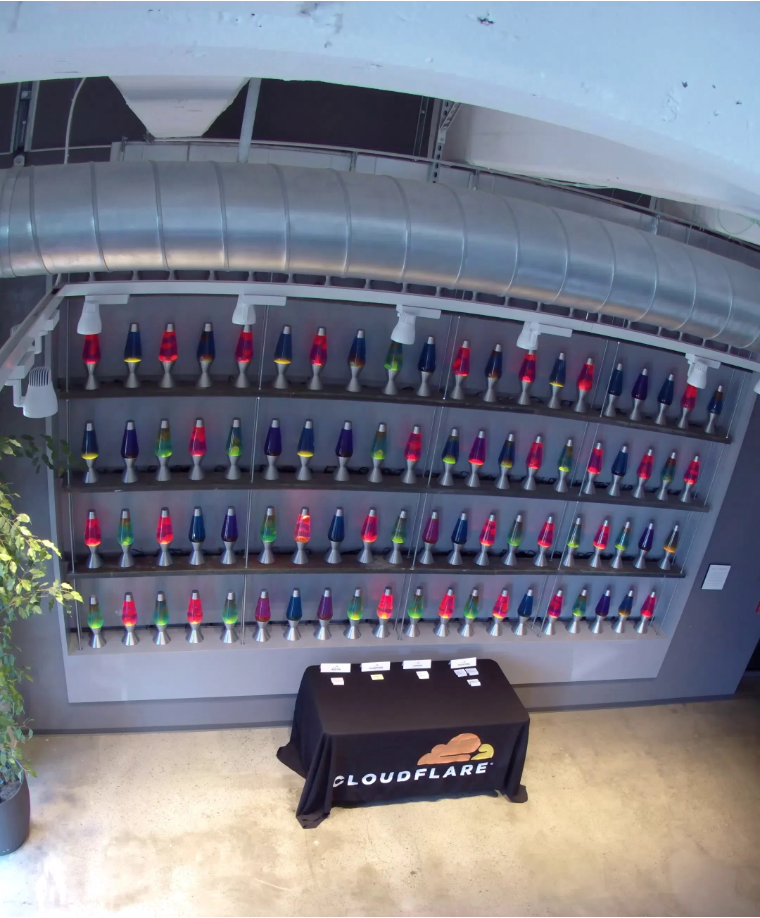
\includegraphics[width=0.4\linewidth]{chapters/02-teoria/figures/lavarandCamera}
    \caption{Widok z kamery w biurze Cloudflare~\cite{cloudflare_lavarand}.}
    \label{fig:lavarand}
\end{figure}


Firma ta oferuje użytkownikom dostęp do generatora liczb losowych w chmurze, który jest wykorzystywany
m.in. do tworzenia kluczy kryptograficznych oraz w innych zastosowaniach wymagających silnych zabezpieczeń.
Dzięki wykorzystaniu globalnej infrastruktury Cloudflare generowane liczby losowe są
szeroko dostępne i charakteryzują się dużą niezawodnością oraz odpornością na ataki.


\section{Przegląd komercyjnych rozwiązań TRNG}

Współczesne systemy kryptograficzne oraz aplikacje wymagają generowania liczb losowych, które muszą charakteryzować się wysoką jakością i odpornością na przewidywalność. Najlepiej spełniają do generatory liczb losowych oparte na fizycznych zjawiskach, zwane TRNG (True Random Number Generator). TRNG są szczególnie istotne w kontekście aplikacji wymagających silnej ochrony danych, takich jak systemy kryptograficzne, podpisy cyfrowe, oraz w generowaniu kluczy szyfrujących.

\subsection{Rozwiązania sprzętowe}

Wśród komercyjnych rozwiązań sprzętowych, wiodącymi producentami są firmy takie jak \textbf{ID Quantique}, \textbf{Microchip Technology} i \textbf{Semtech}, które oferują zaawansowane urządzenia bazujące na TRNG. Produkty te zapewniają wysoki poziom bezpieczeństwa i są stosowane w wymagających aplikacjach, takich jak bankowość elektroniczna czy systemy wojskowe.

\begin{itemize}
    \item \textbf{ID Quantique} jest jednym z liderów w dziedzinie generatorów liczb losowych opartych na technologii fotoniki. Firma oferuje urządzenia, które wykorzystują detekcję fotonów w celu generowania liczb losowych. Dzięki temu rozwiązania ID Quantique charakteryzują się bardzo wysoką jakością losowości, a jednocześnie są odporne na ataki związane z analizą i przewidywaniem generowanych liczb.

    \item \textbf{Microchip Technology} w swojej ofercie posiada różne moduły TRNG, w tym układy scalone, które generują liczby losowe na podstawie fluktuacji szumów termicznych. Produkty te znajdują zastosowanie w szerokim zakresie aplikacji, od urządzeń mobilnych po systemy wbudowane.

    \item \textbf{Semtech} natomiast oferuje rozwiązania, które wykorzystują zjawiska losowe zachodzące w obwodach analogowych do generowania liczb losowych. Firma ta jest jednym z głównych dostawców układów TRNG, które znajdują szerokie zastosowanie w urządzeniach IoT oraz w systemach komunikacji bezprzewodowej.
\end{itemize}

\subsection{Generatory TRNG w chmurze}

W ostatnich latach pojawiły się także rozwiązania chmurowe, które umożliwiają generowanie liczb losowych w czasie rzeczywistym bez potrzeby posiadania własnego sprzętu. Przykładem takiego rozwiązania jest \textbf{Cloudflare} – firma specjalizująca się w dostarczaniu usług związanych z bezpieczeństwem sieciowym. Na swoim blogu Cloudflare przedstawia zaawansowane metody generowania liczb losowych, które są wykorzystywane w ich systemach.
Cloudflare korzysta z technologii opartych na zjawiskach fizycznych, takich jak "Entropy Wall", czyli seed'owanie PRNG za pomocą danych pochodzących z kamery, ze zdjęć ściany lamp lawowych*,
nieprzewidywalnego fizycznie trójstopniowego wahadła, rozpadu radioaktywnego Uranu oraz procesów związane z tzw. "chaosem kwantowym".
Tego typu rozwiązania pozwalają na szybkie i bezpieczne generowanie liczb losowych w skali globalnej, zapewniając jednocześnie wysoki poziom ochrony przed atakami.

*LavaRand pozostaje dzisiaj jedynie dodatkowym zabezpieczeniem firmy, na wypadek gdyby ich konwencjonalne źródła entropii okazały się niewystarczające, jednak wciąż pozostaje inspirującym przykładem do szukania losowości wszędzie wokół nas.

% rescale?
\begin{figure}[H]
    \centering
    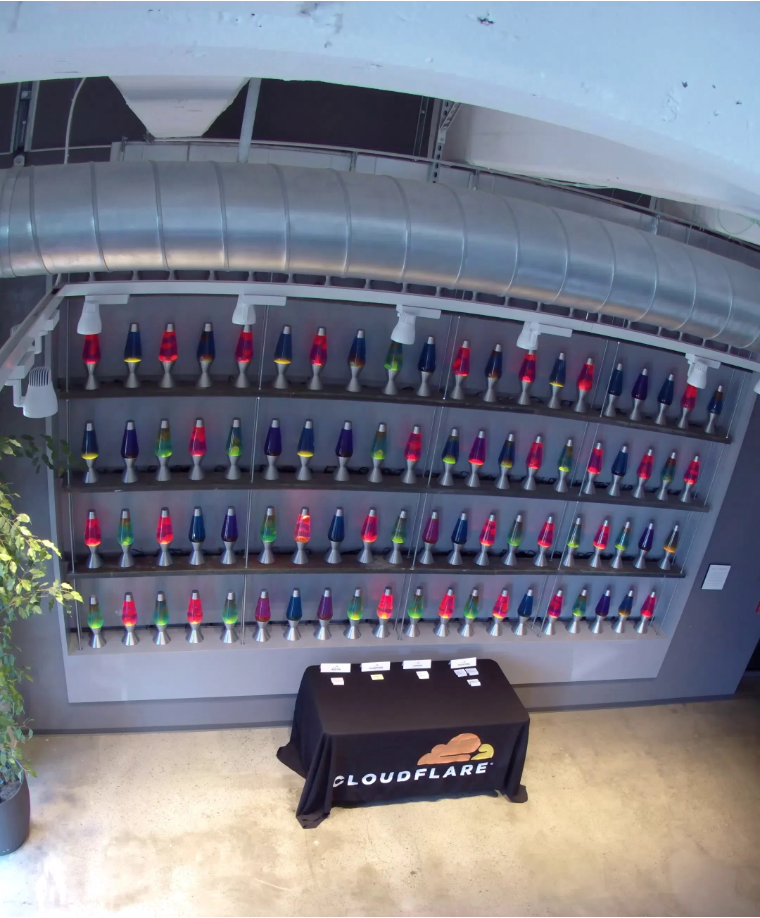
\includegraphics[width=0.4\linewidth]{chapters/02-teoria/figures/lavarandCamera}
    \caption{Widok z kamery w biurze Cloudflare}
    \label{fig:lavarand}
\end{figure}
Źródło: https://blog.cloudflare.com/lavarand-in-production-the-nitty-gritty-technical-details/
TODO - dodać do bibtex'a ;)

Firma ta oferuje użytkownikom dostęp do generatora liczb losowych w chmurze, który jest wykorzystywany
m.in. do tworzenia kluczy kryptograficznych oraz w innych zastosowaniach wymagających silnych zabezpieczeń.
Dzięki wykorzystaniu globalnej infrastruktury Cloudflare generowane liczby losowe są
szeroko dostępne i charakteryzują się dużą niezawodnością oraz odpornością na ataki.


        -----TODO---- \\
    Zrobić mniej poszatkowane \\
    idk kto to zrobi najlepiej, ale w wolnej chwili zerknijcie tu proszę \\
    I TAK ZOSTAWIAM TO W PDF, ŻEBYŚCIE PRZEGLĄDAJĄC NA TO TRAFILI! \\


\section{Wady dostępnych rozwiązań TRNG}

Mimo że Generatory Liczb Losowych Oparte na Zjawiskach Fizycznych (TRNG) oferują wysoki poziom bezpieczeństwa i losowości, istnieje kilka istotnych wad i ograniczeń związanych z ich implementacją i użytkowaniem. Wśród głównych problemów, które mogą wpływać na wydajność oraz niezawodność TRNG, wyróżnia się następujące aspekty:

\subsection{Wydajność i szybkość generowania liczb losowych}

Wydajność TRNG jest często niższa niż w przypadku Generujących Liczby Losowe Oparte na Algorytmach (PRNG). Generowanie liczb losowych za pomocą zjawisk fizycznych, takich jak szum termiczny czy fluktuacje kwantowe, może być procesem czasochłonnym, szczególnie w systemach wymagających dużych ilości losowych liczb w krótkim czasie. W wyniku tego, TRNG mogą nie spełniać wymagań wydajnościowych w aplikacjach o dużym zapotrzebowaniu na losowość, takich jak systemy kryptograficzne o bardzo wysokiej częstotliwości operacji.

\subsection{Koszty implementacji}

Urządzenia TRNG, zwłaszcza te oparte na zaawansowanych technologiach, takich jak fotonika kwantowa czy detekcja szumów kwantowych, mogą wiązać się z wysokimi kosztami produkcji oraz utrzymania. Z tego powodu, TRNG są często droższe w porównaniu do bardziej ekonomicznych rozwiązań opartych na algorytmach deterministycznych (PRNG), które wystarczają do wielu zastosowań, gdzie wysoka jakość losowości nie jest kluczowym wymaganiem.

\subsection{Stabilność i jakość generowanych liczb losowych}

Choć TRNG są uznawane za bezpieczne, ich jakość może być wpływana przez różne czynniki zewnętrzne, takie jak temperatura, zakłócenia elektromagnetyczne czy inne zmiany środowiskowe. W wyniku tego, generowane liczby losowe mogą wykazywać pewne niskiej jakości właściwości, co wymaga zastosowania dodatkowych mechanizmów, takich jak procesy post-przetwarzania, aby zapewnić ich odpowiednią losowość. Nawet małe zakłócenia w systemie mogą prowadzić do wzorców, które mogą zostać wykorzystane w atakach kryptograficznych.

\subsection{Skomplikowana kalibracja i konserwacja}

Urządzenia TRNG, szczególnie te, które wykorzystują skomplikowane zjawiska fizyczne, wymagają starannej kalibracji i ciągłego monitorowania, aby zapewnić ich prawidłowe funkcjonowanie. W wielu przypadkach konieczne jest stosowanie systemów nadzoru, które monitorują jakość generowanych liczb losowych w czasie rzeczywistym. Ponadto, wymogi dotyczące utrzymania odpowiednich warunków pracy, takich jak stabilna temperatura czy brak zakłóceń elektromagnetycznych, mogą stanowić dodatkową przeszkodę w ich szerokim zastosowaniu.

\subsection{Złożoność integracji z istniejącymi systemami}

Integracja TRNG z już działającymi systemami, zwłaszcza w kontekście urządzeń wbudowanych lub systemów o dużych wymaganiach obliczeniowych, może wiązać się z wieloma trudnościami. Często konieczne jest dostosowanie sprzętu lub oprogramowania w celu zapewnienia kompatybilności i pełnej funkcjonalności. Dodatkowo, ze względu na fizyczną naturę tych urządzeń, integracja z innymi komponentami może prowadzić do wzrostu kosztów oraz złożoności całego systemu.

\subsection{Ograniczona dostępność i skalowalność}

Choć rynek TRNG rośnie, nadal jest on stosunkowo niszowy w porównaniu do bardziej powszechnych rozwiązań opartych na PRNG. Ograniczona dostępność wyspecjalizowanych urządzeń TRNG, szczególnie tych, które oferują wysoką jakość generowanych liczb losowych, sprawia, że ich wdrożenie jest trudniejsze, zwłaszcza w przypadkach wymagających masowej produkcji. Ponadto, nie wszystkie rozwiązania są skalowalne, co może być problemem w przypadku aplikacji wymagających elastyczności i łatwego dostosowywania wydajności do rosnących potrzeb.

\subsection{Zagadnienia związane z bezpieczeństwem}

Chociaż TRNG zapewniają wyższy poziom bezpieczeństwa niż PRNG, nie są one całkowicie odporne na ataki. Ataki fizyczne, takie jak manipulacje w obrębie urządzenia lub przechwytywanie sygnałów z jego elementów, mogą prowadzić do kompromitacji jakości liczb losowych. Ponadto, w przypadku rozwiązań opartych na technologii chmurowej, takich jak te oferowane przez Cloudflare, istnieje ryzyko ataków związanych z przechwytywaniem lub manipulowaniem danymi w trakcie transmisji, co może wpływać na bezpieczeństwo generowanych liczb losowych.

\subsection{Podsumowanie wad TRNG}

Chociaż TRNG oferują niezrównaną jakość losowości w porównaniu do rozwiązań opartych na algorytmach, posiadają również szereg wad, które mogą ograniczać ich szerokie zastosowanie. Należy do nich niska wydajność, wysokie koszty implementacji, problemy ze stabilnością generowanych liczb losowych, złożoność integracji z systemami oraz ryzyko związane z bezpieczeństwem. W miarę jak technologia będzie się rozwijać, możliwe jest, że te ograniczenia zostaną przezwyciężone, jednak obecnie stanowią one istotne wyzwanie dla szerokiego przyjęcia TRNG w różnych aplikacjach.

\subsection{Podsumowanie dostępnych na rynku TRNG}
\section{Dostępne na rynku TRNG}\label{sec:dostepne-na-rynku-trng}


tu ogólnie

\subsection{Rozwiązania podobne do naszego}
    ---- TODO ---- \\

Tutaj rozpiszemy to co dopiero niedawno trafiło na issues, czyli to jak ktoś zrobił elektroniczny smart-dice,
oraz to jak ktoś zrobił to co nazwaliśm y wariantem "betoniarka" ale z 60 lat temu ;)

\chapter{Budowa sprzętowego generatora liczb losowych}\label{ch:budowa-sprzetowego-generatora}


\section{Projektowanie robota}\label{sec:projektowanie-robota}

\subsection{Prototypowanie}\label{subsec:prototypowanie}

Przy całym procesie budowy robota wykorzystano technologię FDM (ang. \textit{Fused Deposition Modeling}) druku 3D. Pomimo tego, że proces druku 3D, zwłaszcza w przypadku dużych i skomplikowanych elementów, może być czasochłonny, jest to najlepsza dostępna
technologia do realizacji tego rodzaju projektów. Druk 3D umożliwia tworzenie niestandardowych, precyzyjnie dopasowanych komponentów, które można 
szybko zmodyfikować w fazie projektowania i łatwo wydrukować ponownie w przypadku wprowadzenia zmian. Dzięki temu prototypowanie w projektach takich 
jak budowa robotów czy urządzeń mechanicznych jest znacznie bardziej elastyczne i tańsze w porównaniu do tradycyjnych metod, takich jak obróbka 
mechaniczna czy formowanie wtryskowe, które często wymagają kosztownego sprzętu i specjalistycznej wiedzy.
Drukarki 3D są także stosunkowo przystępne cenowo. Pozwalają one na wykorzystanie różnorodnych materiałów, takich jak tworzywa sztuczne, które są lekkie 
i trwałe, czy bardziej zaawansowane filamenty kompozytowe. Ta wszechstronność materiałowa umożliwia dostosowanie właściwości mechanicznych części, takich 
jak wytrzymałość, elastyczność lub odporność na wysokie temperatury, w zależności od wymagań projektu.
Co więcej, technologia druku 3D pozwala tworzyć skomplikowane kształty, których wykonanie innymi metodami mogłoby być niemożliwe lub wymagać kosztownych 
narzędzi. Możliwość drukowania prototypów bezpośrednio na miejscu skraca czas od koncepcji do gotowego produktu, co jest szczególnie cenne w dynamicznych 
projektach inżynierskich, takich jak konstrukcja robotów. To czyni druk 3D idealnym narzędziem w projektach, które wymagają wielokrotnego 
testowania i wprowadzania ulepszeń.

Głównym założeniem podczas projektowania i budowy robota było założenie modułowości. Oznacza to, że każdy element jest wymienny i łatwo dostępny.
Dzięki takiemu podejściu wymienianie elementów w przypadku awarii czy też małe modyfikacje wynikające z udoskonalania działania robota
są znacząco prostsze i przede wszystkim szybsze, niż gdyby cały robot był jednolitą bryłą.

Proces projektowania robota rozpoczęto od przeanalizowania różnych metod wykonywania rzutu kością. Rozważano tradycyjne rozwiązania takie kubki do gry w kości oraz baffle-box.
Innym podejściem byłoby skonstruowanie robota symulującego rzut kością za pomocą mechanicznego ramienia, jednak to rozwiązanie odrzucono ze względu na 
skomplikowaną mechanikę urządzenia. Opcje wykorzystania baffle-boxa również odrzucono ze względu na potrzebę transportu kości pomiędzy górą a dołem urządzenia. To wymagałoby
wykorzystania kolejnych mechanicznych części takich jak np. taśma transportowa.
Po przeanalizowaniu wszystkich pomysłów, zdecydowano się na rozwiązanie wykorzystujące kubek do gry w kości. Kolejnym etapem była decyzja w jaki sposób 
będzie wykonywany rzut kością. Uznano jednak, że takie rozwiązanie mogłoby się okazać trudne pod względem wykonania z kilku powodów. Po pierwsze, tłoki 
generujące odpowiednią siłę do podrzucenia kubka musiałyby działać bardzo precyzyjnie, aby zapewnić powtarzalność i właściwą wysokość rzutu. Jednakże 
wielokrotne uderzenia w mechanizm mogą prowadzić do jego szybkiego zużycia, co w konsekwencji mogłoby spowodować awarię.
Dodatkowo, konstrukcja takiego systemu tłokowego wymagałaby solidnego montażu i zastosowania materiałów odpornych na dynamiczne obciążenia, takie jak 
wibracje czy przeciążenia powstałe podczas pracy. Bez odpowiedniej sztywności konstrukcji, częste uderzenia i ruchy mogłyby powodować luzy w mechanizmie, 
a w efekcie całkowite uszkodzenie się robota.
Co więcej, projektowanie i wykonanie tłoków wraz z precyzyjnym układem sterowania wymagałoby znacznych nakładów czasu i kosztów. W przypadku pracy 
ciągłej, dodatkowym problemem mogłaby być konieczność regularnej konserwacji i napraw mechanizmu, aby zapewnić jego długotrwałą sprawność. Wszystko to 
czyni to rozwiązanie niepraktycznym dla tego projektu, szczególnie gdy możliwe są prostsze i bardziej niezawodne alternatywy. Po rozważeniu innych alternatyw
zdecydowano, że najlepszym rozwiązaniem będzie obrotowy kubek, wewnątrz którego kość porusza się i odbija od ścianek. Wariant ten roboczo nazwano \textit{betoniarką} od podobnej
zasady działania. W czasie przeglądu literatury w temacie rzutów kością znaleziono artykuł, w którym opisywany jest eksperyment, do którego wykorzystano właśnie taki 
mechanizm, ponieważ zapewnia rzut zbliżony do takiego wykonanego przez człowieka \cite{PK}. Obrotowy kubek został zaprojektowany w taki 
sposób, aby umożliwić łatwą kontrolę nad jego ruchem. Dzięki temu możliwe jest ustawienie częstotliwości obrotu oraz określenie, jak długo ma się obracać. Wszystkie te ustawienia 
można zmieniać za pomocą programu napisanego w języku Python. W praktyce oznacza to, że kubek jest połączony z silnikiem, który jest sterowany przez komputer 
Raspberry Pi. Dzięki temu za pomocą komend w kodzie możliwa jest zmiana, jak szybko i na jak długo kubek ma się obracać.
W celach testowych został skonstruowany prototypowy model robota.

Pierwszy prototyp robota składał się z metalowych prętów służących za stelaż oraz elementów wydrukowanych na drukarce 3D.
Tymi elementami były: kubek, ramię służące do montażu kubka, uchwyty do prętów oraz płytka mocująca do kamery. Dodatkowo
wykorzystano silnik prądu stałego z przekładnią 48:1 napędzający kubek oraz sterownik służący do zasilania i sterowania ruchem silnika~\cite{wheel,L298}.
Pierwszy prototyp po złożeniu przedstawiono na rys.~\ref{fig:pierwszy}.

Dokładne dane techniczne komponentów robota wykorzystanych w ostatecznej wersji robota znajdują się w sekcji~\ref{subsec:hardware}.

\begin{figure}[H]
    \centering
    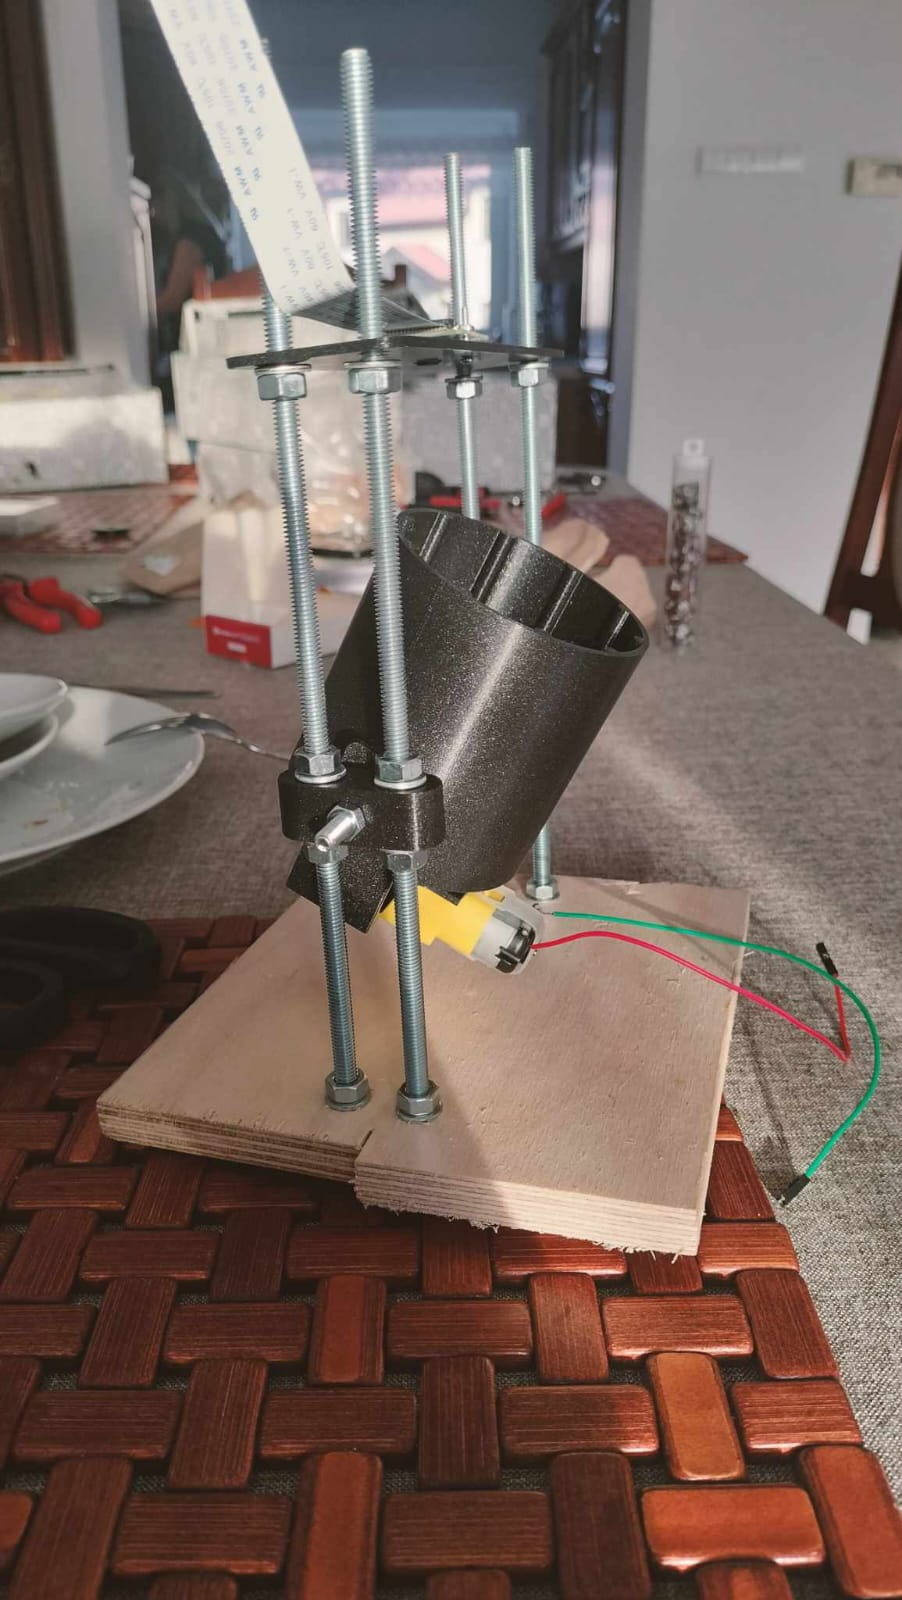
\includegraphics[width=0.25\linewidth, trim={35mm 75mm 35mm 30mm}, clip]{chapters/03-praca-wlasna/figures/pierwszy}
    \caption{\label{fig:pierwszy}Pierwszy prototyp.}
\end{figure}

Do pierwszych testów robota zaprojektowano cztery warianty kształtów kubków. Przy ich projektowaniu wymiary wzorowano na dostępnych tradycyjnych kubkach do gry w kości.
Średnice kubków do gry z reguły są w przedziale 70-90mm \cite{cup}. Przyjęto, że odpowiedni do tego zadania kubek powinien
zawierać pewnego rodzaju nierówności na ściankach. Takie samo założenie przyjęto przy wcześniej wspominanym eksperymencie \cite{PK}. Dzięki temu kość nie będzie się ślizgać po ściance a zacznie się odbijać od tych nierówności, co 
będzie lepiej imitowało rzut kością wykonany przez człowieka. Z tego powodu z założenia odrzucono tradycyjny model kubka do gry w cylindrycznym kształcie 
o gładkich ściankach. Zaprojektowano cztery wersje kubka (patrz rys.~\ref{fig:kubki}): kubek kwadratowy (nr 4), kubek sześcienny (nr 2), kubek sześcienny z dodatkowymi żebrami (nr 1)
oraz kubek cylindryczny z dodatkowymi żebrami (nr 3). 
Następnie je przetestowano umieszczając w środku kość do gry i obracając kubek wokół osi przechodzącej przez środek kubka. W czasie testów najgorzej sprawdziły się kubki sześcienne,
ponieważ kości ośmiościenne, które wykorzystywano do testów utykały w narożnikach dociskane przez siłę odśrodkową. Podobny problem pojawiał się przy testach kubka kwadratowego.
Najlepszym wariantem okazał się być cylindryczny kubek z dodatkowymi pionowymi żebrami (nr 3 na rys.~\ref{fig:kubki}), o które kość się odbijała podczas kręcenia.
Jego zaletą jest to, że nie posiada on narożników, w których kość mogłaby utknąć. Dodatkowym atutem jest niewielka masa w porównaniu z reszta testowanych wariantów co ma duże znaczenie 
przy obracaniu całego kubka ze względu na moment bezwładności \cite{bezwladnosc}.

\begin{figure}[H]
    \centering
    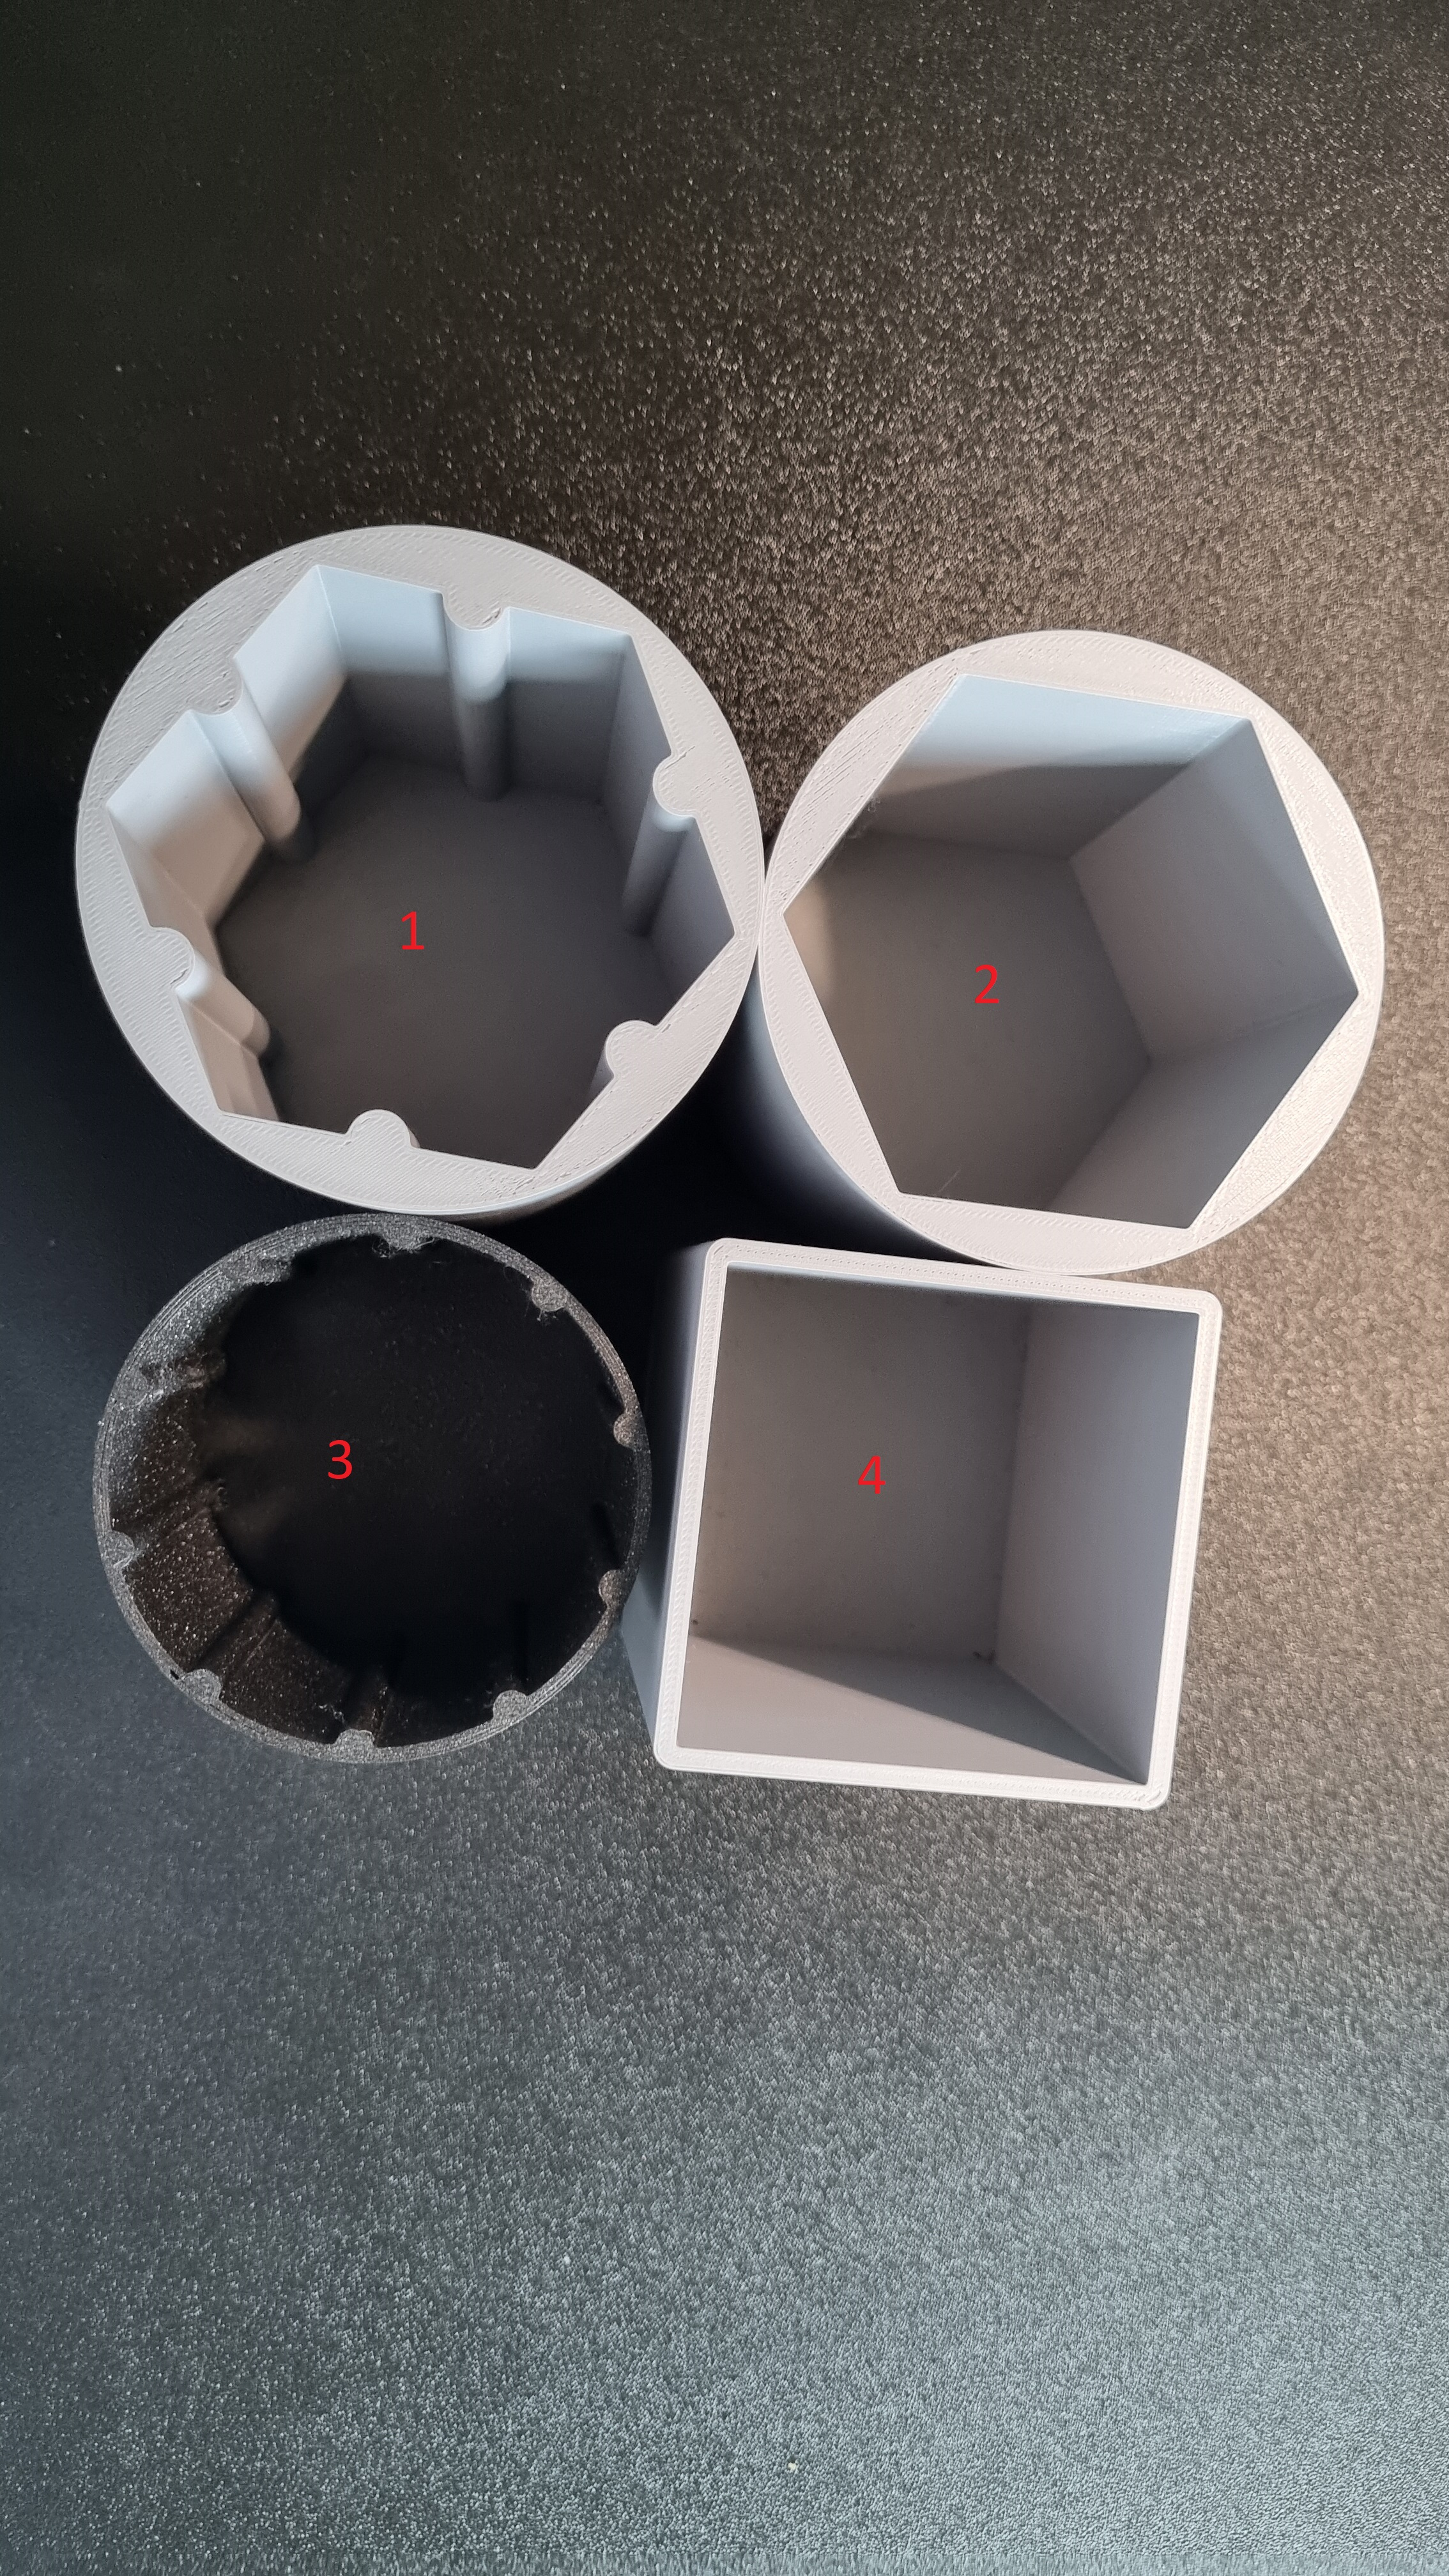
\includegraphics[width=0.65\linewidth, trim={35mm 380mm 20mm 240mm}, clip]{chapters/03-praca-wlasna/figures/kubki}
    \caption{\label{fig:kubki}Testowane warianty kubków.}
\end{figure}

Po pierwszych testach okazało się, że niezbędny do uzyskania zamierzonego efektu będzie mechanizm, który będzie 
wychylał cały kubek wraz z silnikiem, który odpowiada za jego obrót. Z początku planowano wykorzystanie
serwomechanizmu, jednak to rozwiązanie odrzucono, ponieważ większość dostępnych serwomechanizmów ma
ograniczony obrót do $180^{\circ}$ lub $360^{\circ}$, a to limitowałoby możliw ości mechanizmu służącego do wychylania kubka.
Ostatecznie w tym celu wybrano mały silnik krokowy 28BYJ-48, którego moment obrotowy 34,3mNm jest w pełni wystarczający do wychylenia kubka. 
Silnik ten obraca układem dwóch kół zębatych przedstawionych na rys.~\ref{fig:zebatki}.

\begin{figure}[H]
    \centering
    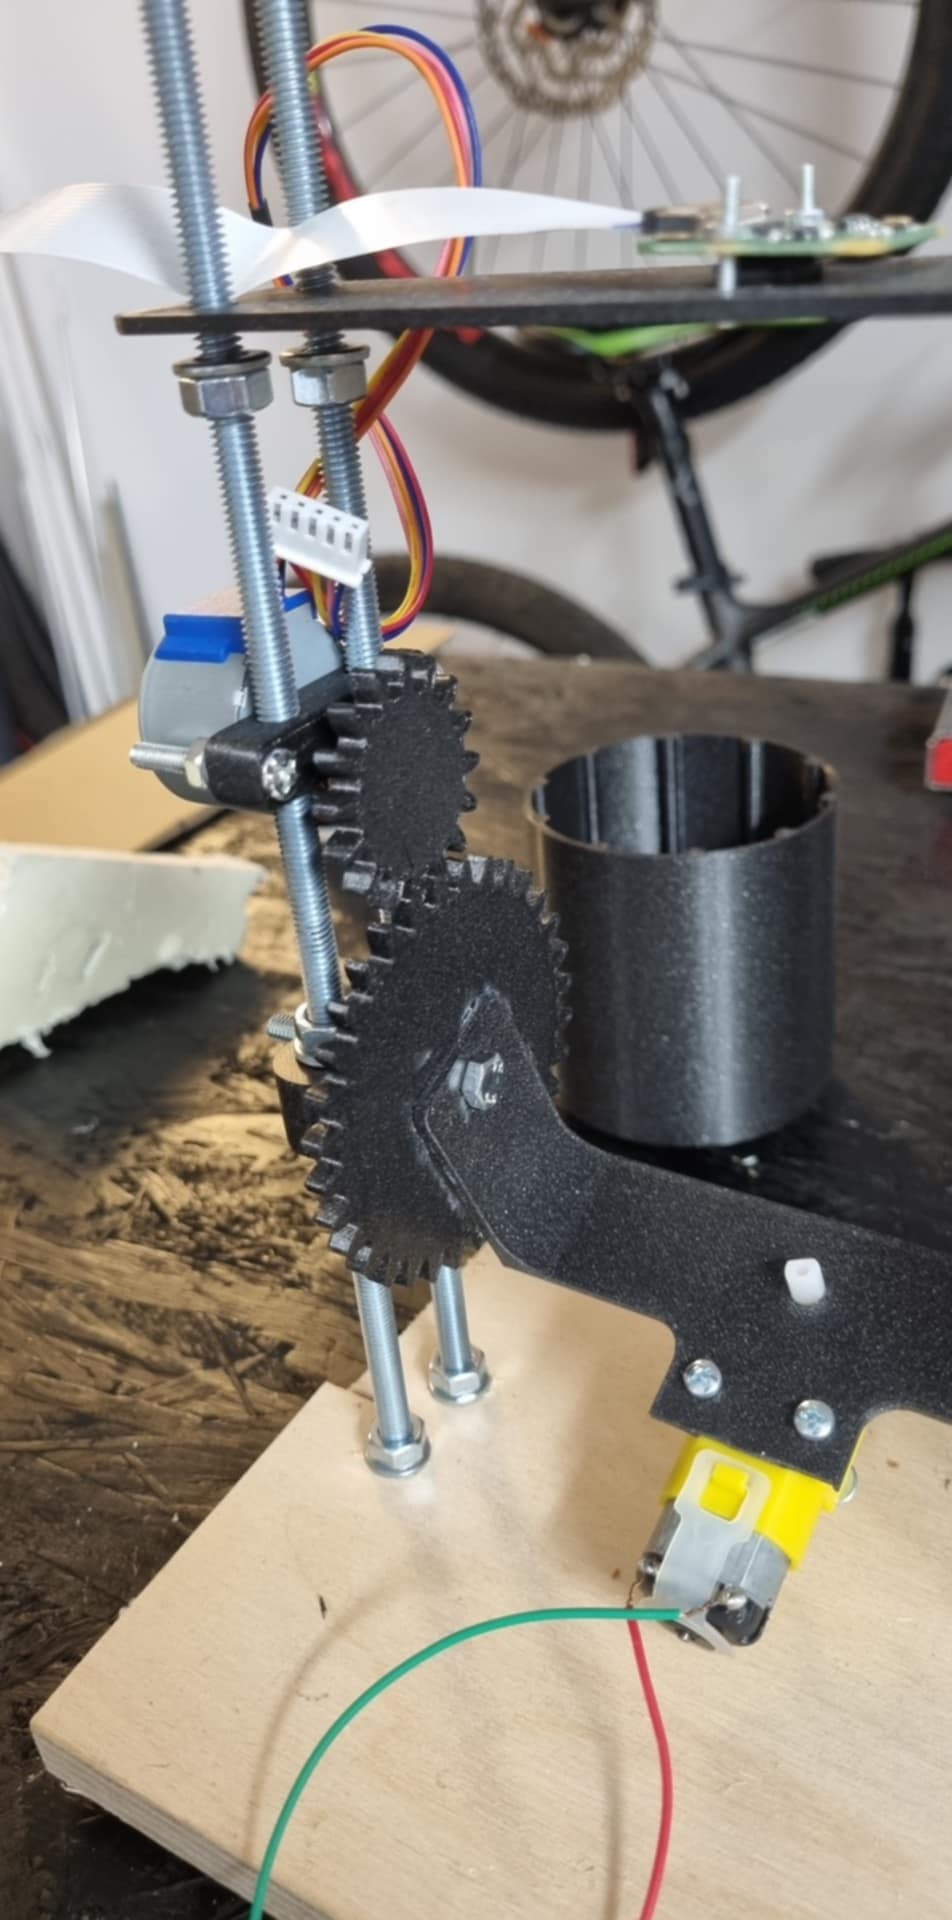
\includegraphics[width=0.25\linewidth, trim={65mm 75mm 0mm 180mm}, clip]{chapters/03-praca-wlasna/figures/koła_zębowe}
    \caption{\label{fig:zebatki}Koła zębate.}
\end{figure}

Podczas testów pierwszej wersji robota wykorzystującej obrotowy kubek powstał pomysł alternatywnego rozwiązania.
Rozwiązanie to implementuje inne podejście do rzutu kością. Zamiast obracać cały kubek, a dodatkowo wychylać go,
wykorzystany został trwale zamontowany kubek, na którego dnie znajduje się śmigło, które podcina leżącą na dnie kość.
Takie rozwiązanie znacząco upraszcza cały mechanizm robota oraz bardzo przyspiesza proces losowania liczby. Ten wariant 
nazwano roboczo \textit{blenderem} -- podobnie jak wariant \textit{betoniarki} -- od podobnej zasady działania mechanizmu.

Przy projektowaniu drugiego wariantu robota został wykorzystany ten sam stelaż złożony z metalowych prętów co w 
pierwszym wariancie. Na drukarce 3D wydrukowano dodatkowe części, niezbędne do realizacji tego wariantu.
Zaprojektowano i wydrukowano nowy kubek, śmigło oraz mocowanie dla silnika. Kubek został przystosowany do montażu 
silnika prądu stałego oraz śmigła.

W trakcie testów zauważono, że procesor robota nagrzewa się do wysokich temperatur podczas intensywnej pracy, 
co mogło negatywnie wpływać na jego wydajność i żywotność. Aby temu zapobiec, w projekcie zdecydowano się na 
zastosowanie radiatorów (rys.~\ref{fig:zimno}), które miały pomóc w rozproszeniu nadmiaru ciepła, oraz wentylatora, który 
wspomagał cyrkulację powietrza wokół procesora. Jest to działanie zalecane w oficjalnej dokumentacji na stronie Raspberry Pi, mające przeciwdziałać 
ograniczaniu wydajności w celu ochrony przed przegrzaniem (ang. \textit{Thermal throttling}) \cite{cooling}. 
Dodatkowym problemem wynikającym z rozgrzewania się procesora do wysokich temperatur jest materiał PLA, z którego wykonywane były komponenty robota
oraz prototypów. Materiał ten zaczyna się deformować przy temperature $60^{\circ}$C \cite{plaprusa}. Dzięki wykorzystaniu radiatorów oraz wentylatora udało się obniżyć temperaturę pracy
procesora, która teraz utrzymuje się w granicach $55^{\circ}$C w czasie rzutów i spada po ich zakończeniu do około $45^{\circ}$C,
co zapewnia stabilne i bezpieczne działanie całego systemu. 
\textcolor{red}{TODO sprawdzic te wartości porównac z włączonym i wyłączonym wentylatorem + dodatkowo sterowanie wentylatorem}

\begin{figure}[H]
    \centering
    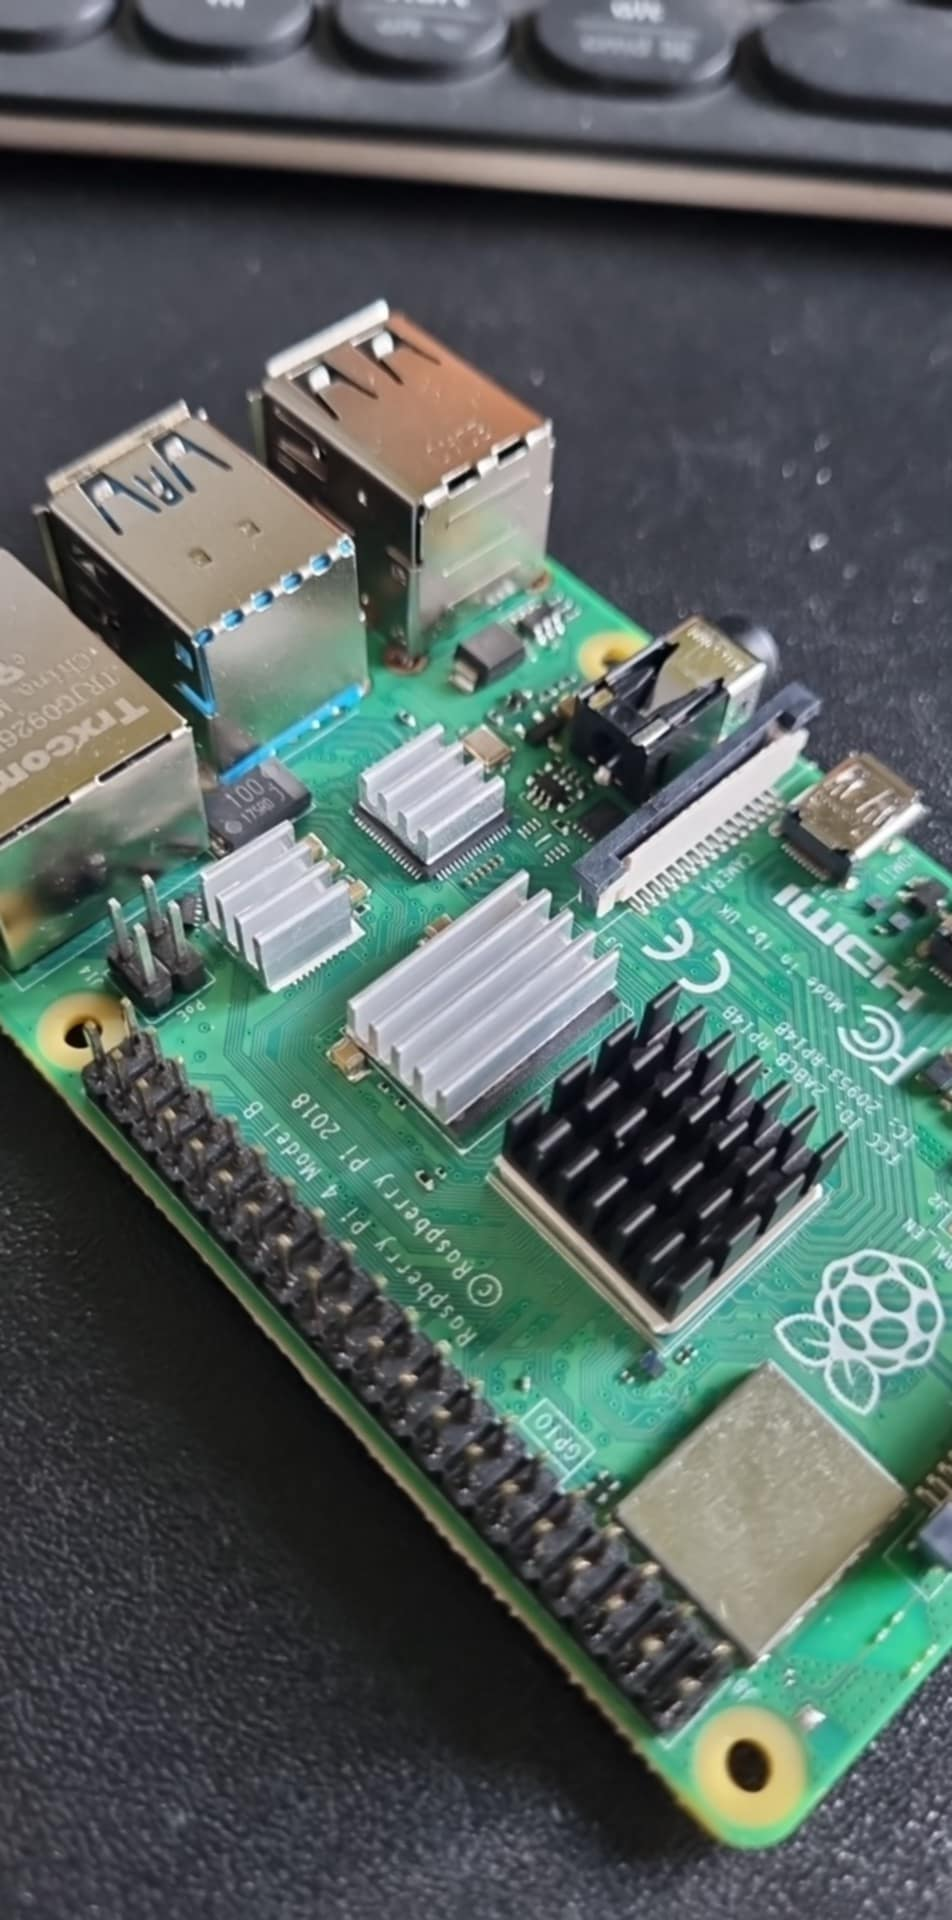
\includegraphics[width=0.25\linewidth, trim={0mm 50mm 0mm 120mm}, clip]{chapters/03-praca-wlasna/figures/now_we_are_cool}
    \caption{\label{fig:zimno}Dodane radiatory.}
\end{figure}

Duże znaczenie ma również wykorzystywana kość. Od jej koloru i tekstury zależy jakość zdjęć zrobionych przez
zamontowaną kamerę. Na Rys.~\ref{fig:zielona} - Rys.~\ref{fig:blue} przedstawiono przykładowe zdjęcia kości w różnych warianach kolorystycznych.
Na podstawie tych zdjęć wybrano kość niebieską, ponieważ numer oznaczający wynik rzutu, najlepiej kontrastuje ze ścianami kości przez co jest on najlepiej widoczny
właśnie na tej kości.

\begin{figure}[H]
    \centering
    % Pierwsze zdjęcie
    \begin{minipage}{0.32\textwidth}
        \centering
        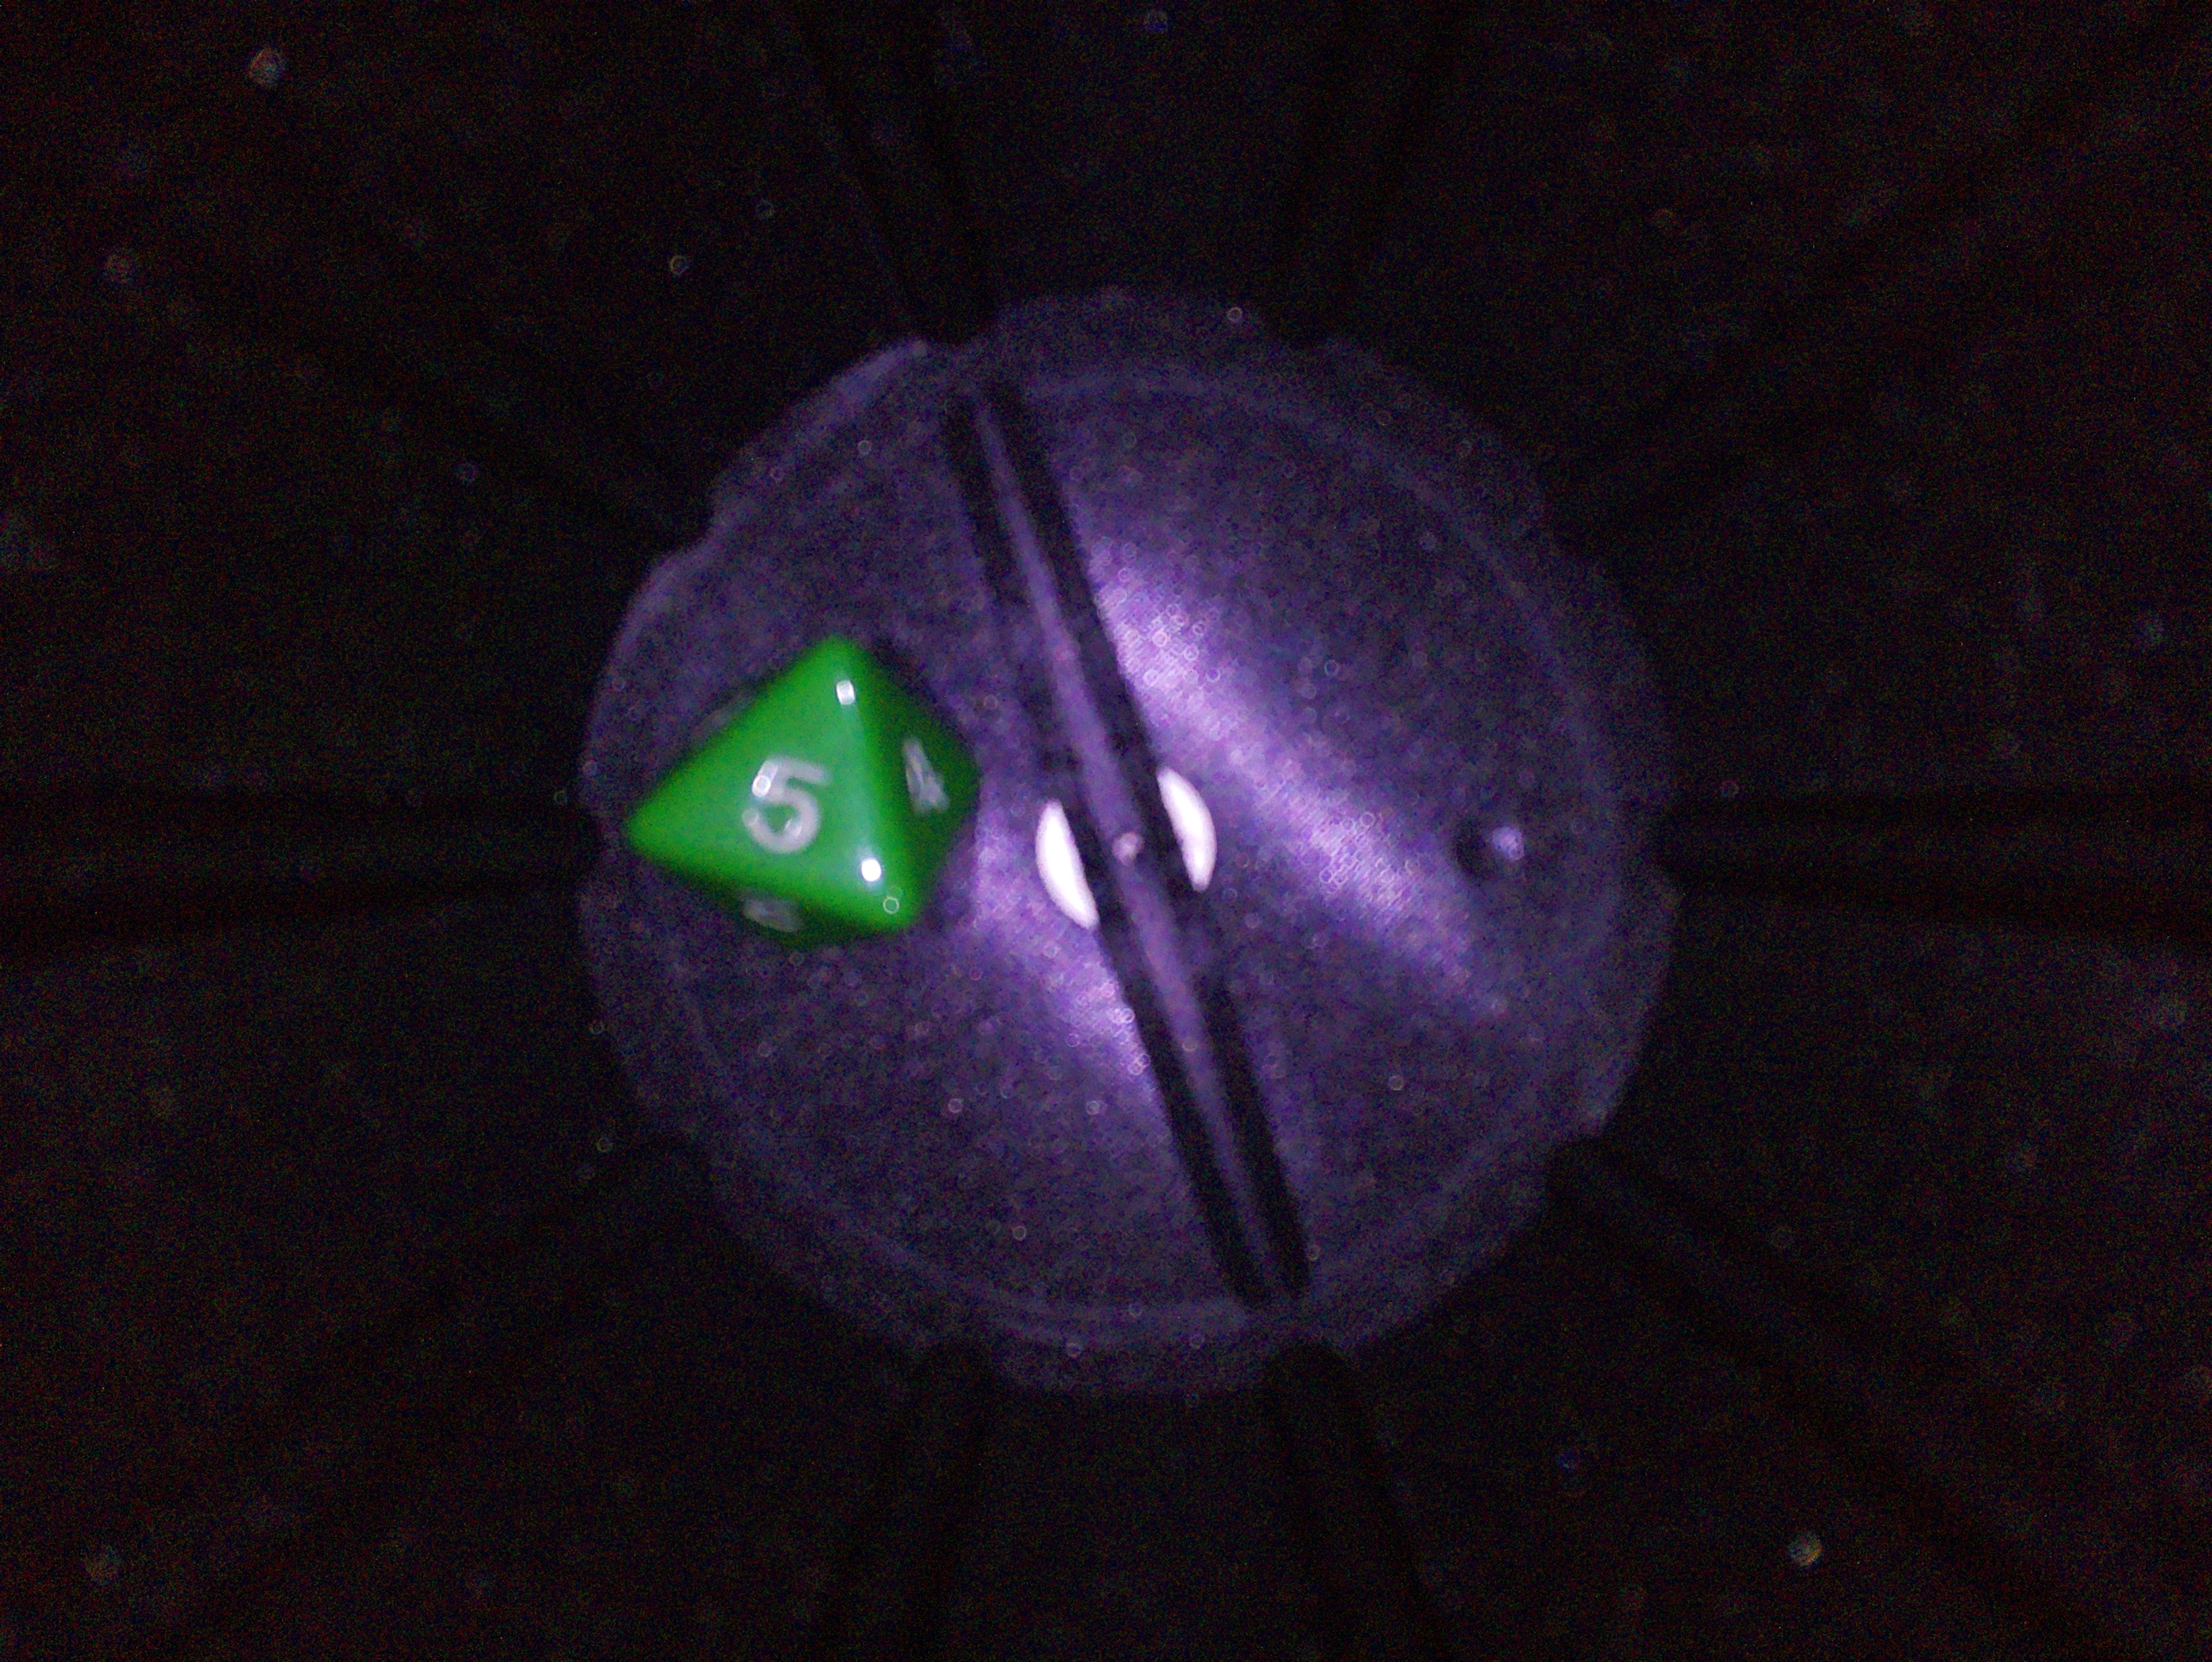
\includegraphics[width=\linewidth]{chapters/03-praca-wlasna/figures/kolorki/zielona.jpg}
        \caption{\label{fig:zielona}Pierwsze ustawienie.}
    \end{minipage}
    \hfill
    % Drugie zdjęcie
    \begin{minipage}{0.32\textwidth}
        \centering
        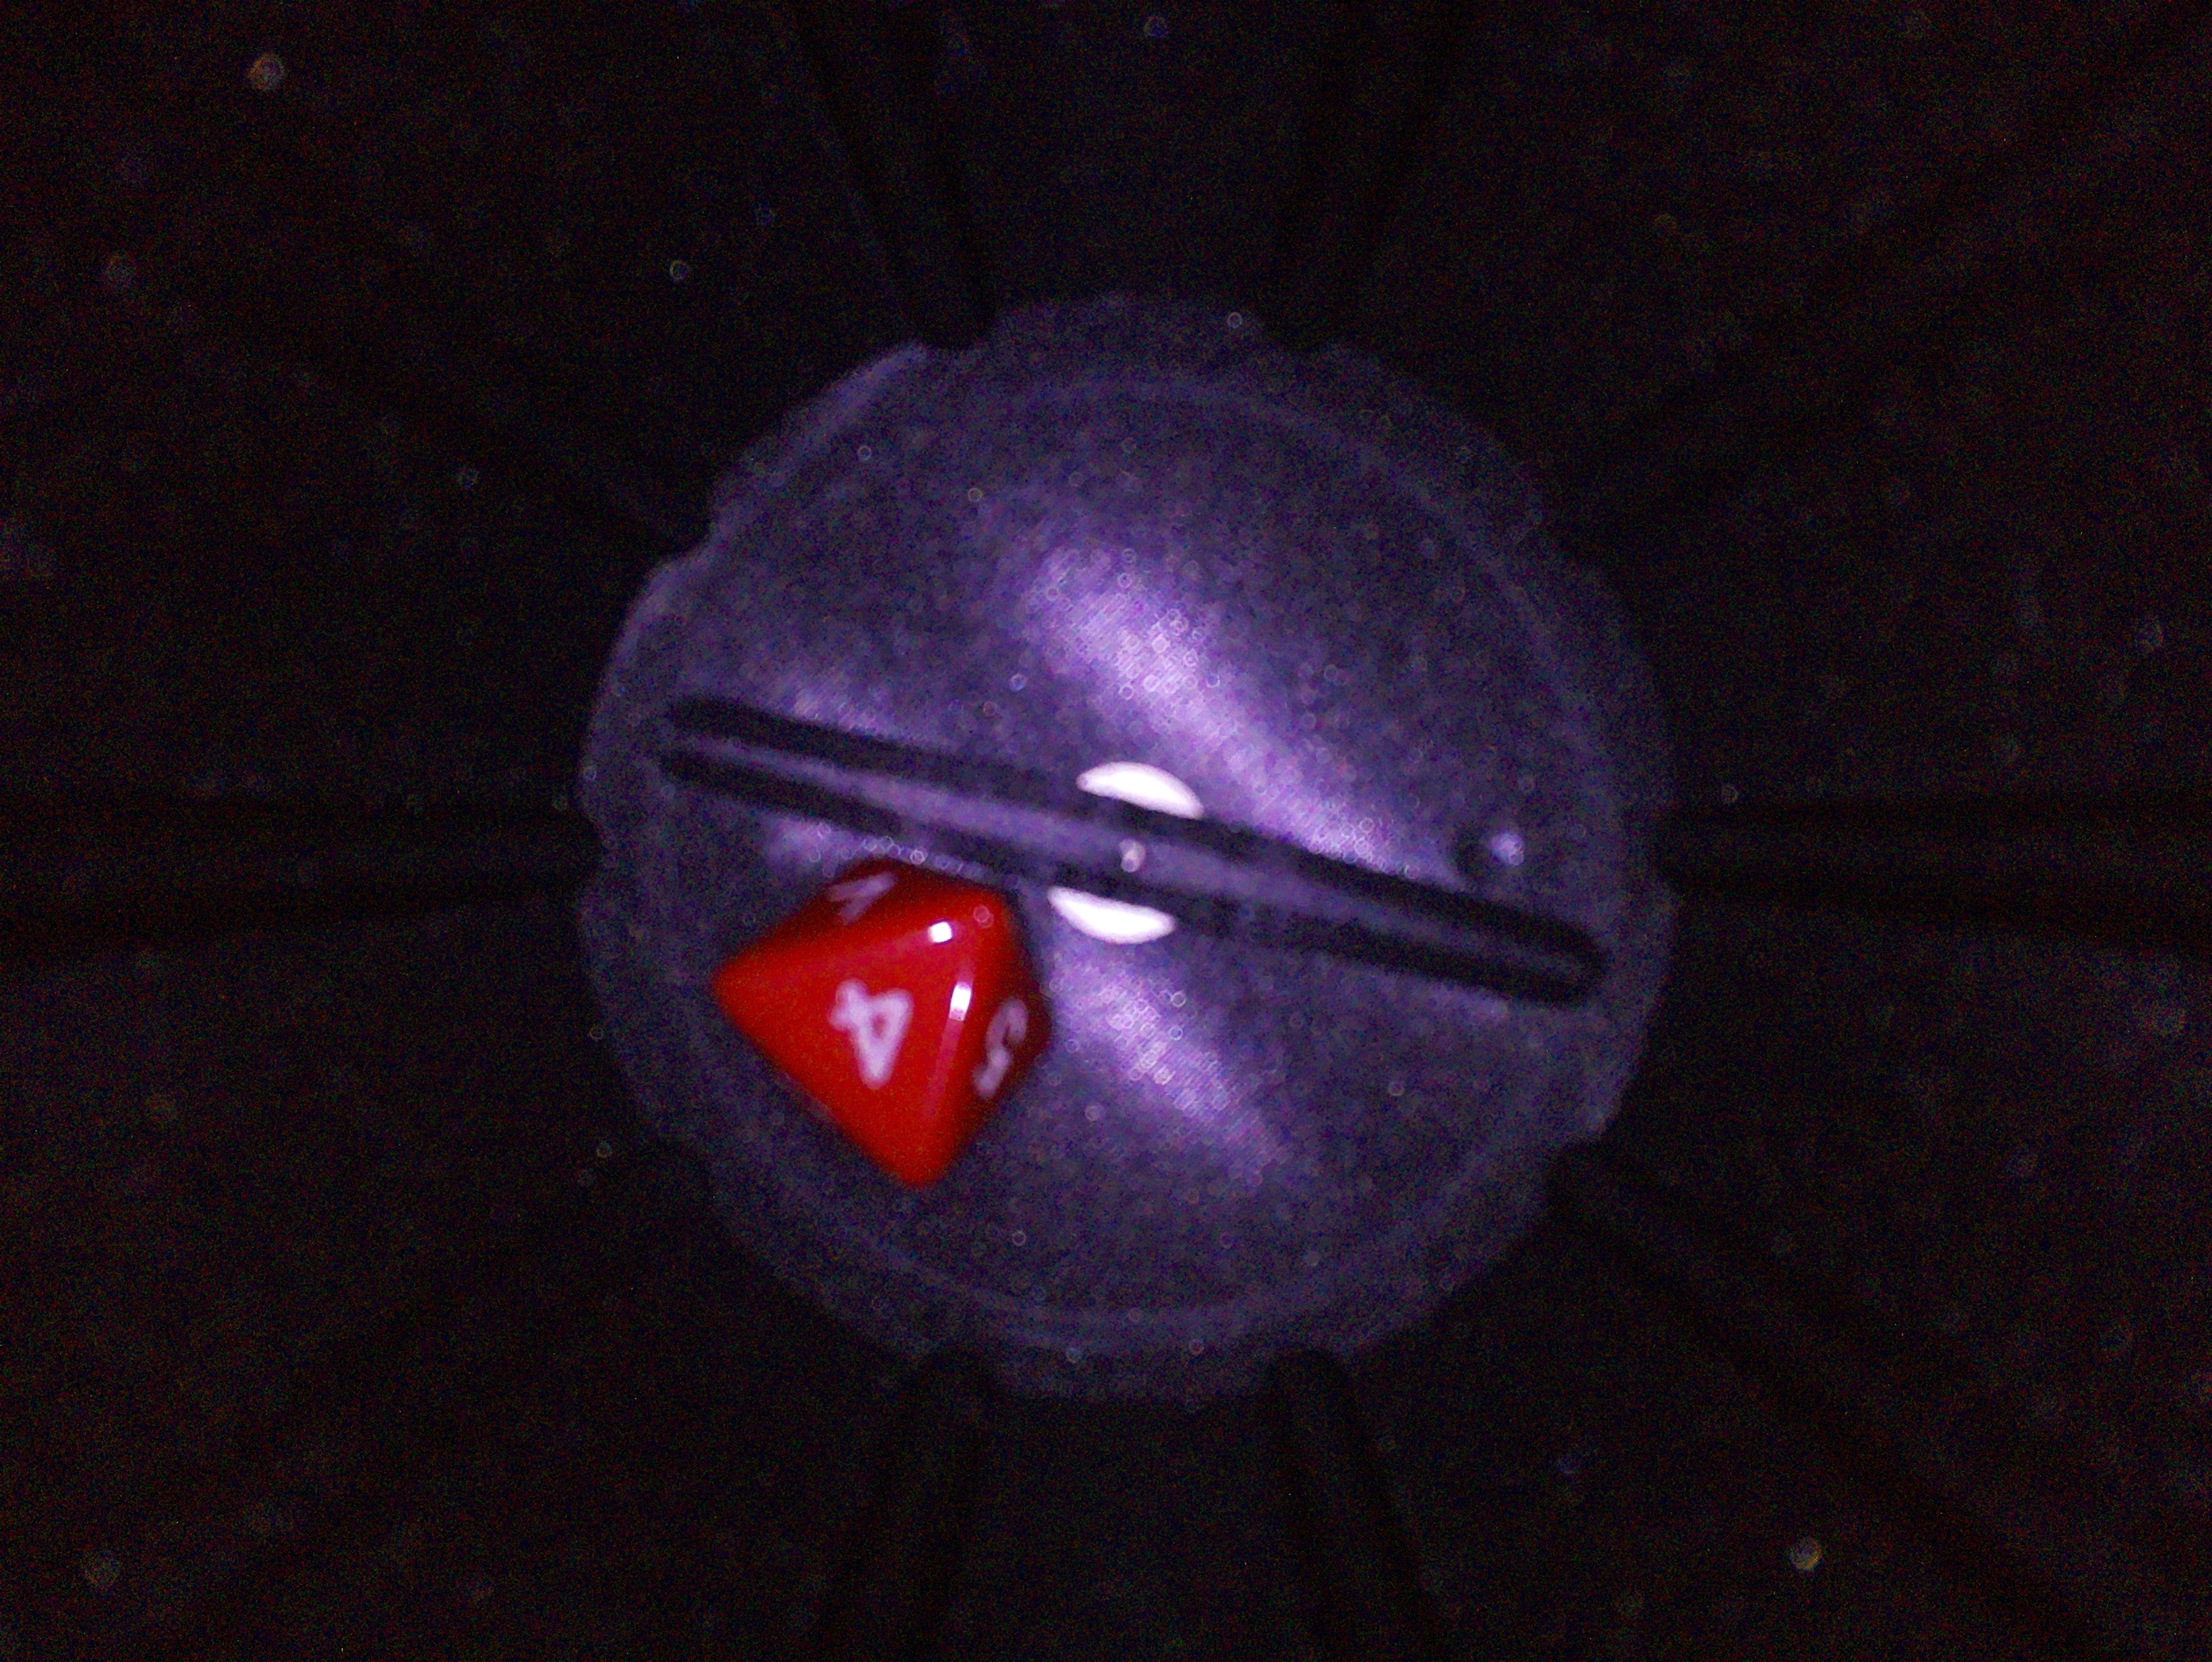
\includegraphics[width=\linewidth]{chapters/03-praca-wlasna/figures/kolorki/czerwona.jpg}
        \caption{\label{fig:czerwona}Drugie ustawienie.}
    \end{minipage}
    \hfill
    % Trzecie zdjęcie
    \begin{minipage}{0.32\textwidth}
        \centering
        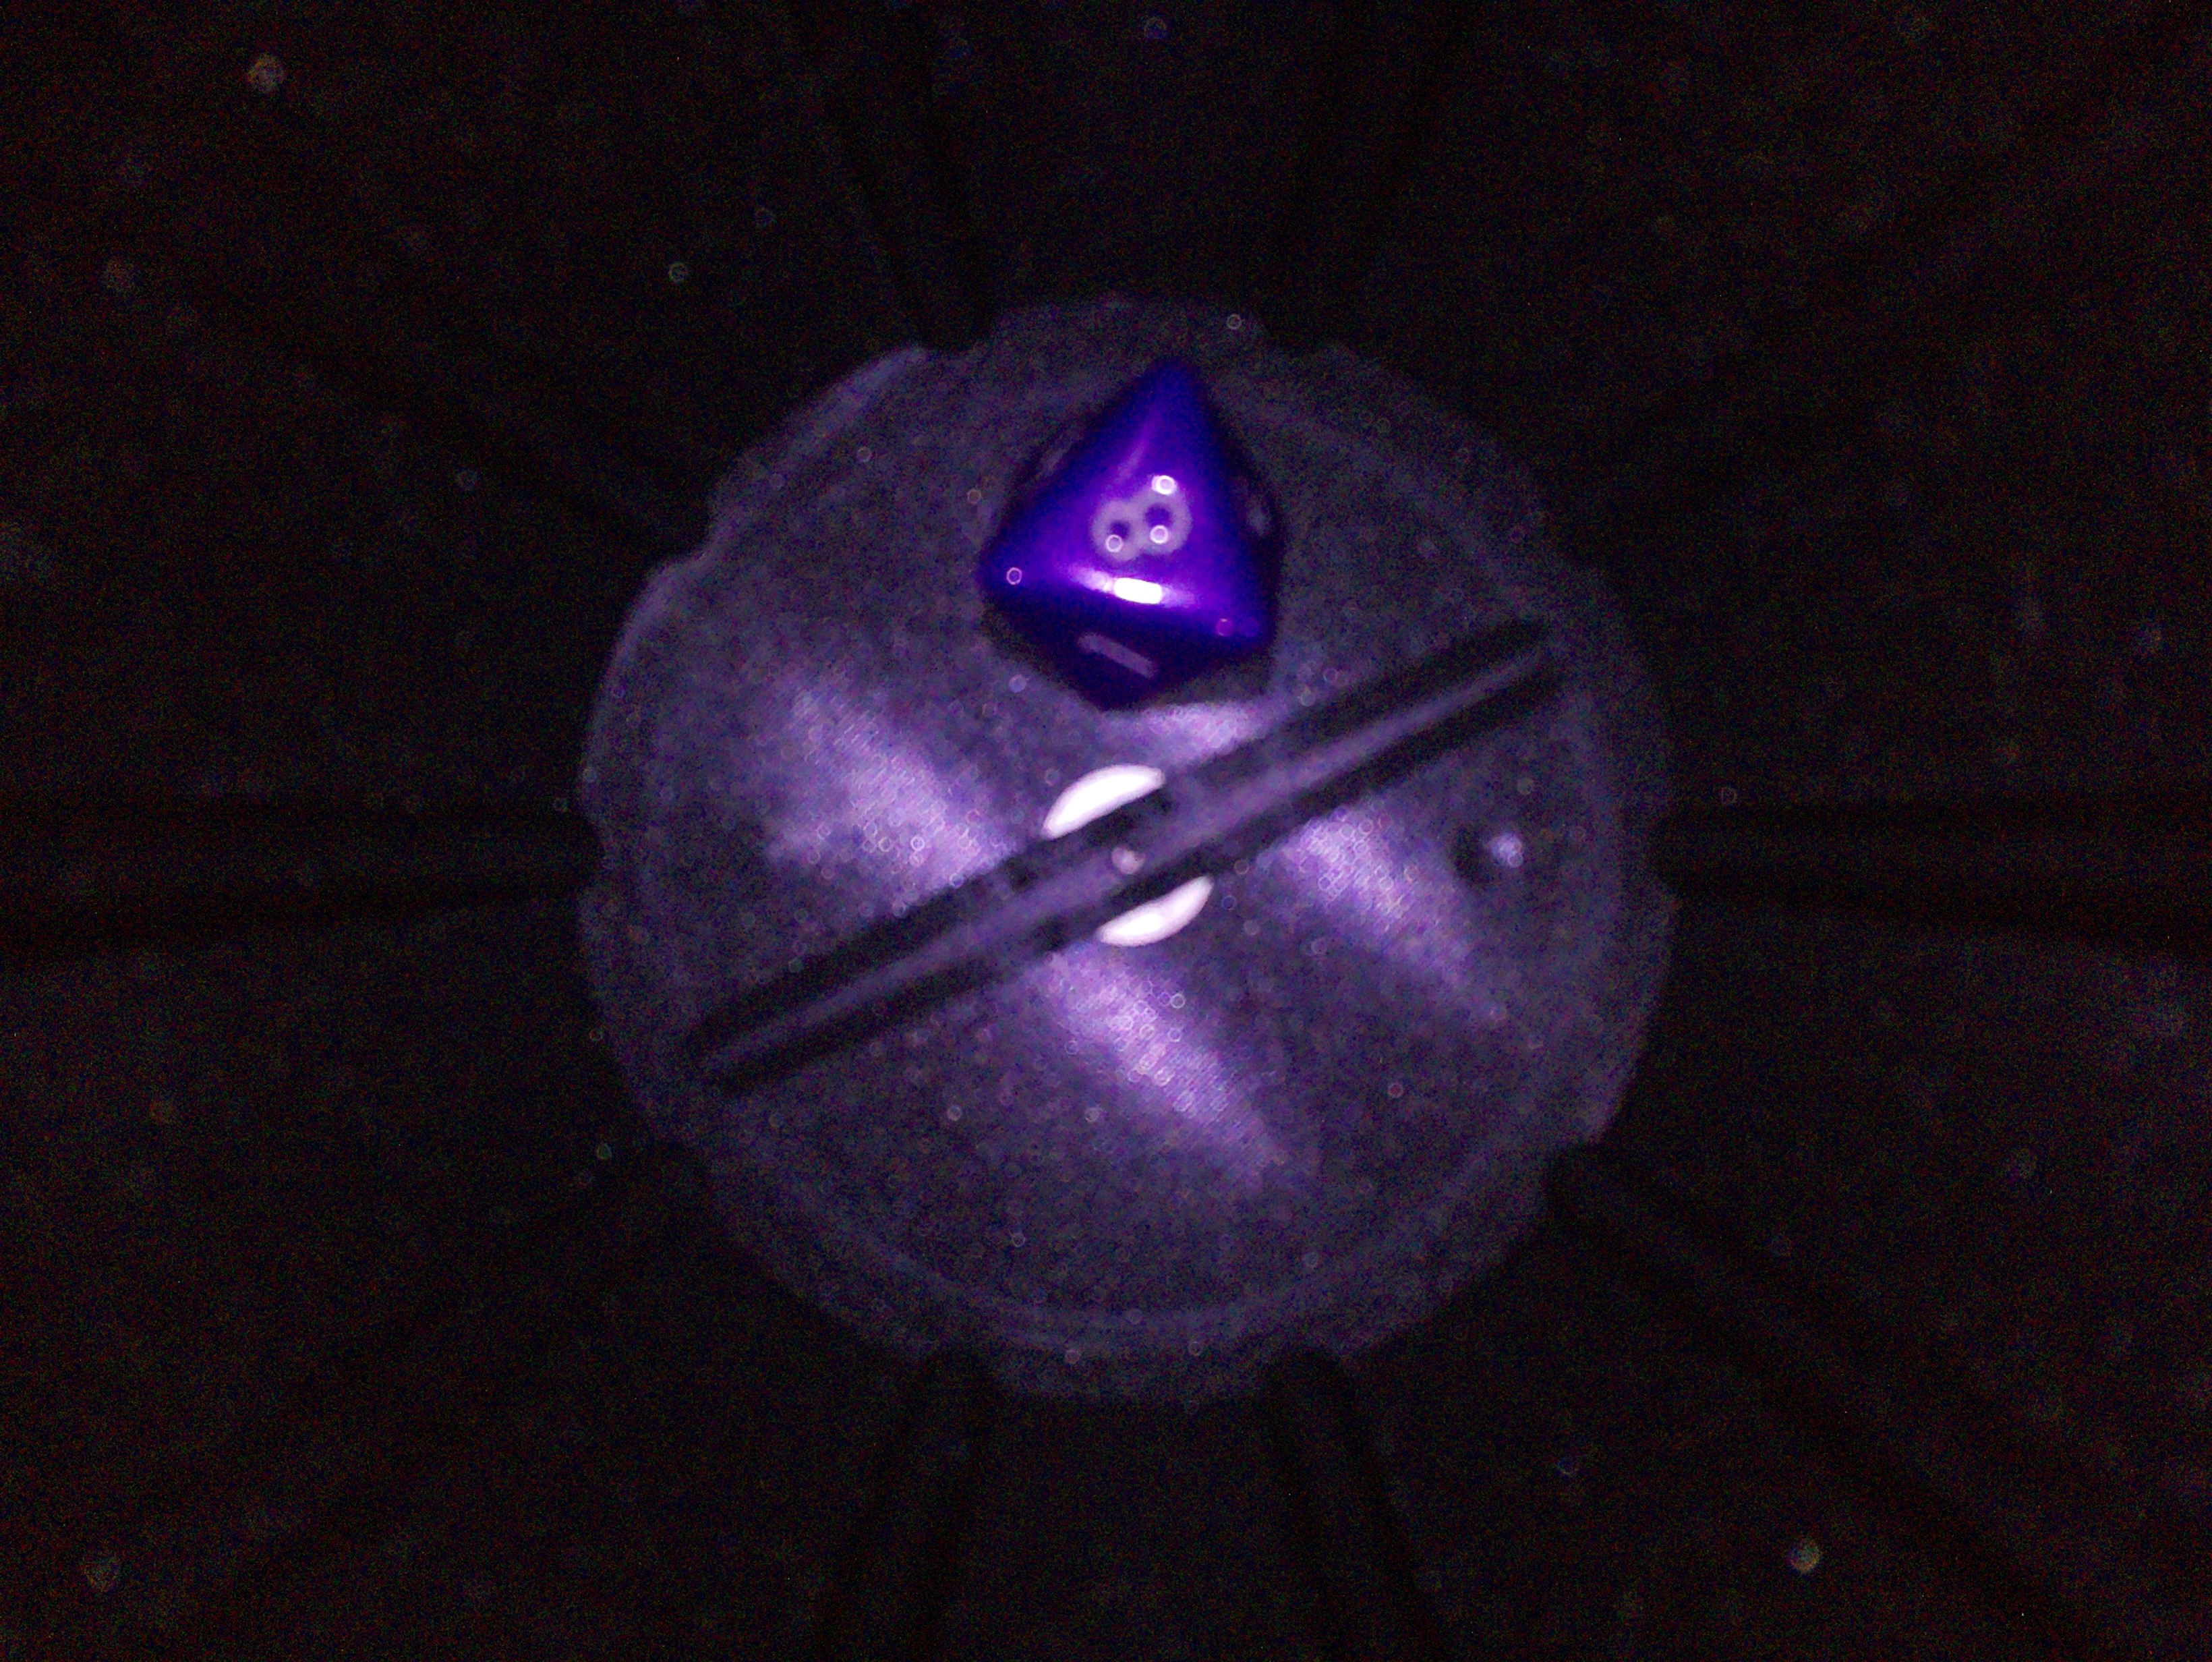
\includegraphics[width=\linewidth]{chapters/03-praca-wlasna/figures/kolorki/fiolet.jpg}
        \caption{\label{fig:fiolet}Trzecie ustawienie.}
    \end{minipage}
    \hfill
    \begin{minipage}{0.32\textwidth}
        \centering
        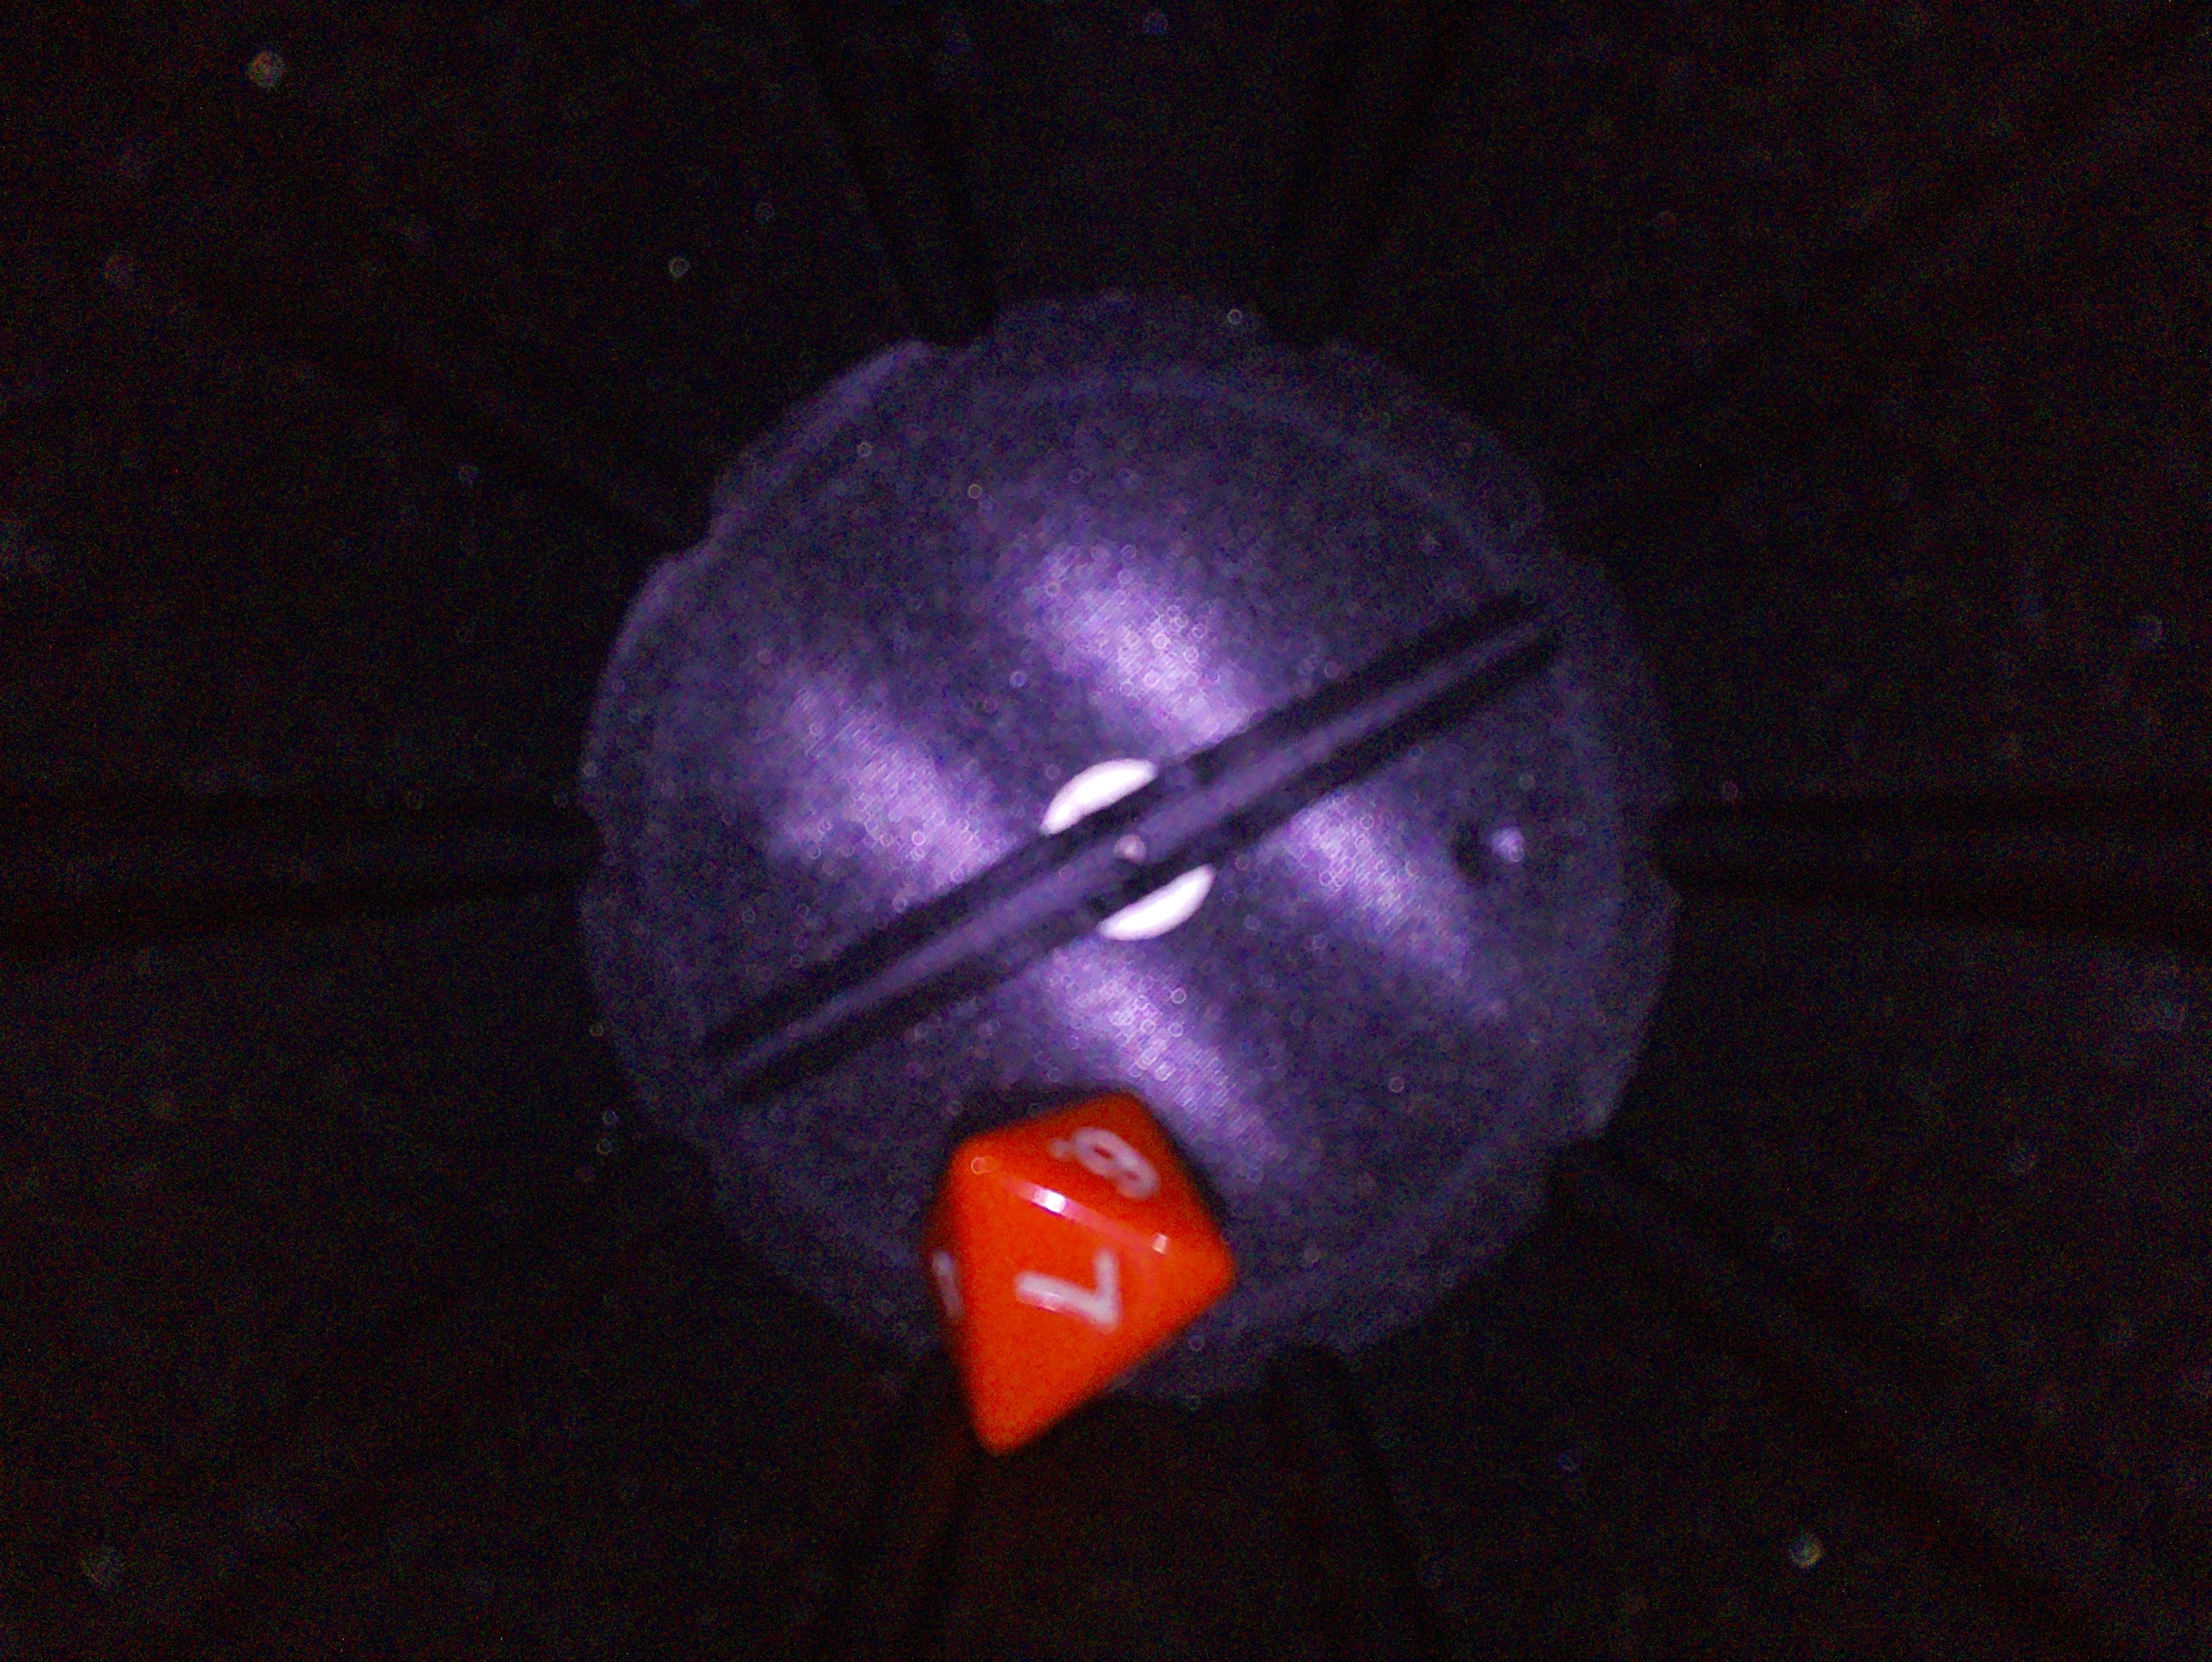
\includegraphics[width=\linewidth]{chapters/03-praca-wlasna/figures/kolorki/pomaranczowa.jpg}
        \caption{\label{fig:orange}Trzecie ustawienie.}
    \end{minipage}
    \hfill
    \begin{minipage}{0.32\textwidth}
        \centering
        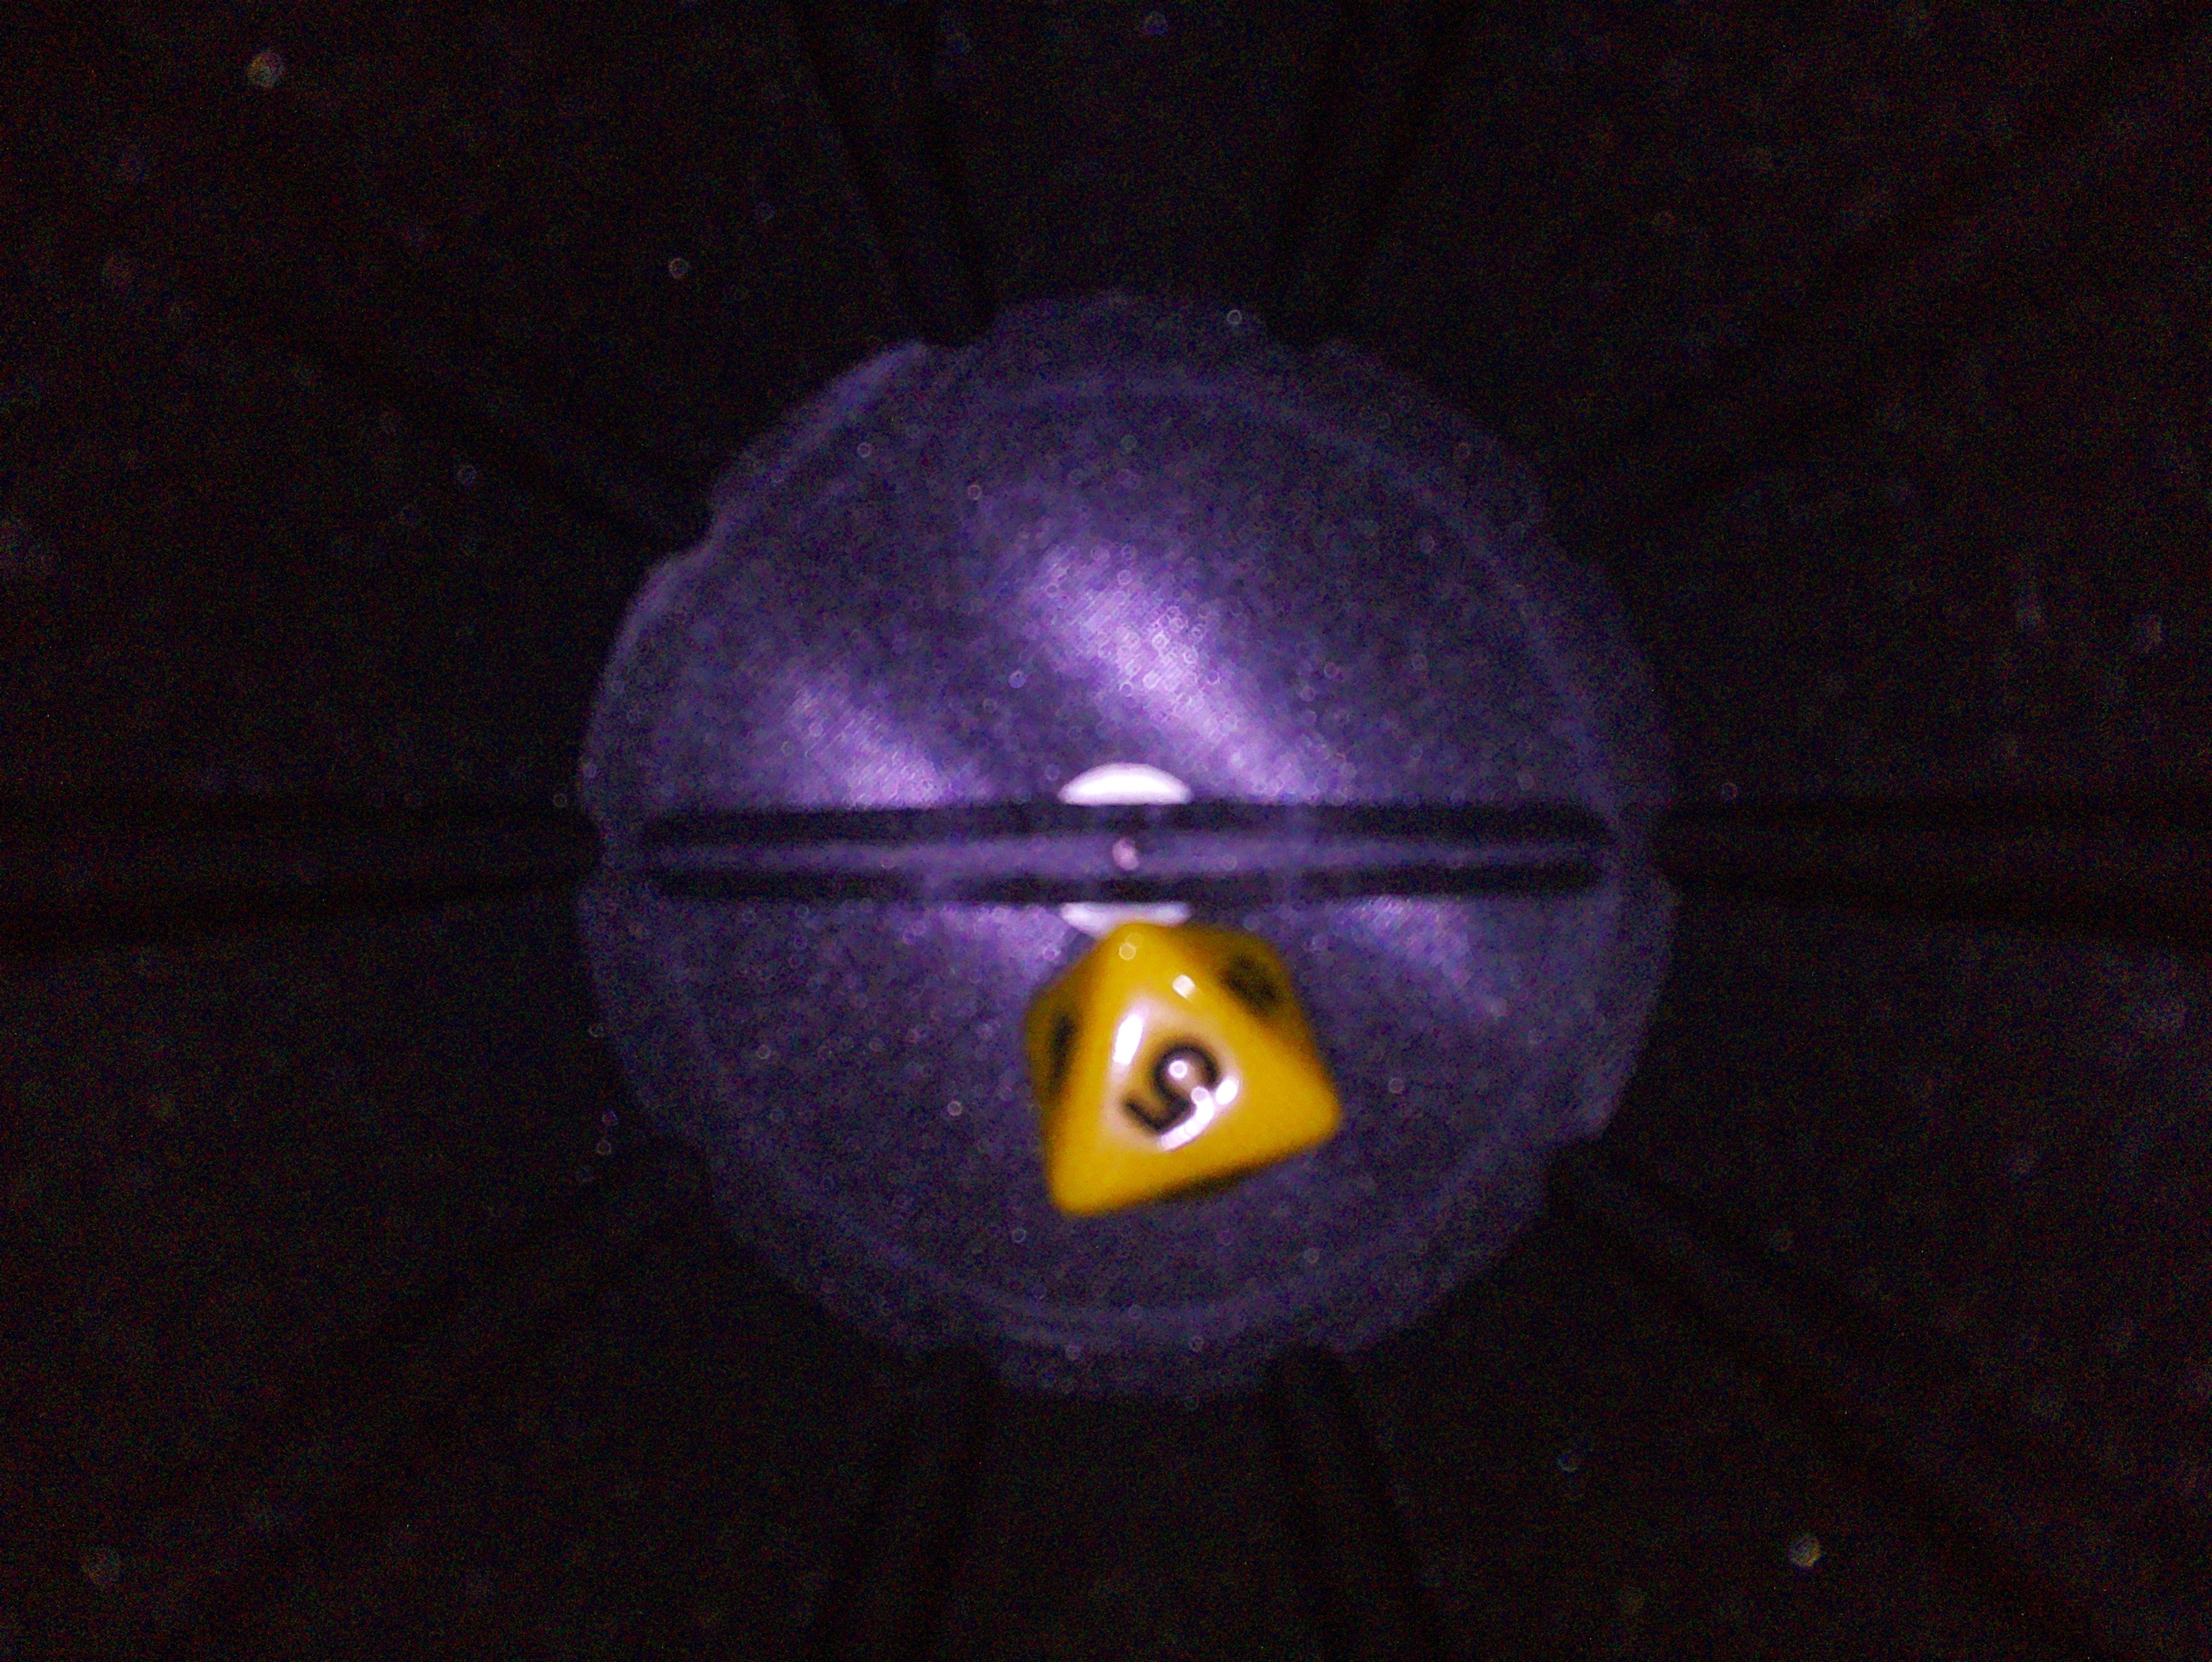
\includegraphics[width=\linewidth]{chapters/03-praca-wlasna/figures/kolorki/zolte.jpg}
        \caption{\label{fig:yellow}Trzecie ustawienie.}
    \end{minipage}
    \hfill
    \begin{minipage}{0.32\textwidth}
        \centering
        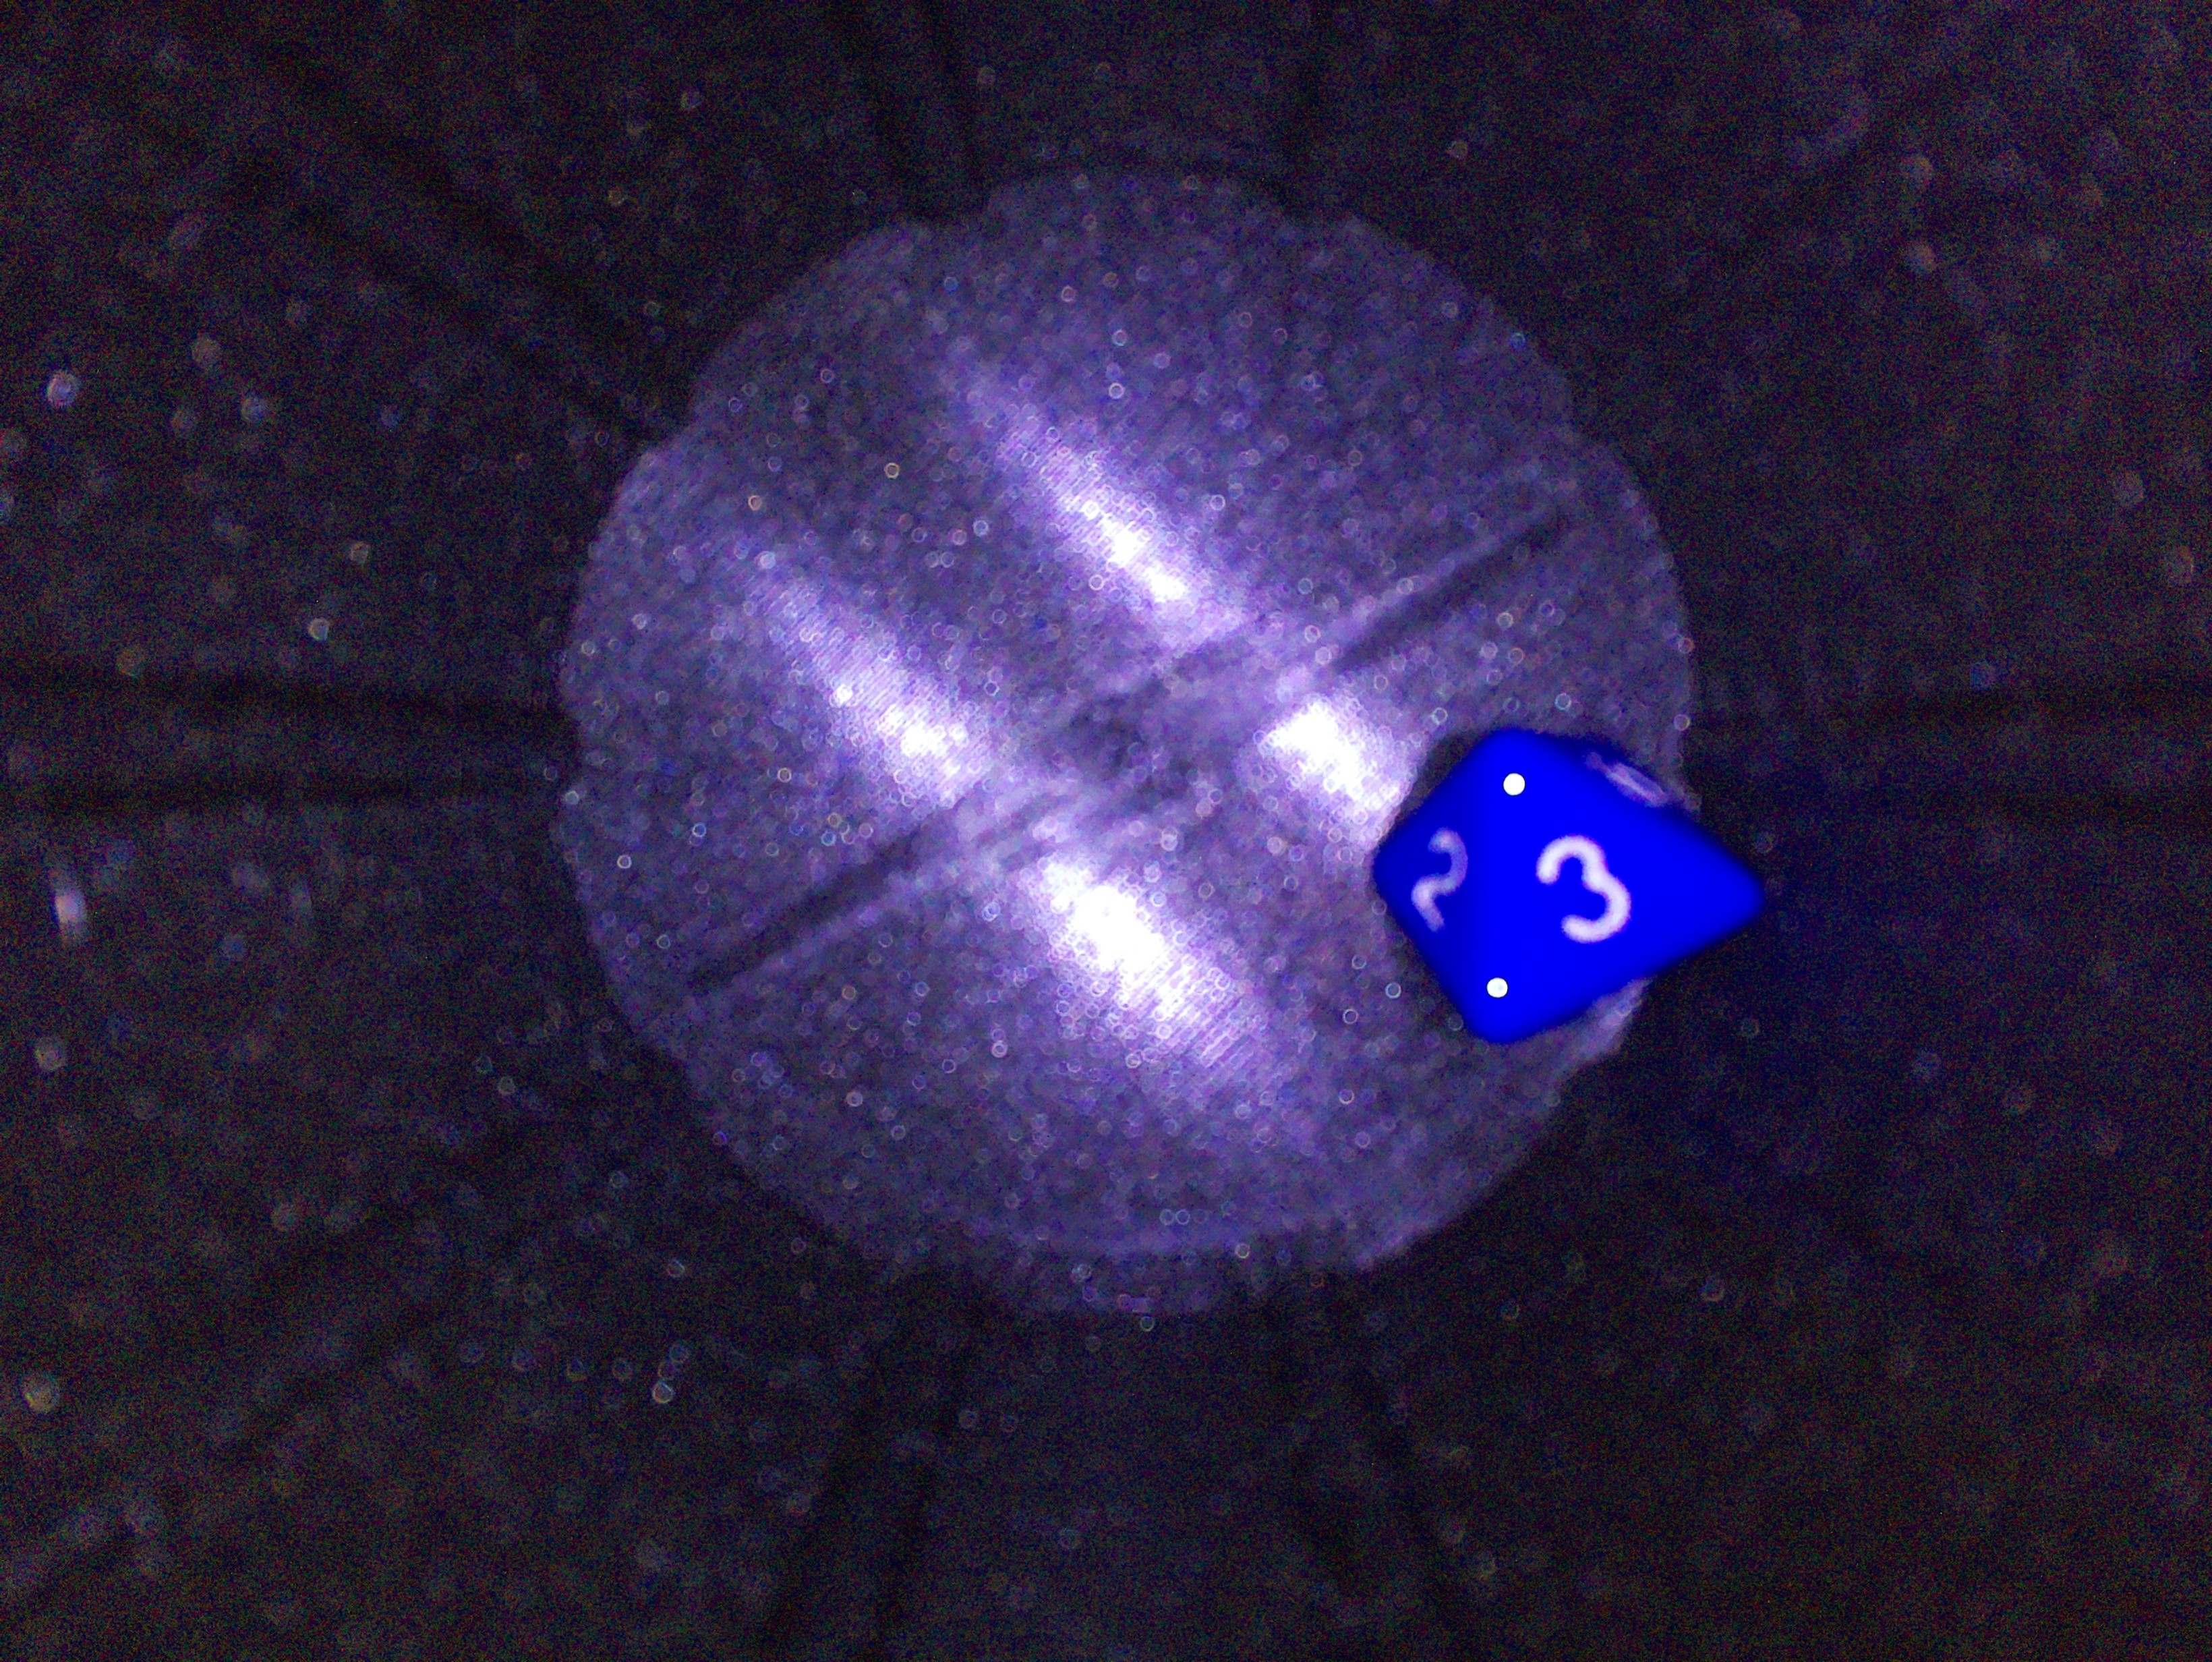
\includegraphics[width=\linewidth]{chapters/03-praca-wlasna/figures/kolorki/niebieska.jpg}
        \caption{\label{fig:blue}Trzecie ustawienie.}
    \end{minipage}
\end{figure}

W obu wariantach dużym problemem był złej jakości obraz z kamery. W tym celu zaprojektowano system oświetlenia składający się z diod
LED sterowanych przy pomocy układu tranzystorów Darlingtona. Dzięki temu wnętrze kubka stało się dużo jaśniejsze, co pozwala kamerze na
robienie zdjęć lepszej jakości. Zdjęcie oświetlonego kubka przedstawiono na rys.~\ref{fig:jasno}. 

Dodatkowo rozświetlenie wnętrza kubka na tyle poprawiło
jakość zdjęć, że pozwoliło to na obniżenie kamery względem kubka. Spowodowało to, że wysokość prototypu zmniejszyła się o około 5cm, 
co było znaczącą poprawą, ponieważ jednym z założeń postawionych na początku budowy było stworzenie urządzenia o niewielkich rozmiarach.
Dzięki tym zabiegom otrzymywane zdjęcia stały się dużo bardziej wyraźne oraz pole widzenia kamery było ograniczone tylko do dna kubka.
Diody LED służące do oświetlenia wnętrza kubka połączono szeregowo. Dzięki temu nie trzeba było wykorzystywać dodatkowych rezystorów a liczba połączeń
jest minimalna, ponieważ wystarczają dwa przewody do podłączenia całego układu diod.

\begin{figure}[H]
    \centering
    \rotatebox{-90}{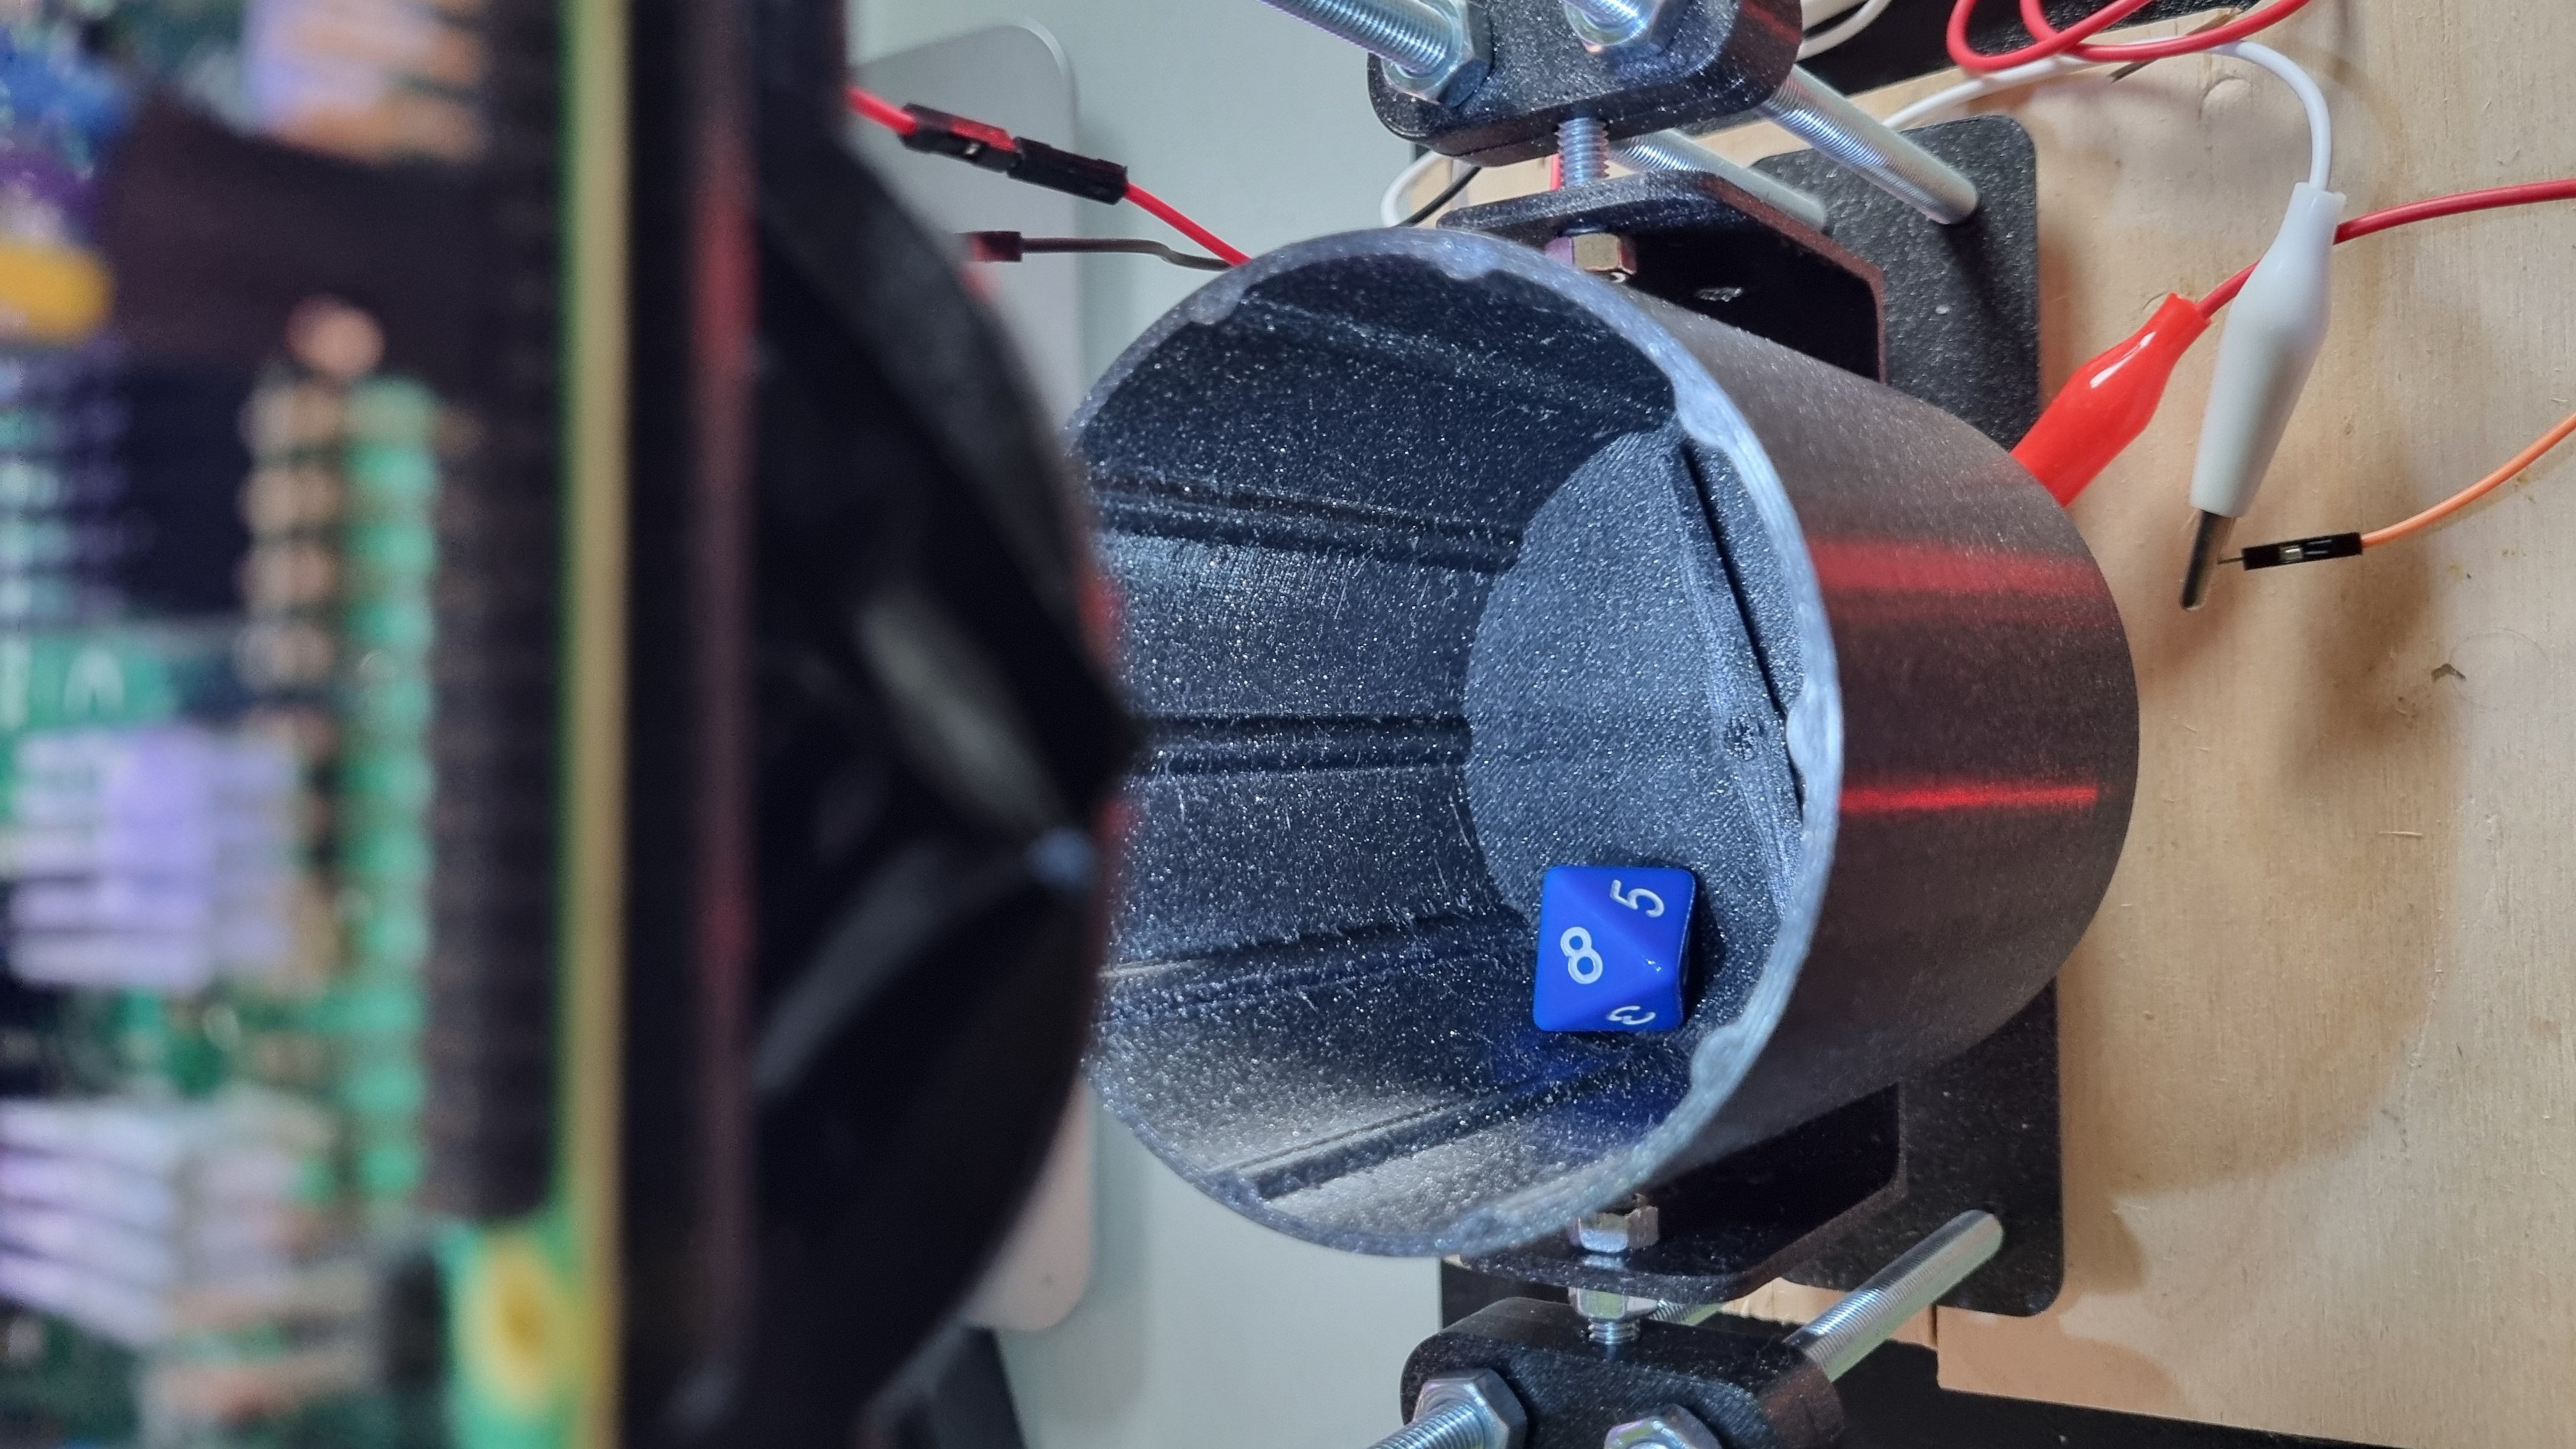
\includegraphics[width=0.45\linewidth]{chapters/03-praca-wlasna/figures/i_stala_sie_jasnosc}}
    \caption{\label{fig:jasno}Oświetlone wnętrze kubka.}
\end{figure}

Podczas testów prototypów konieczne było również określenie wysokości, na której może znajdywać się kamera nad kubkiem. 
%Wysokość tą określono na podstawie jakości zdjęć jako najlepszą podczas testów prototypów. 
W tym celu wykonano zdjęcia z różną odległością kamery od dna kubka (patrz rys.~\ref{fig:wysoko} - \ref{fig:ideolo}). Głównym celem było znalezienie minimalnej odległości kamery od dna kubka, które nie powodowałoby 
znacznego pogorszenia się jakości zdjęć, co utrudniałoby rozpoznawanie wyników na kości. Dodatkową zaletą obniżenia kamery względem kubka był fakt, że kamera
znajdująca się niżej miała w swoim zasięgu widoku tylko dno kubka, co również miało za zadanie ułatwić rozpoznawanie kości oraz jej wartości. W trakcie testowania
odległość tą wyznaczono na 120mm.

\begin{figure}[h]
    \centering
    % Pierwsze zdjęcie
    \begin{minipage}{0.32\textwidth}
        \centering
        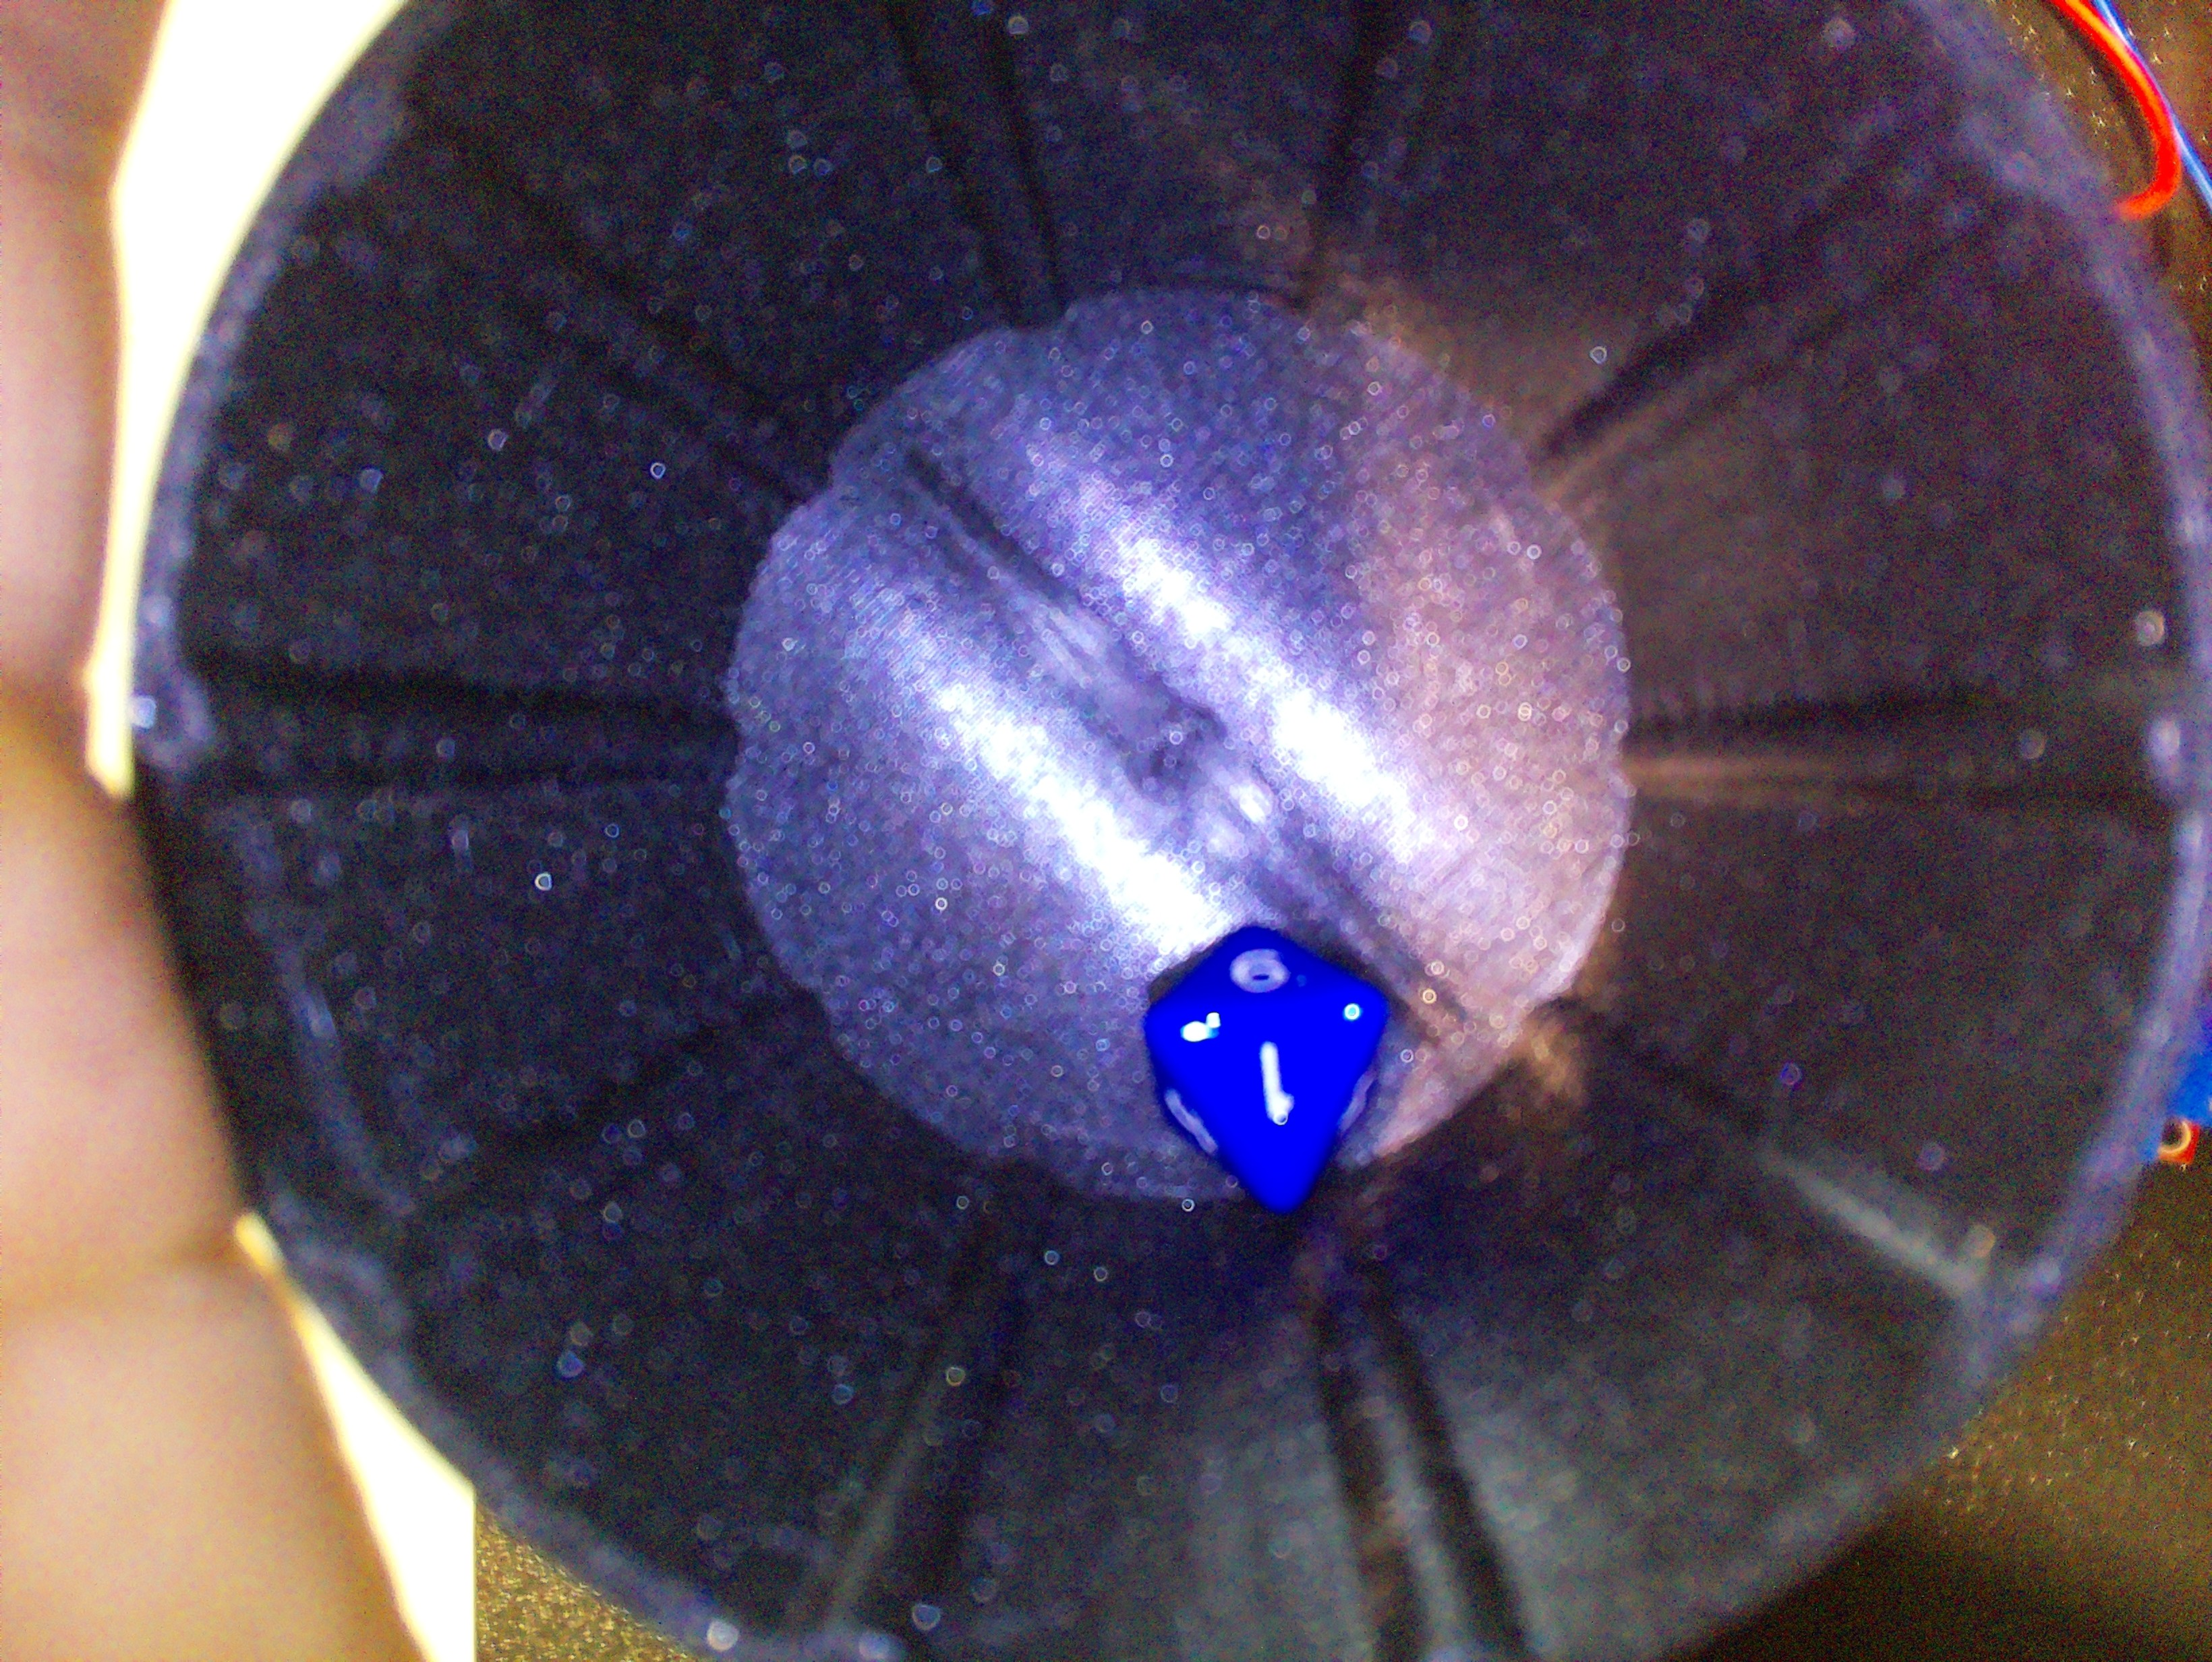
\includegraphics[width=\linewidth]{chapters/03-praca-wlasna/figures/wysoko}
        \caption{\label{fig:wysoko}Pierwsze ustawienie.}
    \end{minipage}
    \hfill
    % Drugie zdjęcie
    \begin{minipage}{0.32\textwidth}
        \centering
        \includegraphics[width=\linewidth]{chapters/03-praca-wlasna/figures/niżej}
        \caption{\label{fig:nizej}Drugie ustawienie.}
    \end{minipage}
    \hfill
    % Trzecie zdjęcie
    \begin{minipage}{0.32\textwidth}
        \centering
        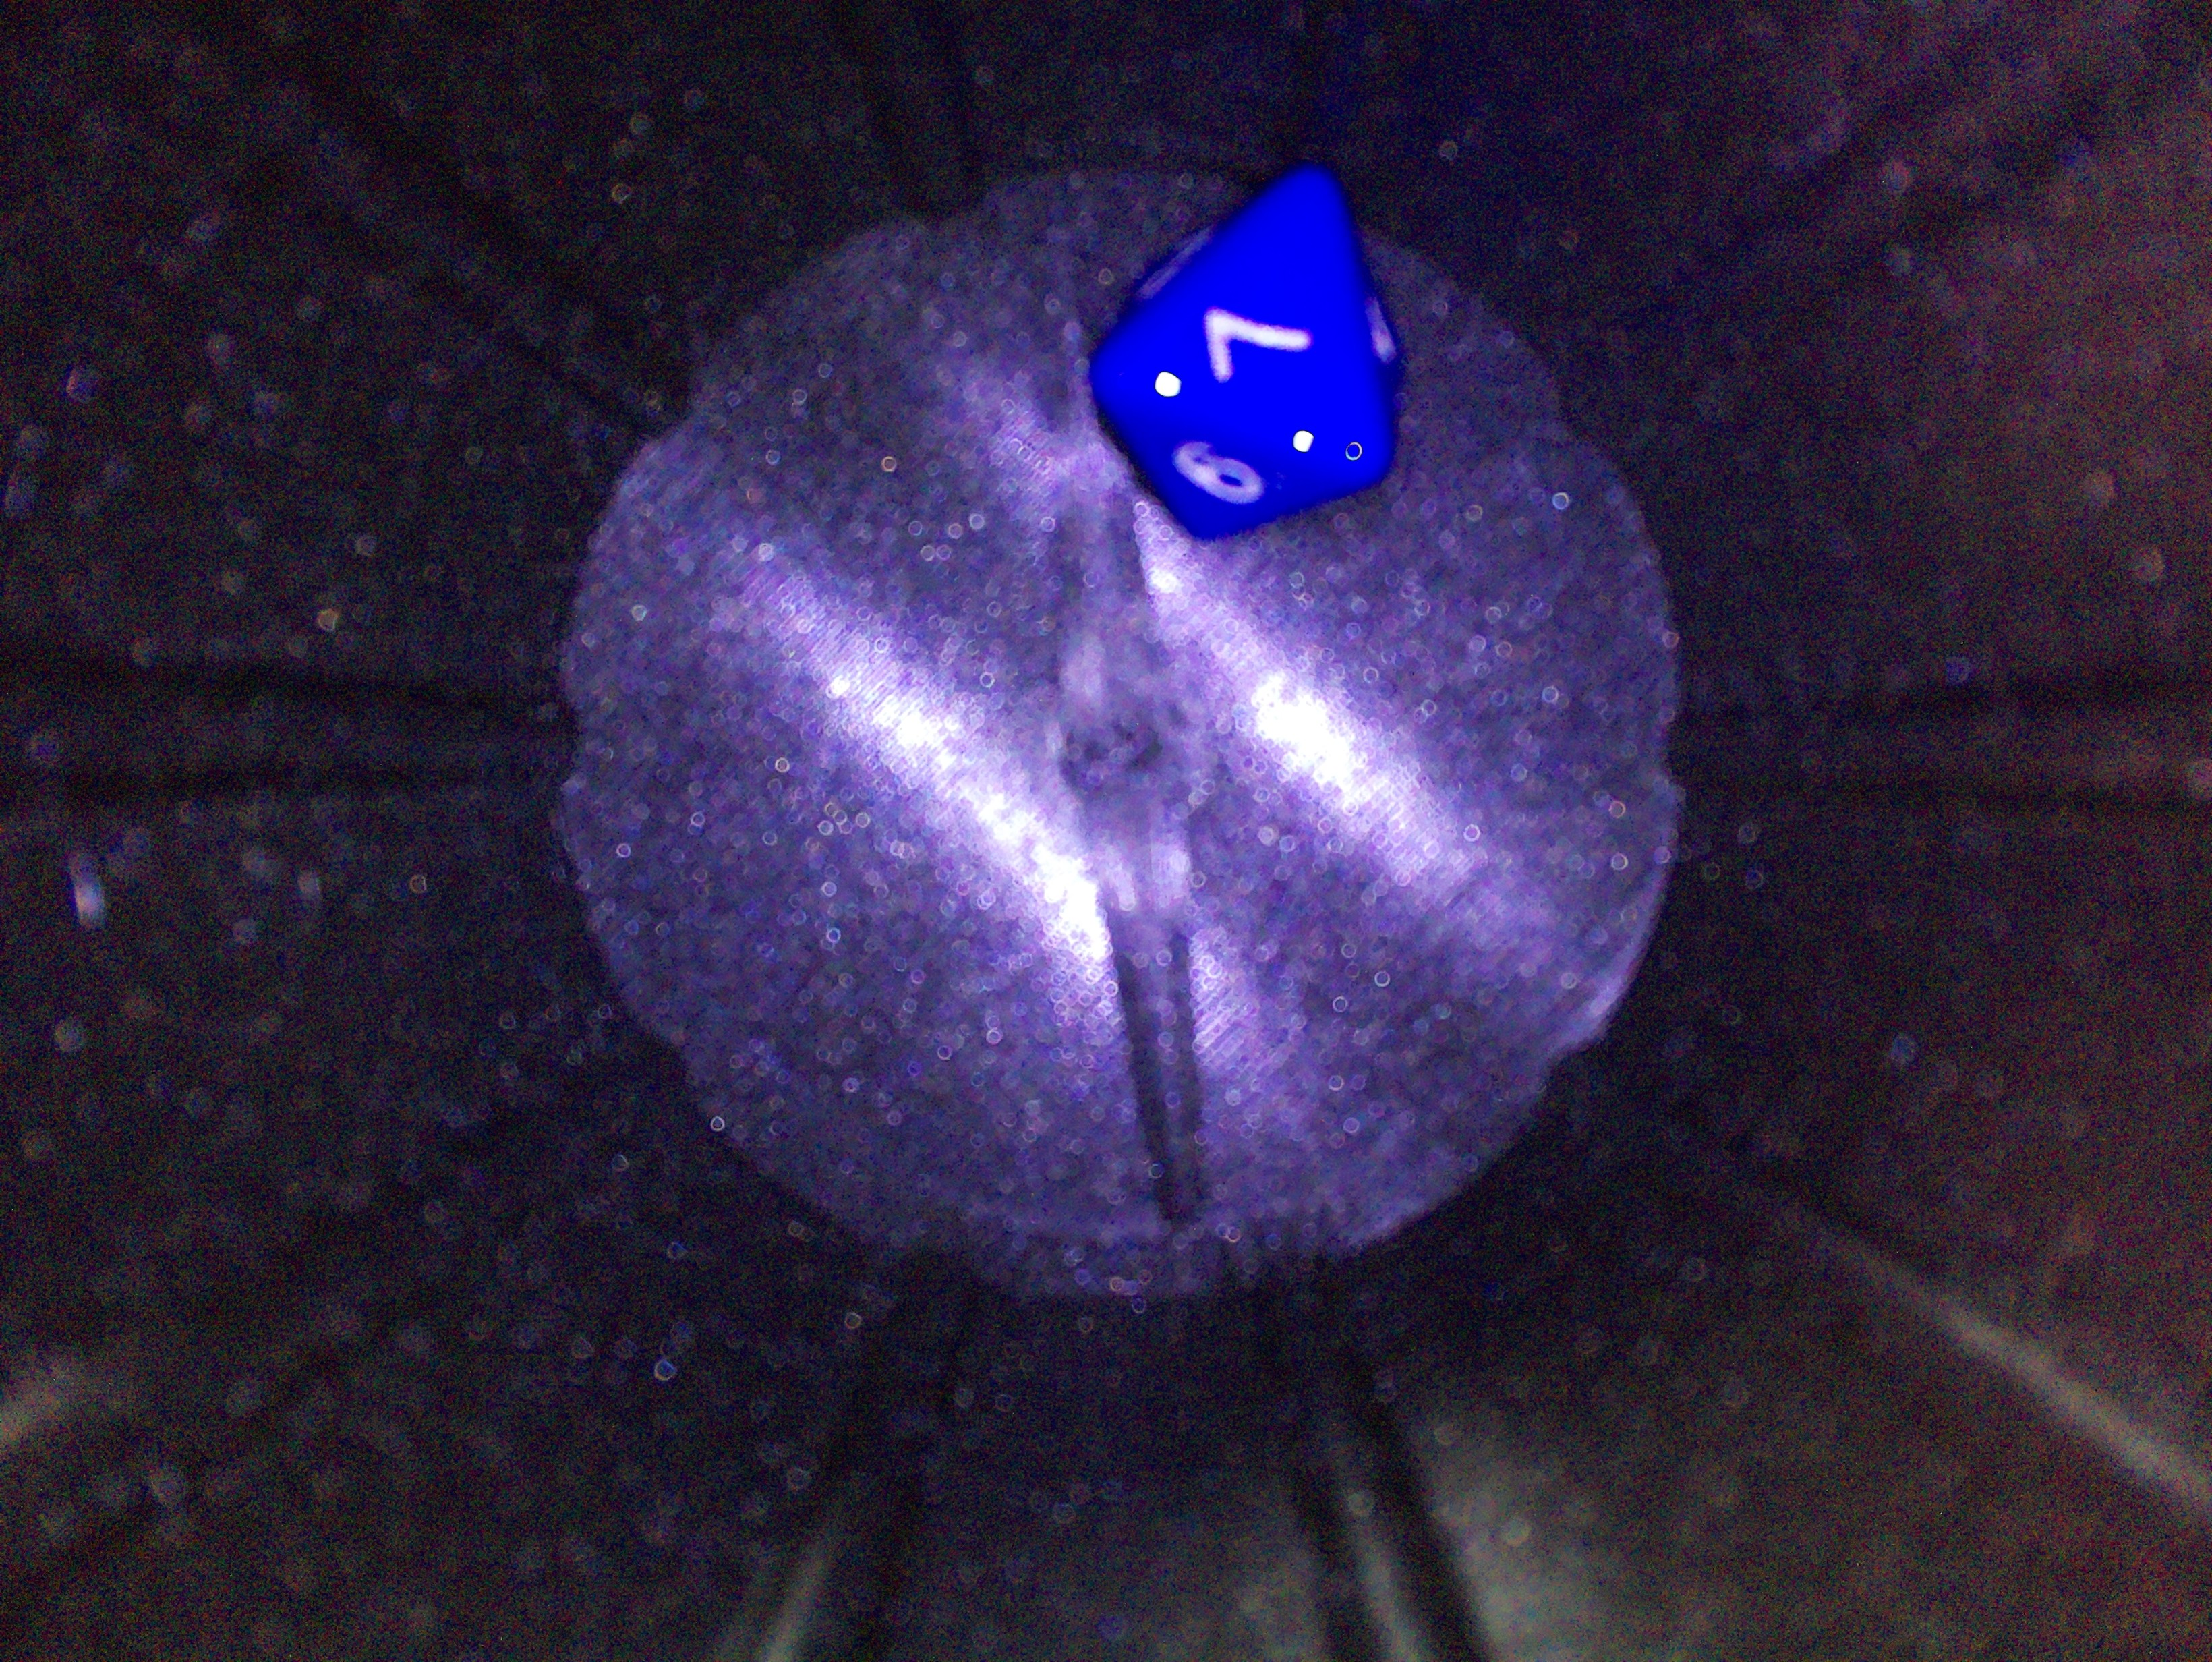
\includegraphics[width=\linewidth]{chapters/03-praca-wlasna/figures/ideolo}
        \caption{\label{fig:ideolo}Trzecie ustawienie.}
    \end{minipage}
\end{figure}

W trakcie testów konieczne okazało się również skorygowanie jasności świecenia diod LED. Wykorzytany układ czterech diod LED połączonych szeregowo dawał zbyt jasne światło, 
co objawiało się poprzez duże odblaski na powierzchni kości, które stanowiły jeden z głównych problemów dla modelu sieci neuronowej odczytującego wyniki rzutów o czym jest mowa
w sekcji \ref{subsec:zidentyfikowane-trudnosci-i-ich-rozwiazania}. Z tego powodu eksperymentalnie wybrano rezystory, których zadaniem było
ograniczenie napięcia zasilającego układ diod LED. Porównanie jasności świecenia układu diod przedstawiono na Rys.~\ref{fig:za jasno} oraz Rys.~\ref{fig:w sam raz}.

\begin{figure}[H]
    \centering
    \begin{minipage}{0.48\textwidth}
        \centering
        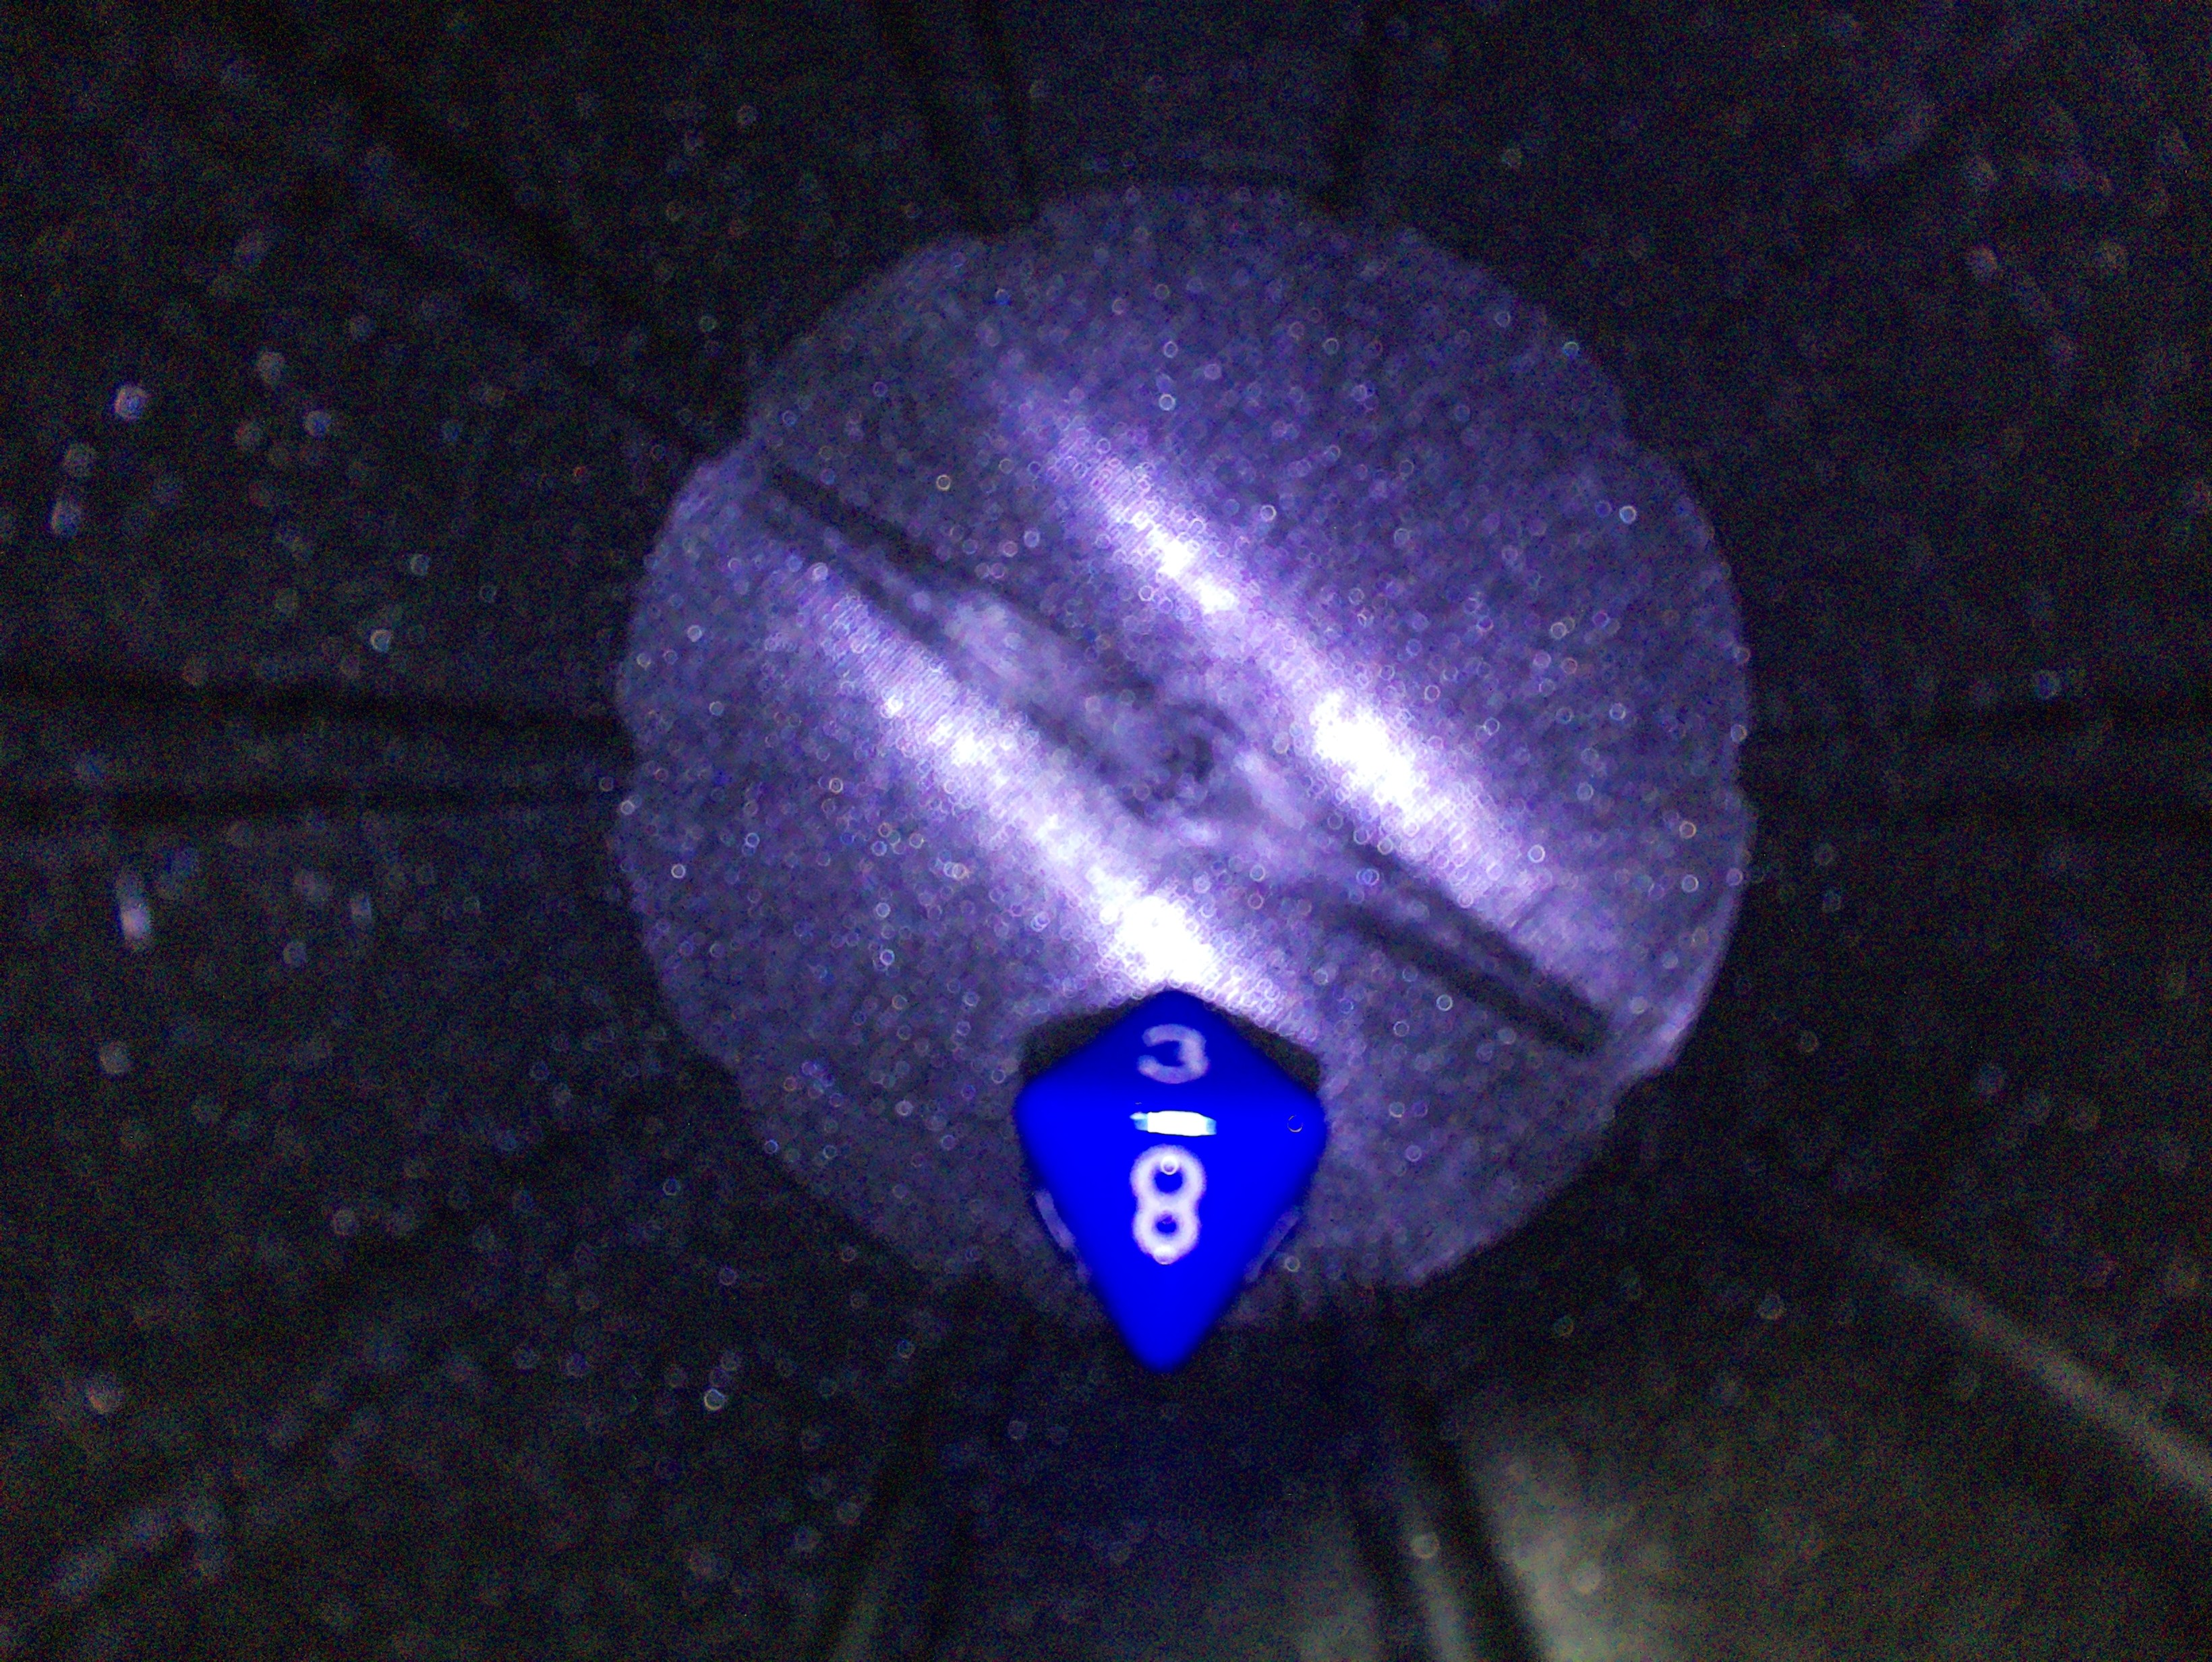
\includegraphics[width=\linewidth]{chapters/03-praca-wlasna/figures/za jasno.jpg}
        \caption{\label{fig:za jasno}Oświetlone wnętrze kubka bez rezystorów ograniczających napięcia zasilającego diody LED.}
    \end{minipage}
    \hfill
    \begin{minipage}{0.48\textwidth}
        \centering
        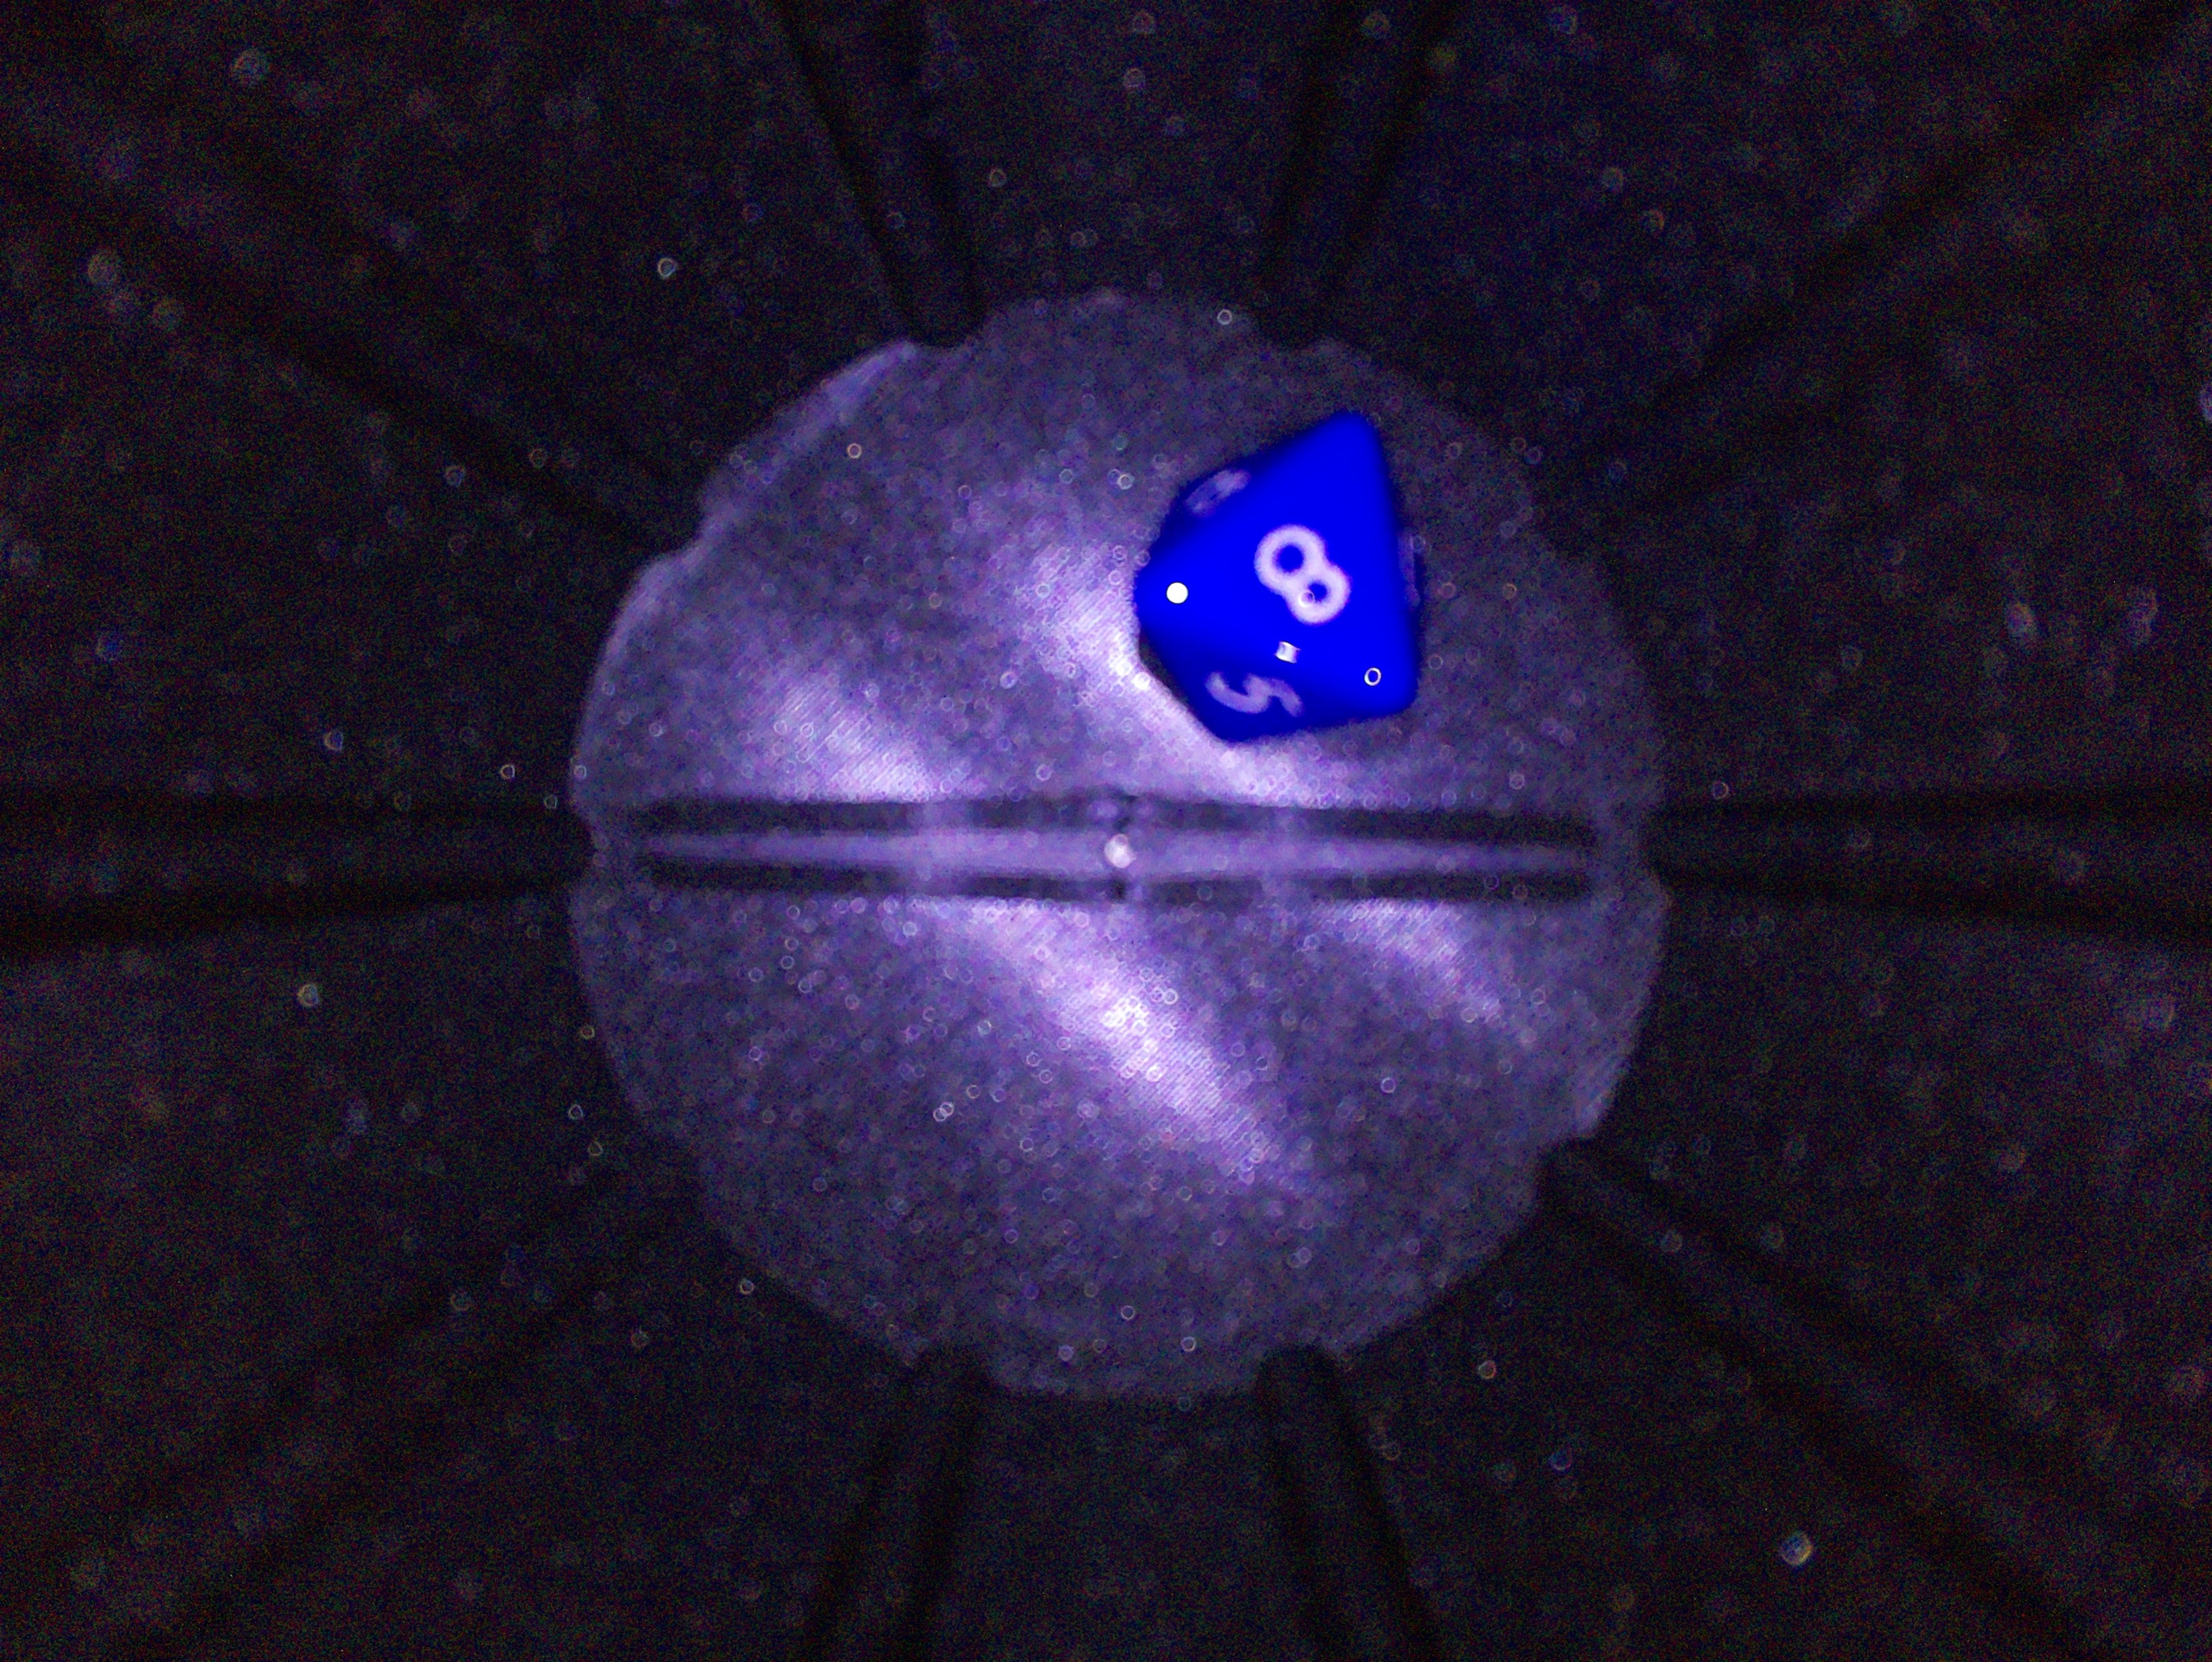
\includegraphics[width=\linewidth]{chapters/03-praca-wlasna/figures/w sam raz.jpg}
        \caption{\label{fig:w sam raz}Oświetlone wnętrze kubka z rezystorami ograniczającymi napięcie zasilające diody LED.}
    \end{minipage}
\end{figure}

Po skonstruowaniu obu wersji robota i wstępnym przetestowaniu ich okazało się, że wariant \textit{blendera} znacznie szybciej (około 4-krotnie) wykonuje rzut kością.
Pojedynczy rzut kością za pomocą \textit{blendera} wraz ze zrobieniem zdjęcia trwa około 1,7 sekundy.
Ponadto wersja \textit{blendera} jest znacznie stabilniejszą konstrukcją, ponieważ nie wymaga poruszania dużymi komponentami robota. 
Największą zaletą wariantu \textit{blendera} jest prostsza -- w porównaniu z wariantem \textit{betoniarki} -- budowa spowodowana mniejszą liczbą ruchomych elementów. Jest to ważne z punktu widzenia
długotrwałej eksploatacji, podczas której bardziej skomplikowane mechanizmy szybciej się zużywają. Z tych powodów do docelowego robota wybrano
wariant \textit{blendera}. Dzięki temu projekt stał się mniej skomplikowany mechanicznie, a jednocześnie jego użyteczność wzrosła, ponieważ
głównym zadaniem tego robota jest generowanie liczb losowych, a to zadanie szybciej był w stanie wykonywać właśnie ten wariant.

%%%%%%%%%%%%%%%%%%%%%%%%%%%%%%%%%%%%%%%%%%%%%%%%%%%%%%%%%%%%%%%%%%%%%%%%%%%%%%%%%%%%%%%%%%%%%%%%%%%%%%%%%%%%%%%%%%%%%%%%%%%%%%%%%%%%%%%%%%%%%%%%%%%%%%

\subsection{Ostateczna wersja robota}\label{subsec:ostateczna-wersja-robota}
Projektowanie ostatecznej wersji robota rozpoczęto od przeanalizowania wad, zalet oraz ogólnych cech prototypów. Postanowiono, że komputer oraz układy sterujące będą
umieszczone z boku kubka, a nie nad nim, tak jak w prototypach, ponieważ sprawiało to, że robot byłby zbyt wysoki względem założenia kompaktowego urządzenia.
Na podstawie testów prototypów wywnioskowano, że najlepszym rozwiązaniem będzie zaprojektowanie obudowy umożliwiającej łatwy dostęp do wszystkich komponentów.
Postanowiono, że finalna wersja robota będzie wykorzystywała kubek o tej samej średnicy co w prototypie. Oznaczało to, że kubek będzie miał zewnętrzną średnicę 80mm
i ścianki o grubości 2 mm, na których tak jak w prototypie będą pionowe żebra (patrz nr 3 na rys.~\ref{fig:kubki}). Dookoła kubka, którego ostateczne wymiary wyniosły 126x80mm,
zaprojektowano resztę konstrukcji. Obudowę zaprojektowano w taki sposób, żeby była w stanie pomieścić kubek oraz kamerę umieszczoną na wysokości 120mm nad dnem kubka.
Dodatkowo w tylnej oraz dolnej części obudowy pozostawiono przestrzeń na resztę
elementów składowych robota. Wielkość tej przestrzeni wyznaczono poprzez zwymiarowanie pozostałych elementów takich jak silnik, sterownik \cite{L298}, wentylator 
czy Raspberry Pi \cite{malina}. Te wymiary posłużyły do określenia minimalnej potrzebnej przestrzeni, którą wyznaczono na około 30mm z tyłu, 35mm od dołu oraz 10mm od góry kubka. To minimum 
zwiększono w taki sposób, żeby we wnętrzu pomieściły się również przewody i śruby oraz żeby po całkowitym złożeniu pozostała przestrzeń do swobodnego manipulowania
elementami składowymi.

Każdy element został zaprojektowany w taki sposób, żeby cały robot był modułowy. Żeby spełnić to założenie, każdy element
zaprojektowano w taki sposób, żeby posiadał on specjalne miejsca na inserty lub śruby. Inserty to mosiężne elementy, które za pomocą lutownicy wgrzewa się
w wydruk 3D. Posiadają one wewnętrzny gwint dzięki czemu można do łączenia wydruków wykorzystywać śruby nie uszkadzając samego wydruku przy 
wielokrotnym skręcaniu i rozkręcaniu robota. Dzięki temu założenie modułowości zostało spełnione, ponieważ dzięki śrubom i insertom każdy element robota 
mógł zostać wydrukowany jako osobna część, którą następnie połączono z innymi częściami w prosty do rozłożenia sposób.

\subsubsection{Opis komponentów ostatecznej wersji robota}

Górna część obudowy, pokrywa przedstawiona na rys.~\ref{fig:pokrywa}, mieszcząca kamerę oraz diody LED, została zaprojektowana w taki sposób, żeby dostęp do kubka pozostał łatwy. Osiągnięto to
poprzez wykorzystanie prostego mocowania pokrywy do obudowy z wykorzystaniem pojedynczej śruby oraz magnesów neodymowych. Dzięki temu w przypadku kiedy konieczny
jest dostęp do kamery lub diod LED, wystarczy zdjąć tylną ścianę robota oraz odkręcić pojedynczą śrubę. Dodatkowo magnesy neodymowe zapewniają
dobre przyleganie pokrywy do reszty obudowy. Ich dodatkową zaletą jest blokowanie pokrywy w ustalonej pozycji podczas umieszczania kości wewnątrz
kubka.

\begin{figure}[H]
    \centering
    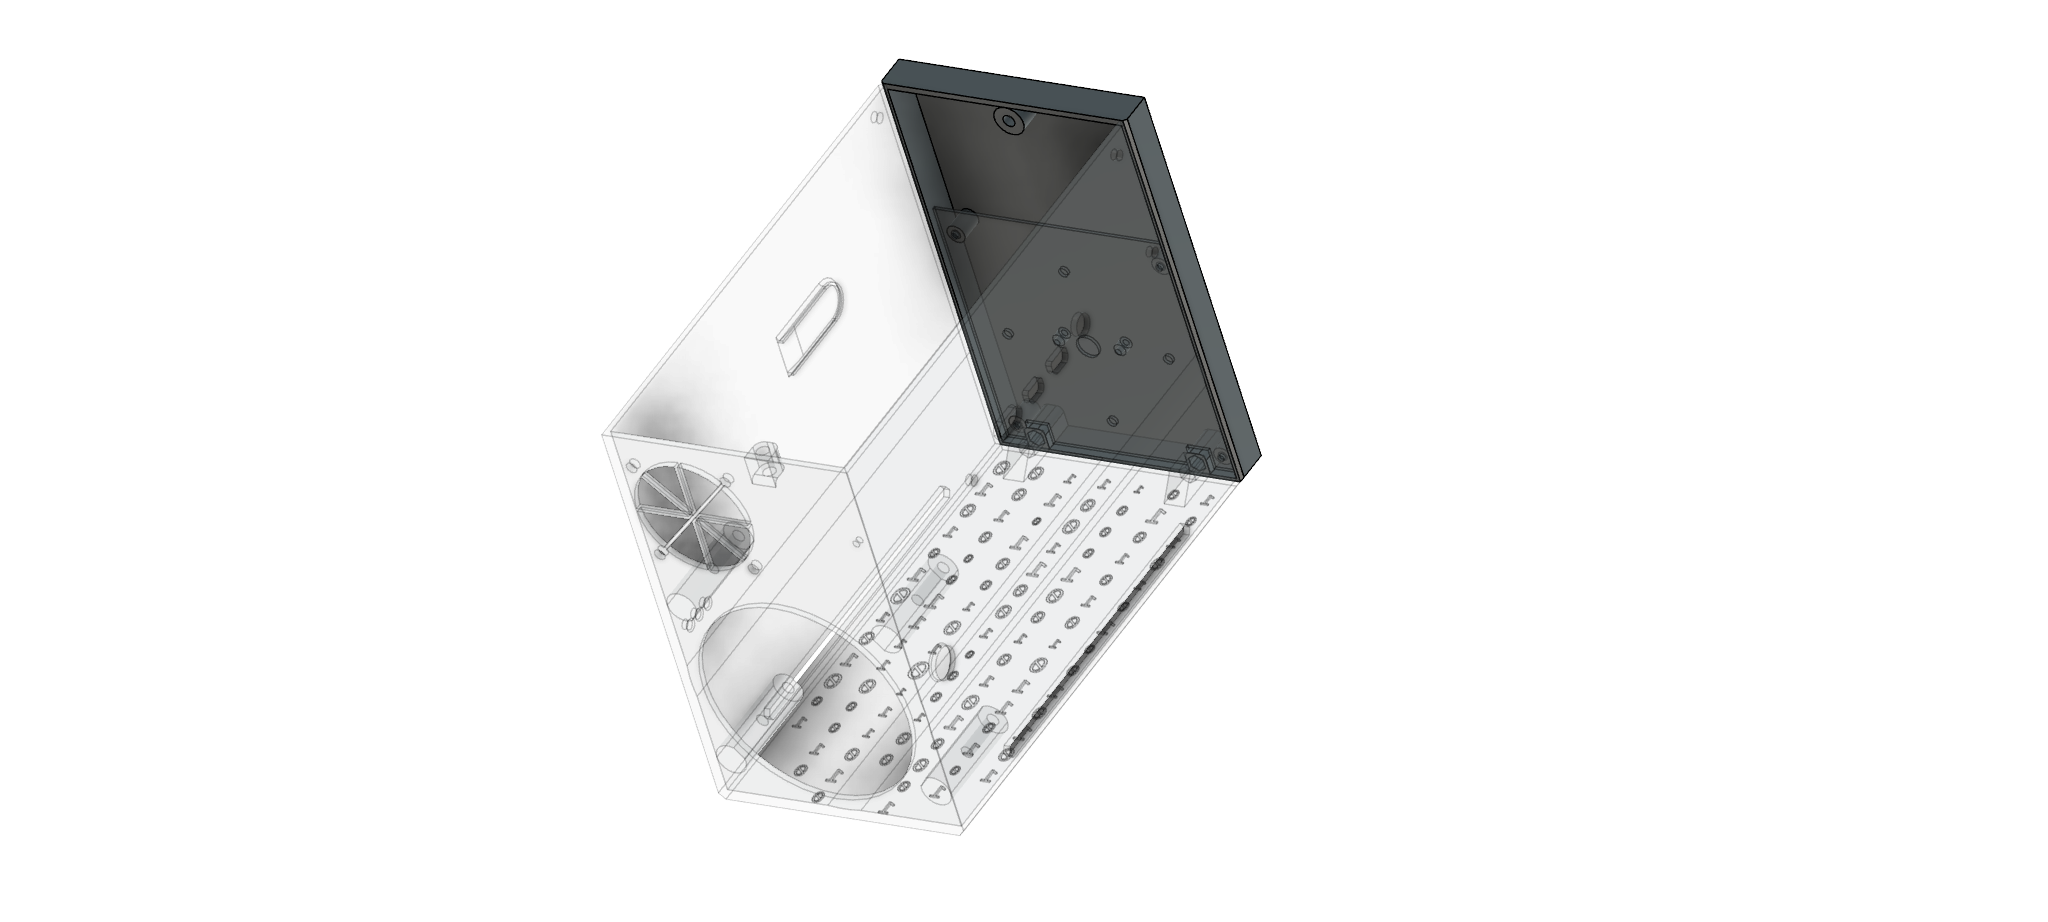
\includegraphics[width=0.95\linewidth]{chapters/03-praca-wlasna/figures/pokrywa}
    \caption{\label{fig:pokrywa}Pokrywa obudowy.}
\end{figure}

Dla zapewnienia sztywności całej konstrukcji oraz punktu mocowania dla tylnej ściany robota zaprojektowano belkę przykręcaną do obu ścian. W tą belkę -- przedstawioną na rys.~\ref{fig:belka} --
wkręcana jest również wcześniej wspominana śruba mocująca pokrywę obudowy.

\begin{figure}[H]
    \centering
    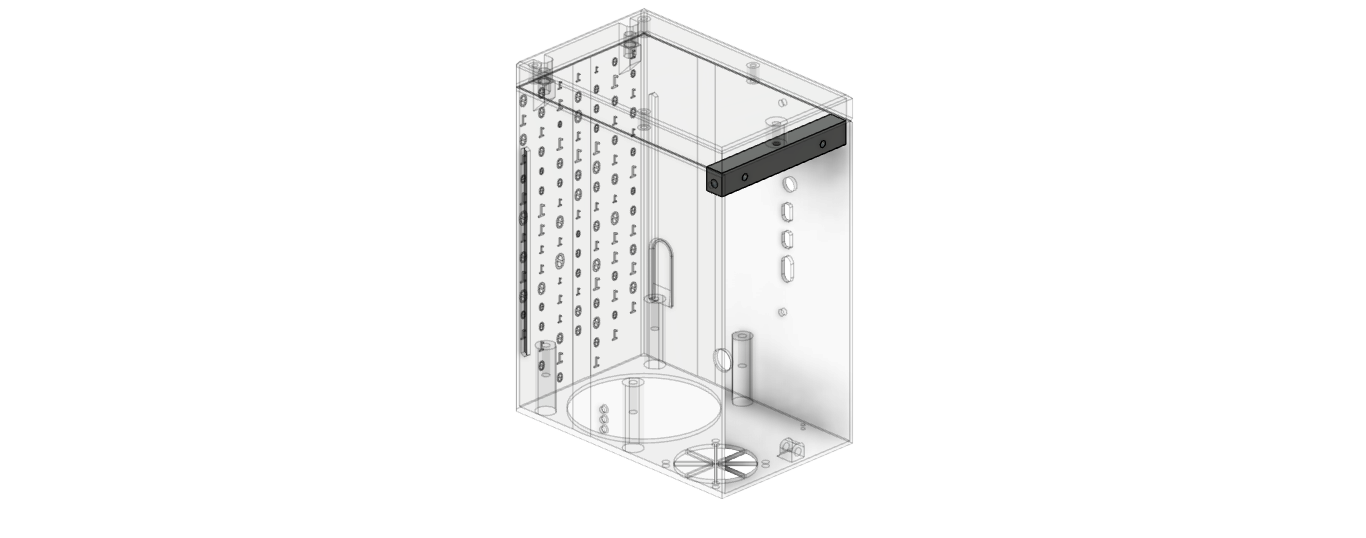
\includegraphics[width=0.95\linewidth]{chapters/03-praca-wlasna/figures/belka}
    \caption{\label{fig:belka}Belka.}
\end{figure}

Kamera wraz z diodami LED służącymi do oświetlenia wnętrza kubka znajduje się w pokrywie. Kamerę zamontowano przy użyciu dwóch śrub M2, natomiast
diody LED umieszczono w zaprojektowanych w wydruku otworach.

W pokrywie znajdują się również dwa sześciokątne otwory na magnesy neodymowe. Dzięki temu, że otwory są sześciokątne, to walcowe magnesy idealnie
się w nie wpasowują i po wciśnięciu nie wypadają. W drugiej części obudowy znajdują się takie same otwory na drugą parę magnesów. Dla pewności podczas umieszczania magnesów 
wykorzystano klej cyjanoakrylowy.

Kubek, w którym dokonywane są rzuty kością, zaprojektowano na podstawie kubka z prototypowej wersji \textit{blendera}. Zachowano jego średnicę oraz kształt i rozmieszczenie wewnętrznych
żeber. Zmieniona została zasada mocowania kubka w taki sposób, żeby był on przystosowany do zamocowania w obudowie. W tym celu zaprojektowano
cztery mocowania widoczne na rys.~\ref{fig:kubek}, znajdujące się u dołu kubka, za pomocą których kubek jest przykręcany do obudowy. Dodatkowo pogrubiono dno kubka tak, żeby można było w nim umieścić inserty służące 
do przykręcenia uchwytu silnika. Ostatnią modyfikacją było podwyższenie kubka w taki sposób, żeby wysokością sięgał on aż do mocowania kamery - górnej pokrywy.
Dzięki temu podczas rzutów zniknął problem z wypadającą kością, co było dość częstym zjawiskiem podczas testów prototypu. Niestety takie rozwiązanie
spowodowało, że wnętrze kubka przestało być widoczne z zewnątrz. Jednak uznano, że widok z zewnątrz na wnętrze kubka nie jest konieczny do osiągnięcia celów projektu.

\begin{figure}[H]
    \centering
    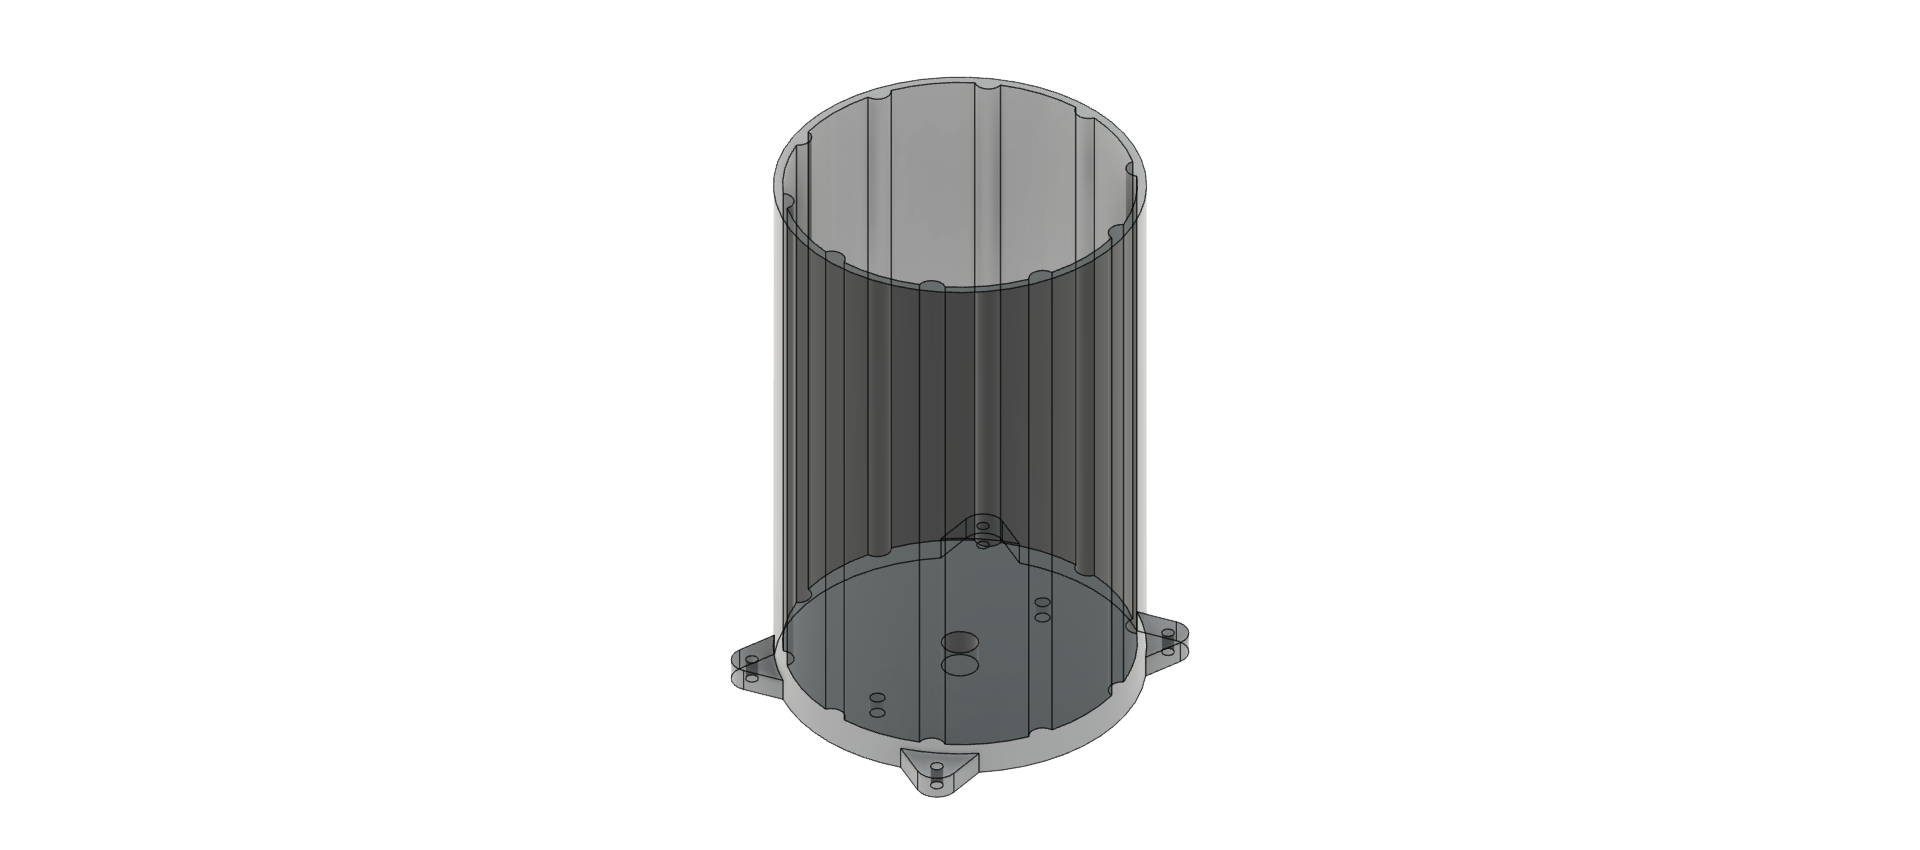
\includegraphics[width=0.95\linewidth]{chapters/03-praca-wlasna/figures/kubek}
    \caption{\label{fig:kubek}Kubek.}
\end{figure}

Projekt pierwszego uchwytu mocującego silnik składał się z miejsca do umieszczenia silnika oraz dwóch cylindrycznych słupków służących za prowadnice
śrub mocujących cały uchwyt do dna kubka. Jednak, ponieważ podczas testów pojawiły się problemy z pierwszym silnikiem i wymieniono go na inny, konieczne
było zaprojektowanie drugiego uchwytu. Podczas projektowania drugiego uchwytu wzorowano sie na projekcie pierwszego, jednak dodano dodatkowy trzeci
cylindryczny słupek na śrubę, która miała służyć do kontrolowania wychylenia całego uchwytu w osi przód-tył. Zwiększyło to możliwość regulacji i w ten sposób
ograniczono tarcie śmigła o dno kubka.

Śmigło zaprojektowano w taki sposób, żeby obracając się przy samym dnie kubka, po uderzeniu w kość wybijało ją w górę. Ten efekt uzyskano
dzięki niskiemu profilowi śmigła oraz bocznych ścian śmigła nachylonych pod kątem $45^{\circ}$.

Podczas testów ostatecznej wersji robota napotkano wcześniej wspominane problemy z pierwotnie wykorzystywanym silnikiem DC 6V. Silnik ten miał okrągły wał przez co śmigło musiało
być bardzo dokładnie spasowane aby uniknąć ślizgania się wału wewnątrz otworu śmigła. To sprawiało, że montowanie śmigła i jego demontaż był bardzo trudny. Dodatkowo po wielokrotnych rzutach kością śmigło
wbijało się coraz niżej na wał silnika i w ostateczności tarło o dno kubka tak mocno, że silnik nie był w stanie się obracać. 
Żeby temu zaradzić, umieszczono pomiędzy śmigłem a dnem kubka metalową podkładkę, po której śmigło mogło się ślizgać łatwiej niż po dnie kubka. To
jednak nie rozwiązało problemu, ponieważ po kolejnych kilku tysiącach rzutów śmigło zaczęło się blokować. 
Z tego powodu postanowiono wymienić silnik na mocniejszy 12V silnik z przekładnią, który ma mniejszą częstotliwość obrotu (około 2000RPM zamiast 4000RPM), ale ma większy moment obrotowy.
Zaletą nowego silnika jest jego wał w kształcie litery „D”. Pozwala to na znacznie luźniejsze spasowanie otworu śmigła z wałem, przez co
demontaż śmigła jest znacznie łatwiejszy. Ponadto nowy silnik jest znacznie cichszy niż poprzedni. Obie wersje uchwytów silnika przedstawiono na rys.~\ref{fig:uchwyt_v1} oraz rys.~\ref{fig:uchwyt_v2}.

\begin{figure}[H]
    \centering
    \begin{minipage}{0.48\textwidth}
        \centering
        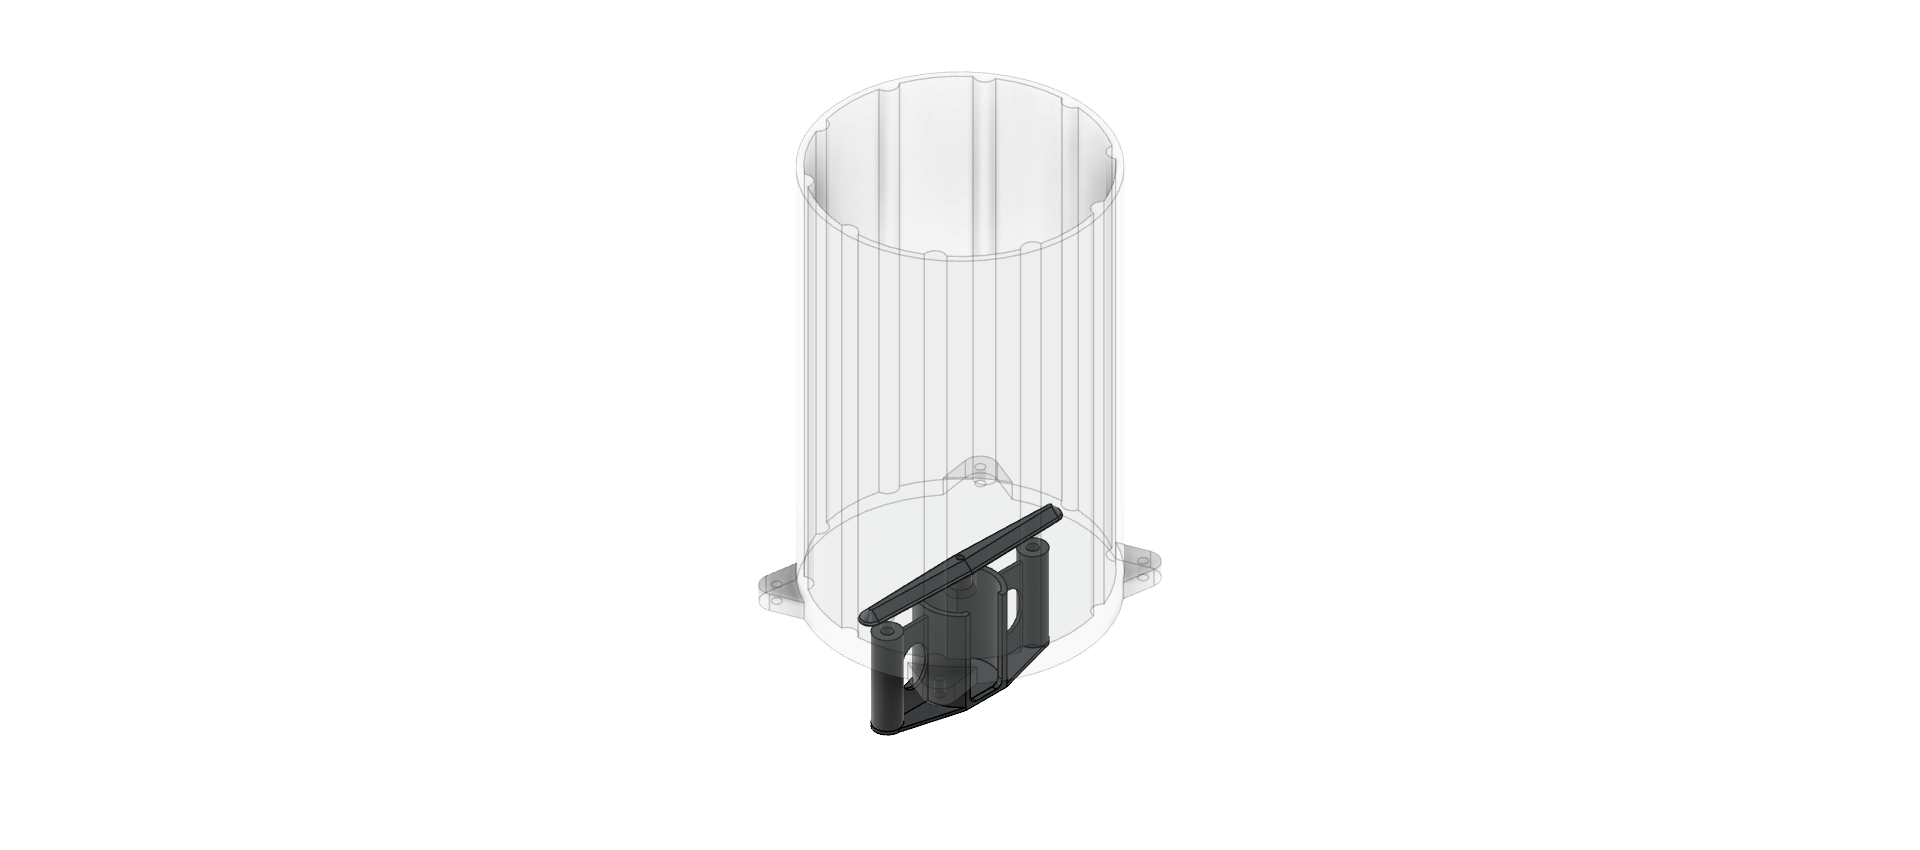
\includegraphics[width=\linewidth]{chapters/03-praca-wlasna/figures/uchwyt_v1}
        \caption{\label{fig:uchwyt_v1}Pierwsza wersja uchwytu silnika oraz śmigło względem kubka.}
    \end{minipage}
    \hfill
    \begin{minipage}{0.48\textwidth}
        \centering
        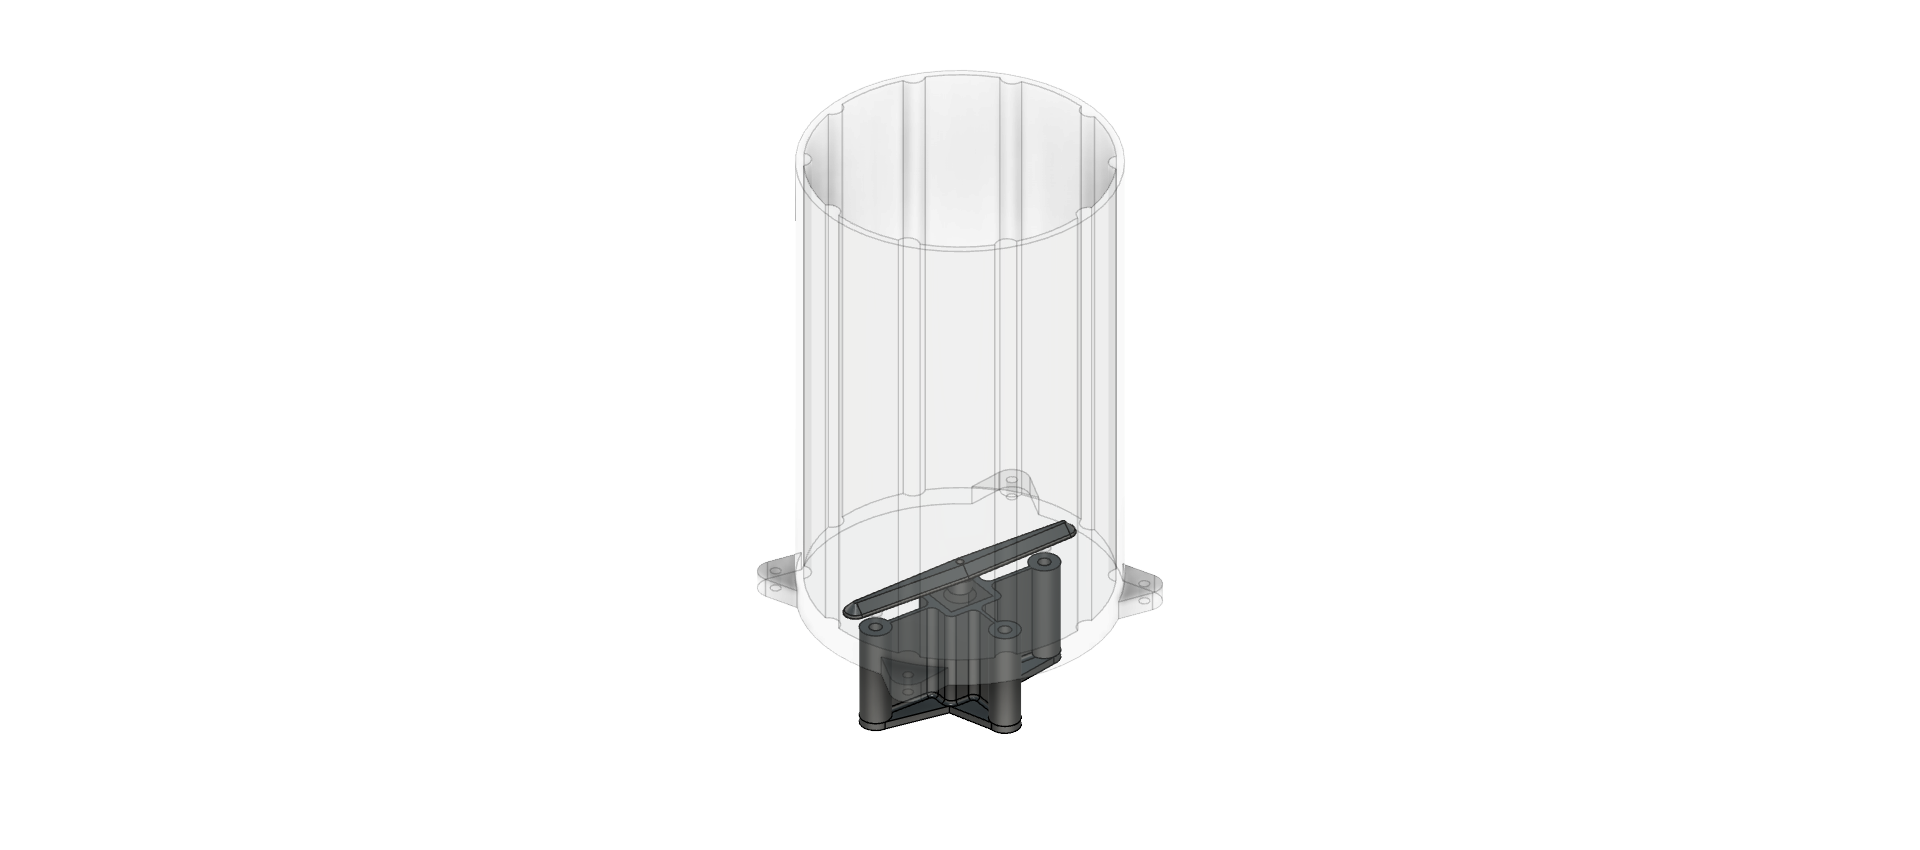
\includegraphics[width=\linewidth]{chapters/03-praca-wlasna/figures/uchwyt_v2}
        \caption{\label{fig:uchwyt_v2}Druga wersja uchwytu silnika oraz śmigło względem kubka.}
    \end{minipage}
\end{figure}


Do mocowania Raspberry Pi zaprojektowano specjalną płytkę przykręcaną do boku obudowy, którą przedstawiono na rys.~\ref{fig:mainboard}. W projekcie tej płytki uwzględniono otwory do przymocowania Raspberry
Pi oraz układu ULN2803A Darlington. Dodatkowo przygotowano specjalne miejsce do mocowania przycisku. Na płytce pozostawiono również miejsce
na zamontowanie szyny zasilania. Płytkę tą umieszczono w obudowie w taki sposób, żeby znajdowała się ona bezpośrednio nad wentylatorem. Dzięki temu
strumień powietrza bezpośrednio chłodzi najważniejsze elementy elektroniczne robota. Przycisk zamocowano na tej samej płytce, z wykorzystaniem
dodatkowego elementu wydrukowanego na drukarce 3D. Dzięki temu znalazł się on bezpośrednio przy ściance obudowy, a dodatkowo jego mocowanie
nadal spełnia założenie modułowości poprzez mocowanie za pomocą śrub i insertów.

\begin{figure}[H]
    \centering
    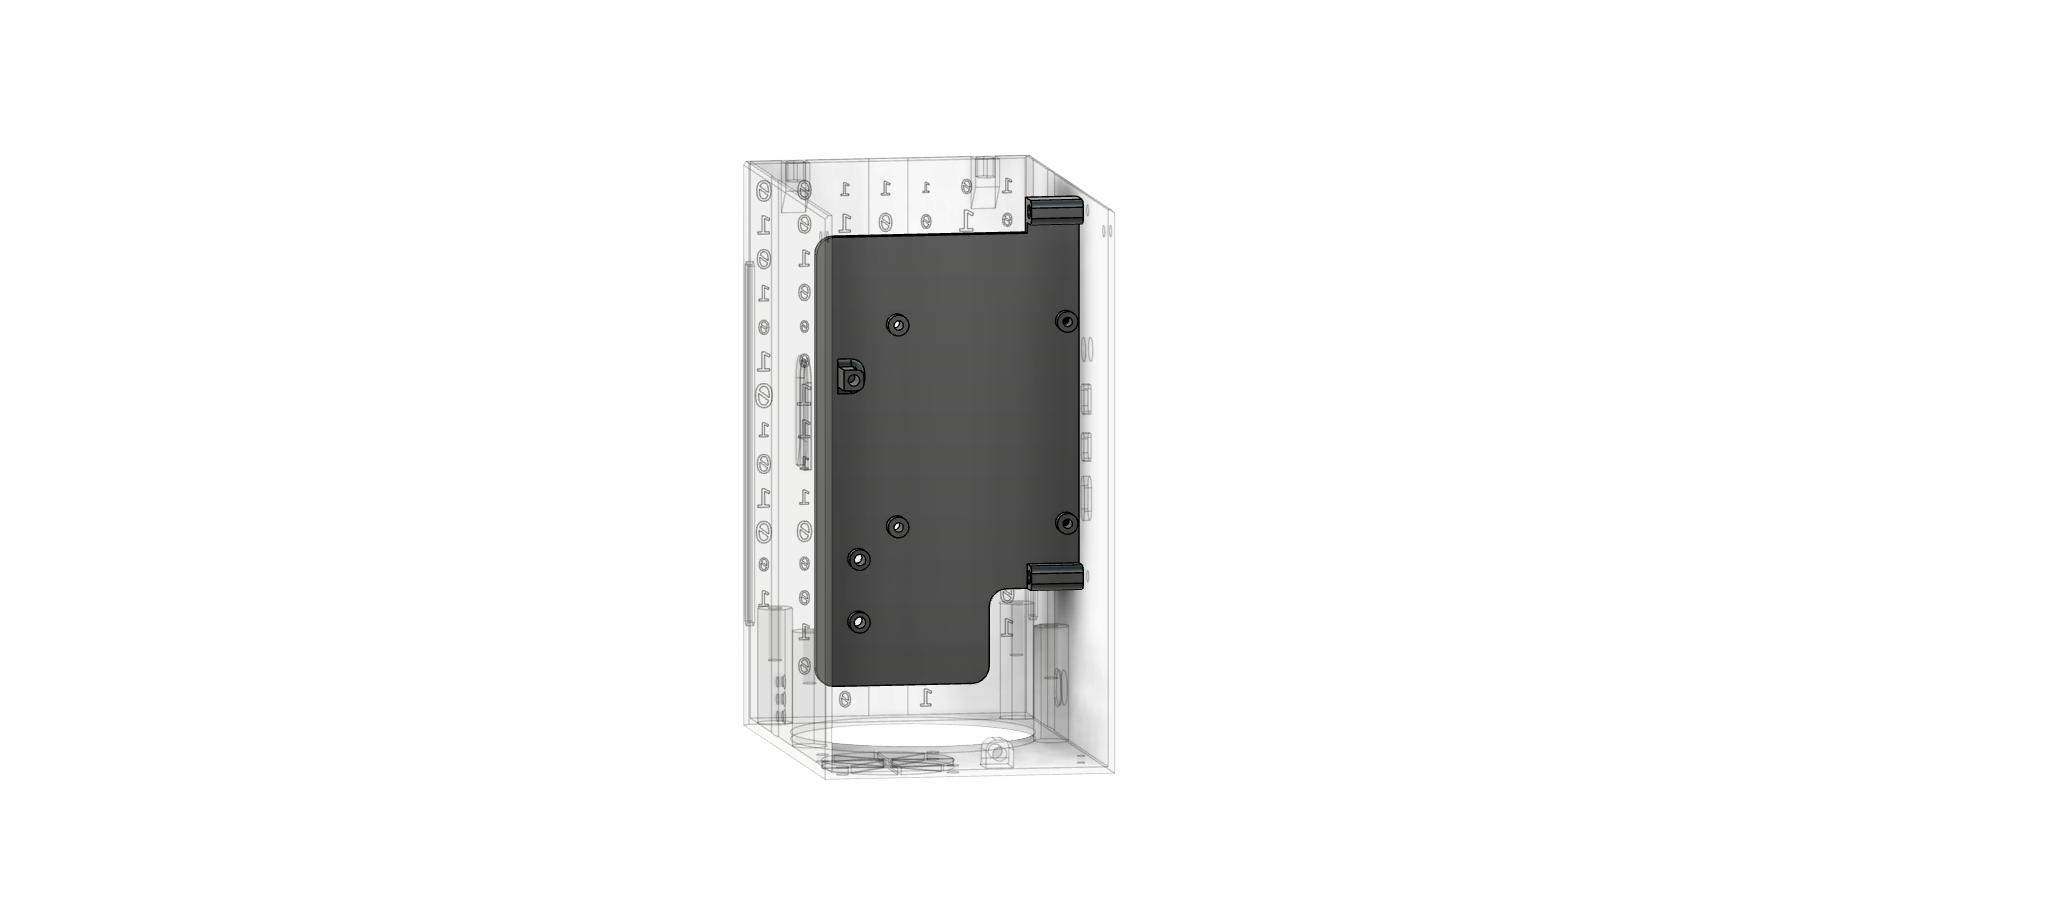
\includegraphics[width=0.95\linewidth]{chapters/03-praca-wlasna/figures/main_board}
    \caption{\label{fig:mainboard}Płytka do montażu elektroniki.}
\end{figure}

Układ sterujący silnikiem L298 przykręcono do obudowy pośrednio, poprzez specjalnie zaprojektowane i wydrukowane mocowanie. Dzięki temu wykorzystano
gotowe otwory na śruby znajdujące się w płytce układu L298. Na rys.~\ref{fig:steownik}, na którym przedstawiono płytkę do mocowania elektroniki
z zamontowaną Raspberry Pi 4b oraz układ L298, widoczne jest wspominane mocowanie służące do przykręcenia układu L298 do dna obudowy robota.

\begin{figure}[H]
    \centering
    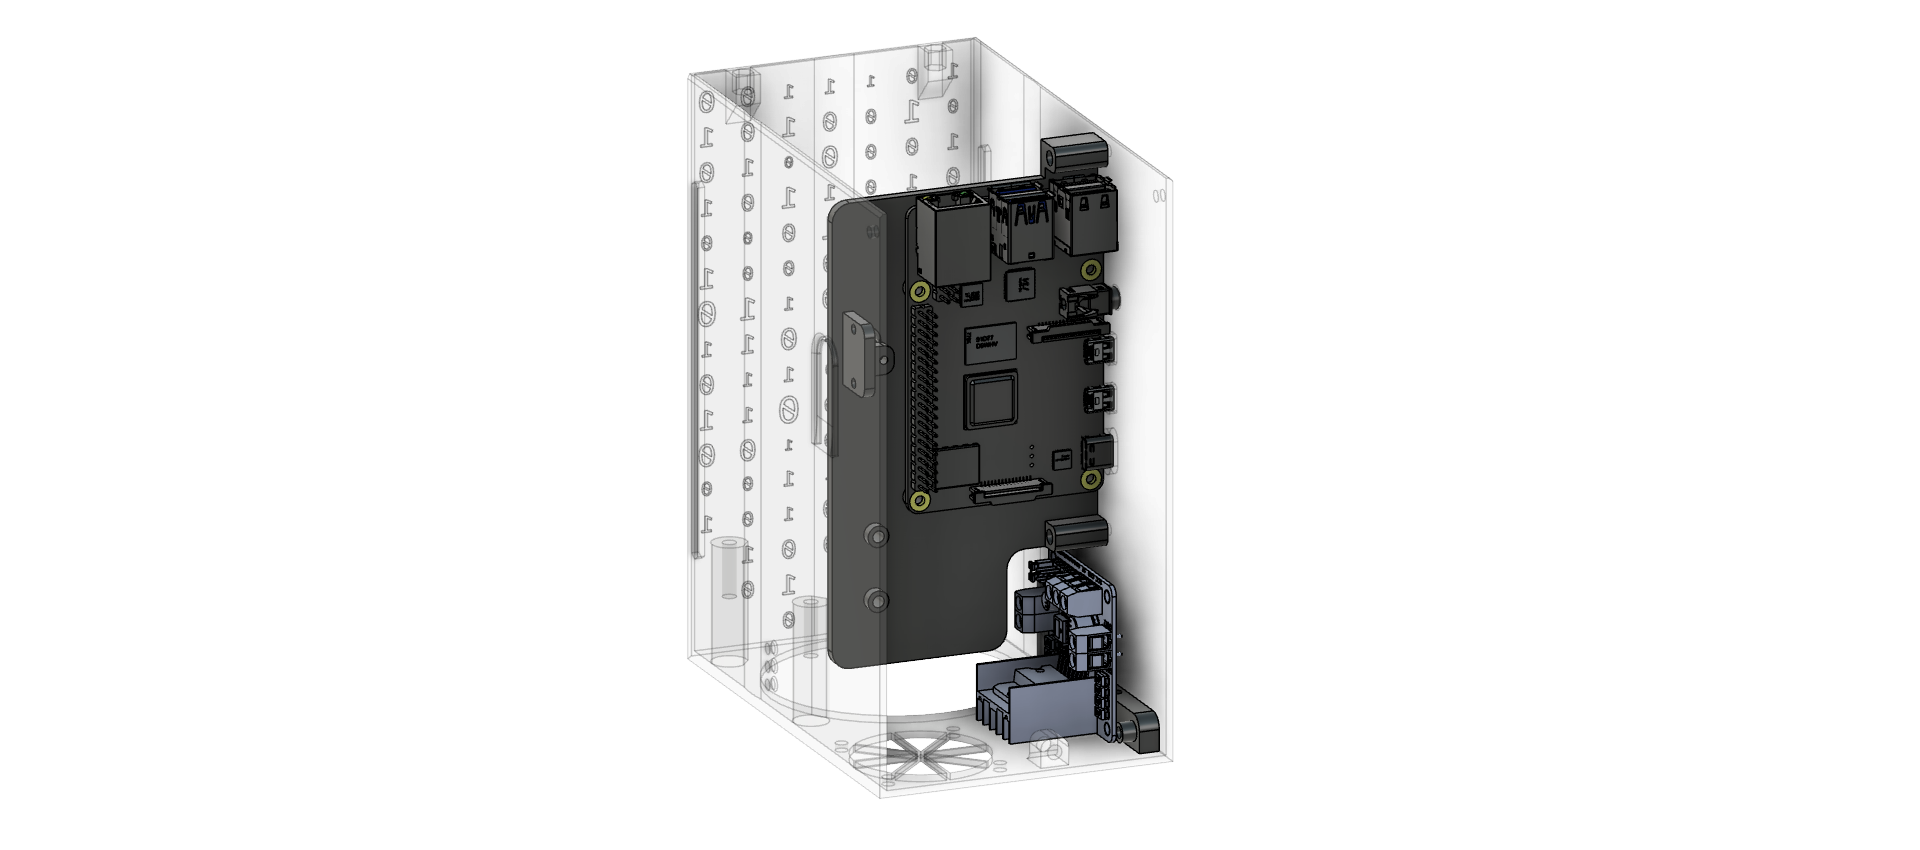
\includegraphics[width=0.95\linewidth]{chapters/03-praca-wlasna/figures/l298n}
    \caption{\label{fig:steownik}Zamocowany sterownik L298 \cite{L298n3d} z widoczną płytką, na której zamocowana jest Raspberry Pi 4b \cite{malina3d}.}
\end{figure}

Do dna obudowy robota przymocowano, za pomocą śrub, również wentylator.

Obudowę zaprojektowano w taki sposób, żeby pomieściła wszystkie powyższe elementy. W jej ścianach zaprojektowano otwory na wyjścia Raspberry Pi,
diody LED oraz gniazdo zasilania. W ścianie obudowy na wysokości miejsca, w którym znajduje się wewnątrz przycisk, zaprojektowano specjalne wycięcie.
Dzięki dodatkowemu zmniejszeniu grubości ściana obudowy w tym miejscu jest bardziej elastyczna, co pozwala na kliknięcie przycisku znajdującego
się po wewnętrznej stronie ściany obudowy. Na dnie obudowy zaprojektowano również specjalne słupki służące za podpórki dla kubka.
W słupkach tych zaprojektowano otwory na inserty, dzięki którym kubek można przykręcić do obudowy gwarantując tym jego stabilność.

Podczas projektowania obudowy przewidziano także takie elementy jak wycięcia od spodu bezpośrednio pod wentylatorem, służące za wlot powietrza
oraz wycięcia w tylnej ściance, służące za wylot powietrza. Dodatkowo w dnie umieszczono duży utwór umożliwiający swobodne mocowanie oraz dostęp do
silnika, diod LED oraz gniazda zasilania. Na bocznych ścianach zaprojektowano przerwy, które następnie zaślepiono kontrastującym kolorystycznie filamentem.
Przerwy te tak samo jak cyfry na przedniej ścianie obudowy są tylko i wyłącznie elementami estetycznymi. Ostatnim elementem robota są zaprojektowane nóżki,
które przyklejono do dna robota. Zapewniają one przepływ powietrza pod robotem gdzie znajduje się wlot powietrza do wentylatora. Gotowy model robota przedstawiono
na rys.~\ref{fig:gotowy} oraz rys.~\ref{fig:srodek}.

\begin{figure}[H]
    \centering
    
\includegraphics[width=0.95\linewidth]{chapters/03-praca-wlasna/figures/gotowy2}
    \caption{\label{fig:gotowy}Projekt gotowego robota od frontu.}
\end{figure}

\begin{figure}[H]
    \centering
    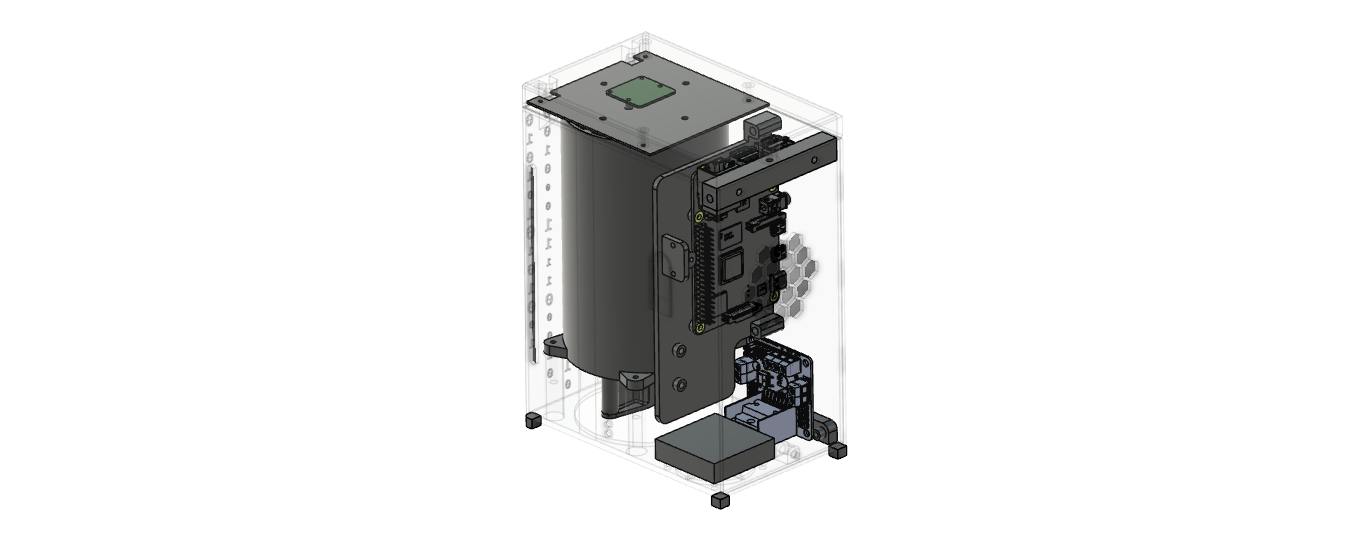
\includegraphics[width=0.95\linewidth]{chapters/03-praca-wlasna/figures/gotowy w srodku}
    \caption{\label{fig:srodek}Projekt gotowego robota z pokazanymi wewnętrznymi komponentami.}
\end{figure}
\section{Dokumentacja techniczna}
\subsection{Hardware}
\subsubsection{Ogólne parametry robota:}
Wymiary: 

Waga:

\subsubsection{Komponenty:}
Elektronika:
    \begin{itemize}
        \item Raspberry Pi 4B,
        \item Raspberry Pi Camera V2,
        \item LN298,
        \item ULN2803A Darlington,
        \item silnik DC 12V,
        \item diody LED 3mm,
        \item przycisk monostabliny THT.
    \end{itemize}

Elementy strukturalne (Wydrukowane na drukarce 3D. Materiał, którego użyto to PLA):
    \begin{itemize}
        \item obudowa,
        \item tylna ściana obudowy,
        \item górna pokrywa,
        \item płytka do montażu kamery i diod LED,
        \item uchwyt do silnika,
        \item płytka do montażu elektroniki,
        \item śmigło.
    \end{itemize}\

Zasilanie:
Zasilacz DC 12V.

\subsubsection{Diagramy i schematy:}








\subsection{Software}
bbbbbbbbbbbbbbbbbbbbb
\chapter{Odczytywanie losowego wyniku z kości}\label{ch:odczytywanie-losowego-wyniku-z-kosci}

Kolejnym krokiem przetwarzania jest odczyt wylosowanej wartości z kości.
Jak pokazano na rys.~\ref{fig:schemat_workflow}
najpierw zdjęcie musi zostać poddane odpowiedniemu przetwarzaniu, które zostało opisane w tym rozdziale.

\begin{figure}[H]
    \centering
    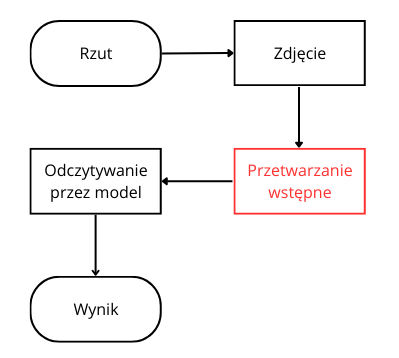
\includegraphics[width=0.5\linewidth]{chapters/04-czytanie/figures/schemat}
    \caption{Ten schemat jest do zmiany na ładniejszy, ale ja nie umiem rys. więc jest taki "na teraz"}
    \label{fig:schemat_workflow}
\end{figure}

\section{Przetwarzanie wstępne obrazów}\label{sec:preprocessing}

W niniejszym rozdziale omówiono proces przetwarzania wstępnego obrazów kości,
który przekształca dane pochodzące z fizycznego komponentu robota (kamery dostarczającej zdjęcia kości) na dane wejściowe dla modelu sztucznej inteligencji.
Przez dane wejściowe dla modelu SI rozumie się tutaj odpowiednio sformatowane obrazy, a więc takie w skali szarości,
o rozmiarach 64x64 piksele, zawierające jedynie kość wyciętą ze zdjęcia (nie zawierające w tle całego kubka).

\subsection{Algorytm}\label{subsec:algorytm}

\begin{enumerate}
    \item Wczytanie obrazu wejściowego .
    \item Odnalezienie kości za pomocą maski na komponencie nasycenia.
    \item Stworzenie i wycięcie ramki ograniczającej (ang. \textit{bounding box}) wokół maski.
    \item Przeskalowanie do odpowiedniego rozmiaru.
    \item Konwersja do skali szarości.
    \item Zapisanie gotowego obrazu.
\end{enumerate}

Na rys.~\ref{fig:preproc_steps} przedstawiono przykładowe zdjęcie surowe~\ref{fig:step1}
oraz kolejne etapy przetwarzania, aż do finalnego etapu~\ref{fig:step5}.

\begin{figure}[H]
    \centering
    \begin{subfigure}[t]{0.32\linewidth}
        \centering
        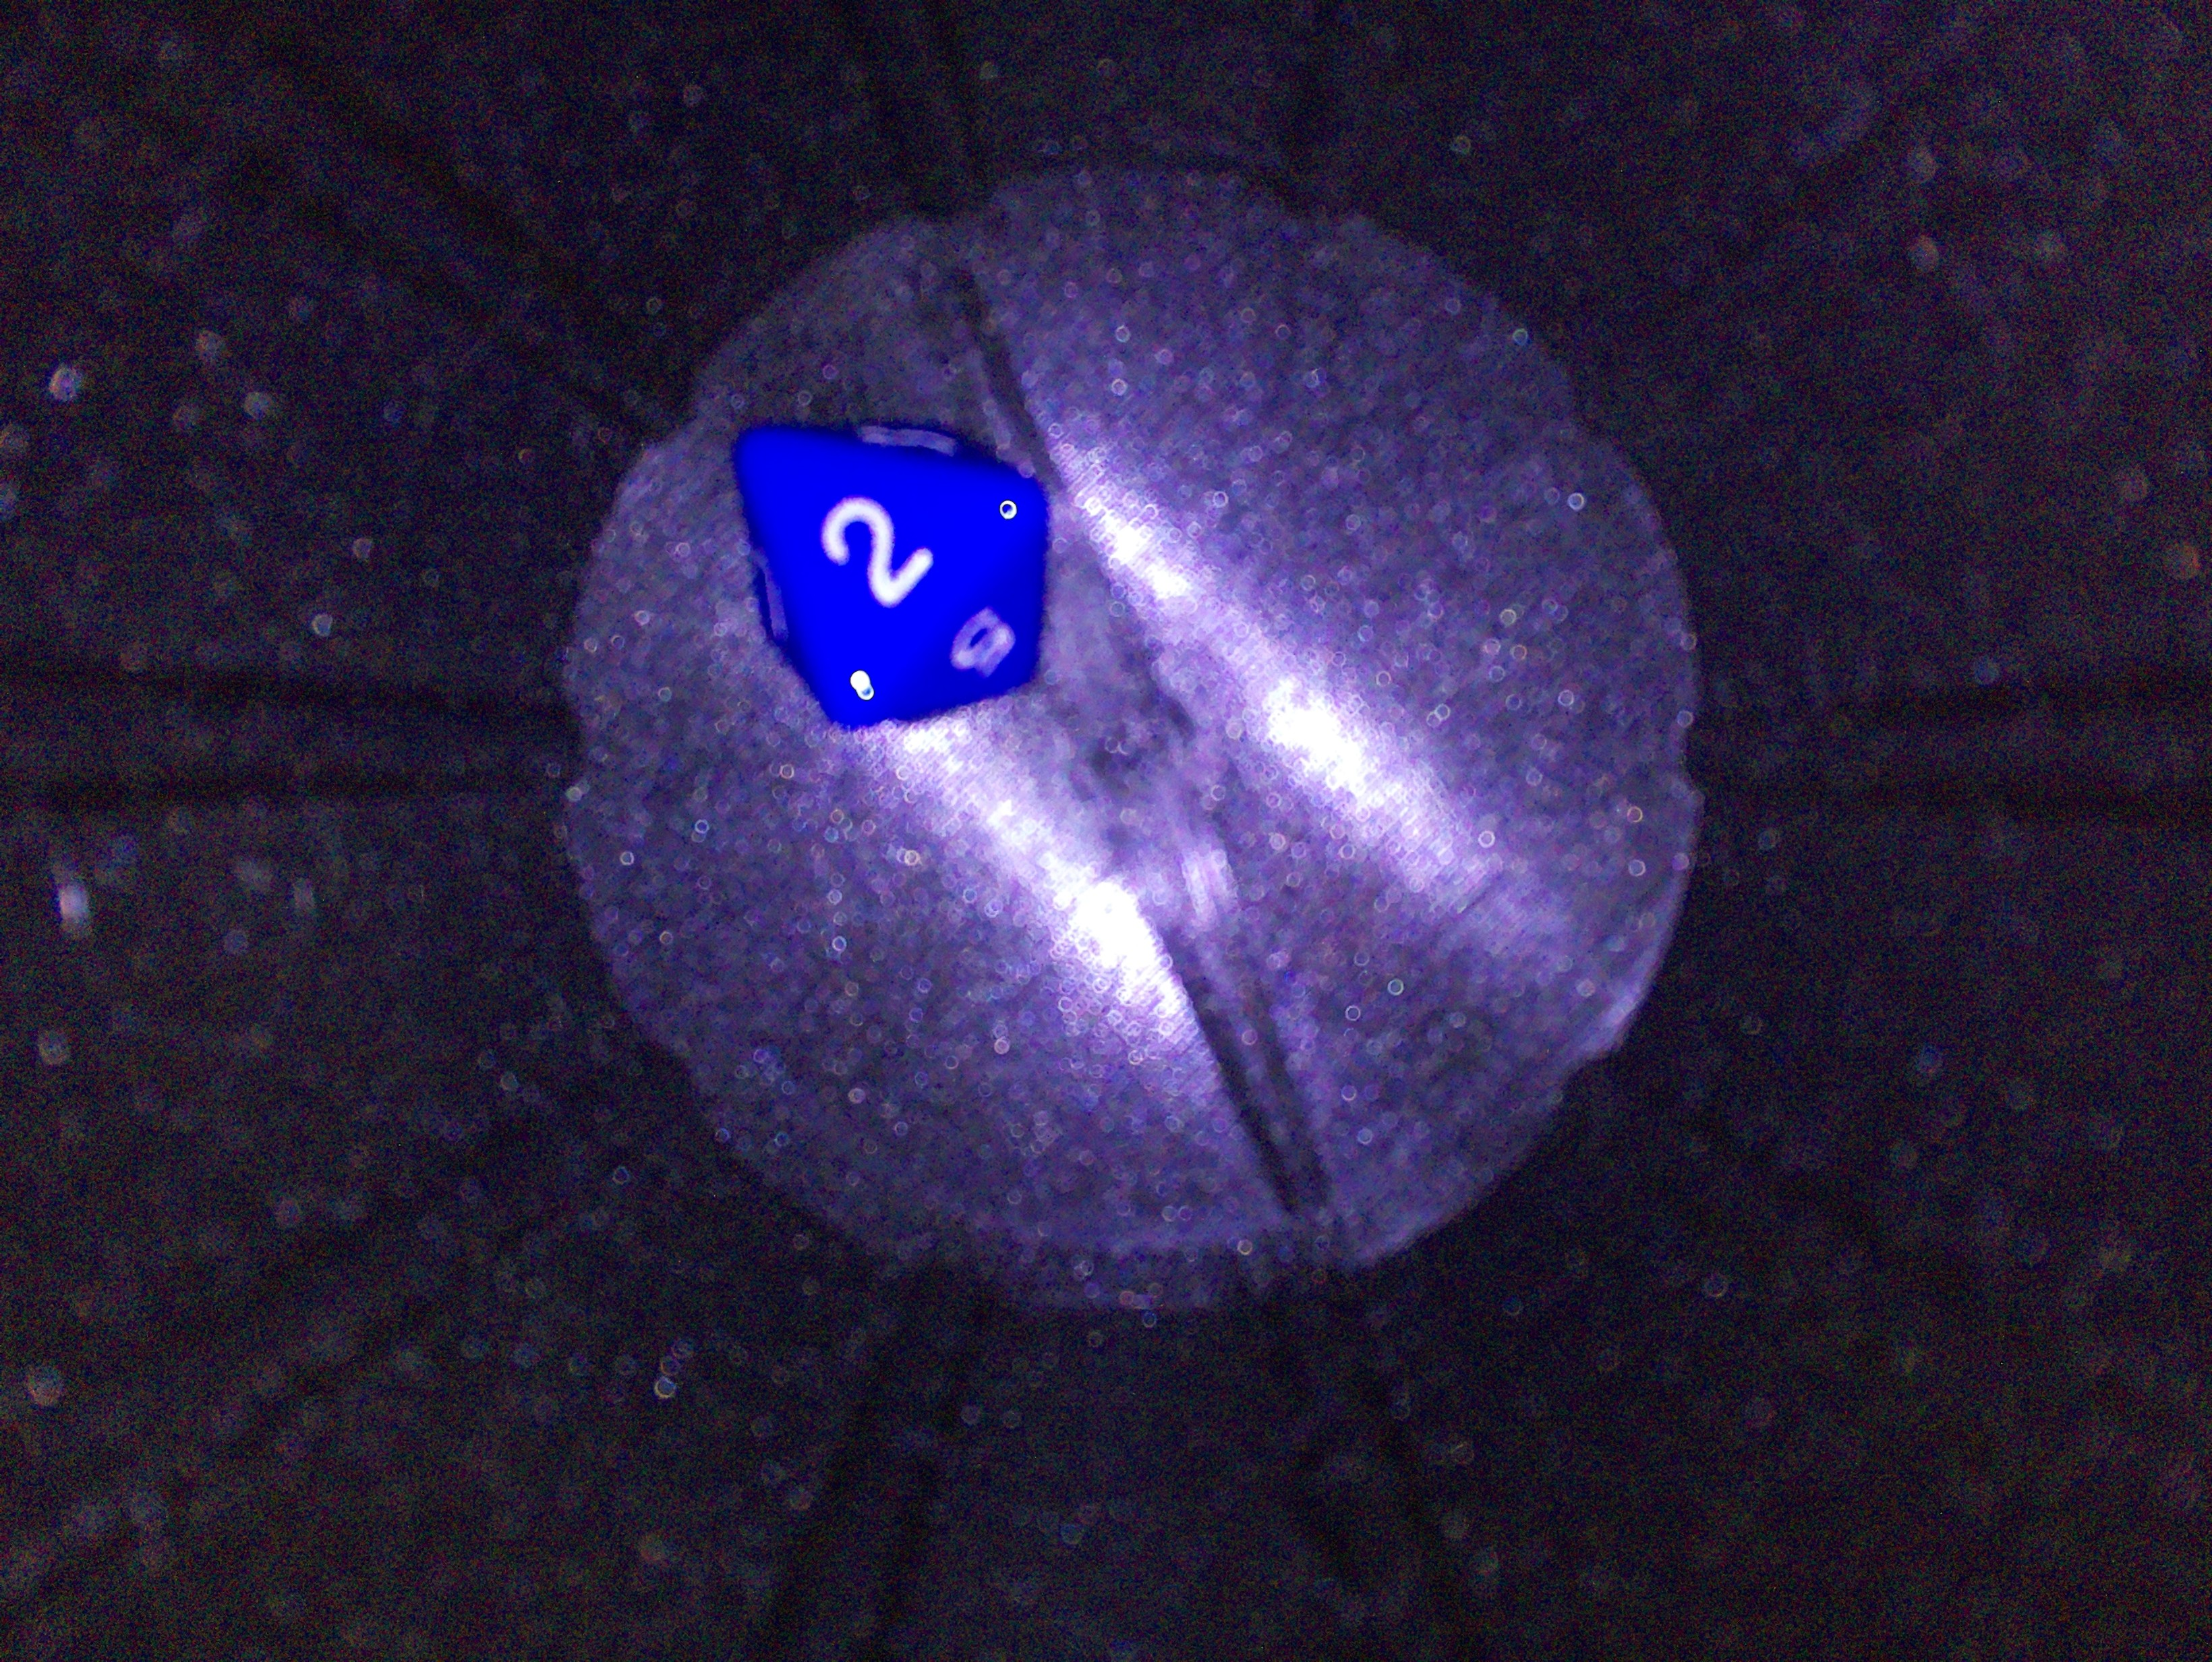
\includegraphics[height=4cm]{chapters/04-czytanie/figures/2_1}
        \caption{Etap 1: Surowe zdjęcie.}
        \label{fig:step1}
    \end{subfigure}
    \hspace{-0.5em}
    \begin{subfigure}[t]{0.32\linewidth}
        \centering
        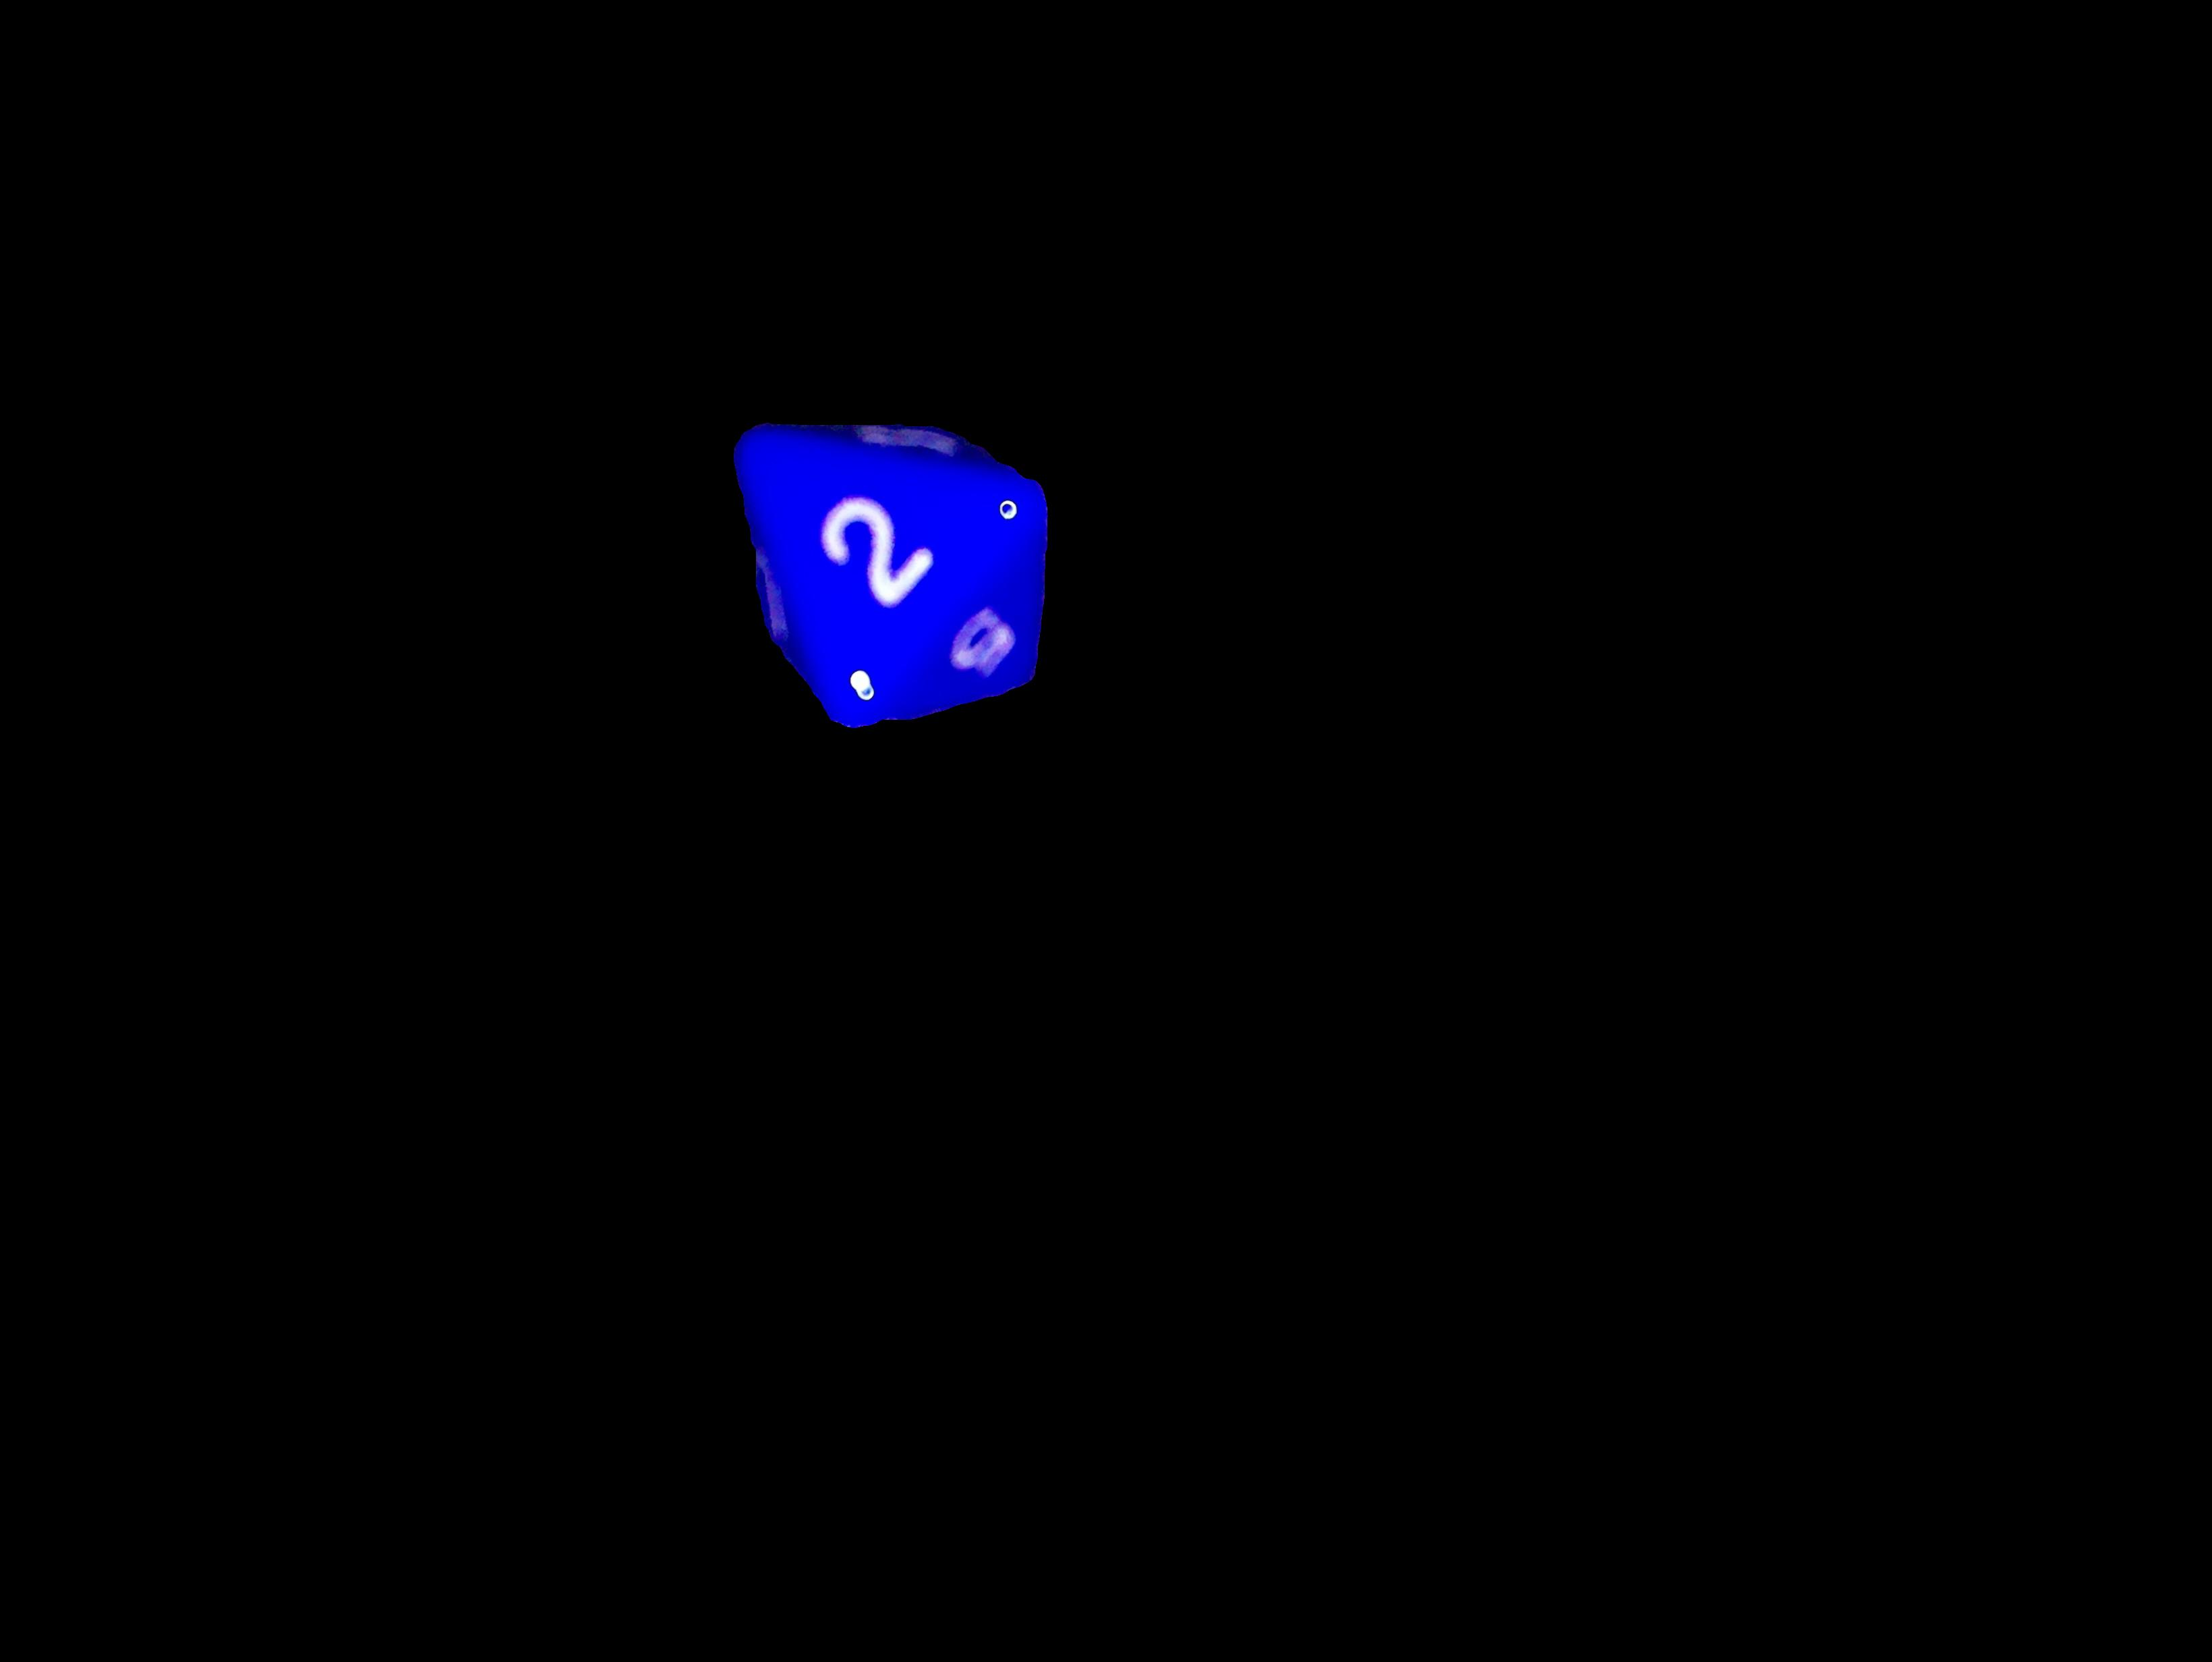
\includegraphics[height=4cm]{chapters/04-czytanie/figures/2_2}
        \caption{Etap 2: Nałożenie maski}
        \label{fig:step2}
    \end{subfigure}
    \hspace{-0.5em}
    \begin{subfigure}[t]{0.32\linewidth}
        \centering
        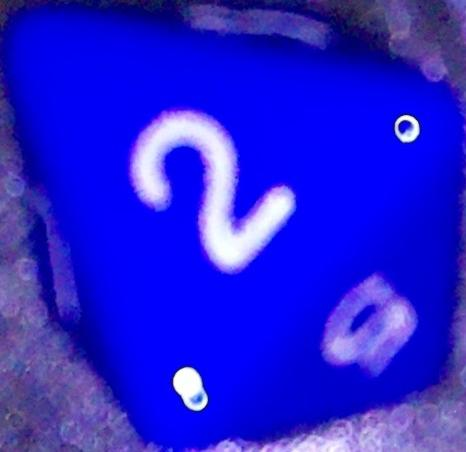
\includegraphics[height=4cm]{chapters/04-czytanie/figures/2_3}
        \caption{Etap 3: Wycięcie obszaru zainteresowania}
        \label{fig:step3}
    \end{subfigure}

    \vspace{0.3cm}

    \begin{subfigure}[t]{0.45\linewidth}
        \centering
        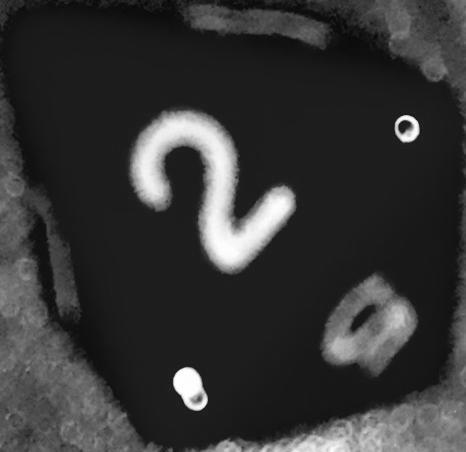
\includegraphics[height=4cm]{chapters/04-czytanie/figures/2_4}
        \caption{Etap 4: Skala szarości}
        \label{fig:step4}
    \end{subfigure}
    \hspace{0.5em}
    \begin{subfigure}[t]{0.45\linewidth}
        \centering
        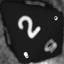
\includegraphics[height=4cm]{chapters/04-czytanie/figures/2_5}
        \caption{Etap 5: Wynik końcowy.}
        \label{fig:step5}
    \end{subfigure}

    \caption{Kolejne etapy przetwarzania obrazu. Wszystkie obrazy mają równą wysokość.}
    \label{fig:preproc_steps}
\end{figure}


Przedstawiony algorytm został zaimplementowany w języku Python, a jego zadaniem jest identyfikacja,
wycięcie i przeskalowanie obszarów zawierających obiekty zainteresowania na zdjęciach.

Zdjęcia w formacie JPEG są wczytywane za pomocą modułu Pillow~\cite{pillow_docs},
który umożliwia konwersję obrazów do przestrzeni barw RGB, zapewniając jednolitość formatów danych wejściowych.
Następnie obrazy są przekształcane do przestrzeni barw HSV,
co pozwala oddzielić komponenty odpowiadające za barwę (H), nasycenie (S) oraz jasność (V).

Komponent nasycenia (S) jest wygładzany za pomocą filtru Gaussa~\cite{gaussian_filter},
również dostępnego w ramach tego samego modułu,
co redukuje szumy i pozwala na bardziej precyzyjną analizę.
Wykorzystano parametry filtru z maską o wymiarach $5 \times 5$ pikseli oraz odchyleniem standardowym równym 1.
Takie ustawienia zapewniają balans między wygładzeniem a zachowaniem szczegółów obrazu.

Na podstawie wygładzonego komponentu nasycenia za pomocą progowania tworzona jest maska binarna,
która identyfikuje obszary o wysokim nasyceniu, odpowiadające obiektom zainteresowania (kości).
Próg został dobrany eksperymentalnie, kończąc na wartości 224,
tak aby w kontrolowanym środowisku (opisanym w poprzednim rozdziale) maska obejmowała obszar zainteresowania,
ale nie obejmowała tła (czarnego kubka).
Korzysta to z faktu, że kubek wykonany jest z materiału o niskim nasyceniu,
a używana kość ma jednolity, jasny kolor, a więc i wysokie nasycenie.

W celu usunięcia niewielkich luk w masce binarnej stosowana jest operacja zamknięcia morfologicznego~\cite{morphological_closure}.
Operacja ta ujednolica maskę, co jest szczególnie istotne w przypadku obiektów o niejednorodnej strukturze nasycenia,
gdzie maska mogłaby zawierać rozłączne fragmenty obiektu.

Po zastosowaniu zamknięcia morfologicznego maska jest analizowana w celu
zlokalizowania największego konturu obejmującego obszar zainteresowania.
W tym celu wykorzystano funkcje biblioteki OpenCV~\cite{opencv_docs},
które umożliwiają zarówno zastosowanie domknięcia morfologicznego, jak i wykrycie konturu i obliczenie otaczającego go prostokąta.
Rozmiar prostokąta jest dynamicznie dopasowywany do obszaru maski.
%Domknięcie morfologiczne i zamknięcie morfologiczne to dokładnie to samo.

Na tej podstawie oryginalny obraz jest kadrowany w kształt prostokąta wokół obszaru zainteresowania,
a następnie przeskalowywany do wymiarów $64 \times 64$ pikseli.
Ostatecznie obraz jest konwertowany do skali szarości, co zmniejsza wymiarowość danych
i pozwala sieci neuronowej skupić się na strukturze obrazu.
Konwersja do skali szarości dodatkowo minimalizuje negatywny wpływ odblasków,
powstających gdy kość odbija światło wprost do kamery, co poprawia niezawodność analizy.



\subsection{Zidentyfikowane trudności i ich rozwiązania}\label{subsec:zidentyfikowane-trudnosci-i-ich-rozwiazania}

Wspomniane wcześniej odblaski znacznie pogarszają skuteczność odczytywania wyniku z kości.
Jednak zastosowanie skali szarości pozwoliło w znacznym stopniu pozbyć się tego problemu,
uwidaczniając widoczną na kości cyfrę, co pokazują rys. 4.3 oraz 4.4.

Dzięki zastosowaniu skali szarości łatwiej jest oddzielić jasne punkty będące wynikiem odblasku diody o ściankę kości,
od nieco ciemniejszych, lecz wciąż jasnych punktów oznaczających cyfrę na kości.

\begin{figure}[H]
    \centering
    \begin{subfigure}[t]{0.45\linewidth}
        \centering
        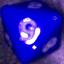
\includegraphics[width=\linewidth]{chapters/04-czytanie/figures/blask_raw}
        \caption{Odblask na przeskalowanym zdjęciu.}
        \label{fig:blaskraw}
    \end{subfigure}
    \hfill
    \begin{subfigure}[t]{0.45\linewidth}
        \centering
        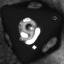
\includegraphics[width=\linewidth]{chapters/04-czytanie/figures/blask_proc}
        \caption{Odblask po zmianie na skalę szarości.}
        \label{fig:blaskproc}
    \end{subfigure}
    \caption{Porównanie odblasku przed i po przetworzeniu: część a) i b).}
    \label{fig:blaskcombined}
\end{figure}


Inną trudnością, która objawiała się w początkowych fazach pracy były zupełnie czarne obrazy,
w wyniku problemu z działaniem diod, jednak problem okazał się być spowodowany przez hardware, wynikający z awarii diody doświetlającej kubek.
Obecnie taki problem jest wykrywany oraz zgłaszany jest wyjątek oznaczający potrzebę naprawy usterki oświetlenia.
Nie był to jedyny problem powodowany przede wszystkim częścią sprzętową -- drugim takim było zatrzymanie śmigła w miejscu,
przez co do ewaluacji przez model kilkukrotnie trafiało identyczne, lub niemal identyczne zdjęcie.
To również zostało rozwiązane fizycznie, poprzez dodanie metalowej podkładki pod śmigłem,
ale mimo zażegnania problemu w taki sposób, zapewniono również obsługę wyjątku, który nadarzy się gdy wielokrotnie zostanie odczytana identyczna wartość.
W związku z ryzykiem fałszywego rozpoznania zatarcia śmigła przez losowo wypadającą wielokrotnie identyczną wartość ustawiono próg wykrywania takiej sytuacji i zgłaszania wyjątku na 13 identycznych odczytów z rzędu.
Statystyczna szansa na takie zdarzenie przy prawidłowej pracy maszyny wynosi
$\frac{1}{8^{12}} \approx 1{,}455 \times 10^{-11}$

Kolejną, znacznie częściej spotykaną trudnością w obecnej architekturze urządzenia są niejednoznaczne wyniki,
a więc moment, gdy kość zatrzyma się w pozycji, w której widać więcej niż jedną ściankę.
Najczęściej jest to spowodowane tym, że kość zatrzymała się na śmigle napędowym,
przez co wynik może być niejednoznaczny, co pokazano na rys.~\ref{fig:smiglocombined}.

\begin{figure}[h]
    \centering
    \begin{subfigure}[t]{0.45\linewidth}
        \centering
        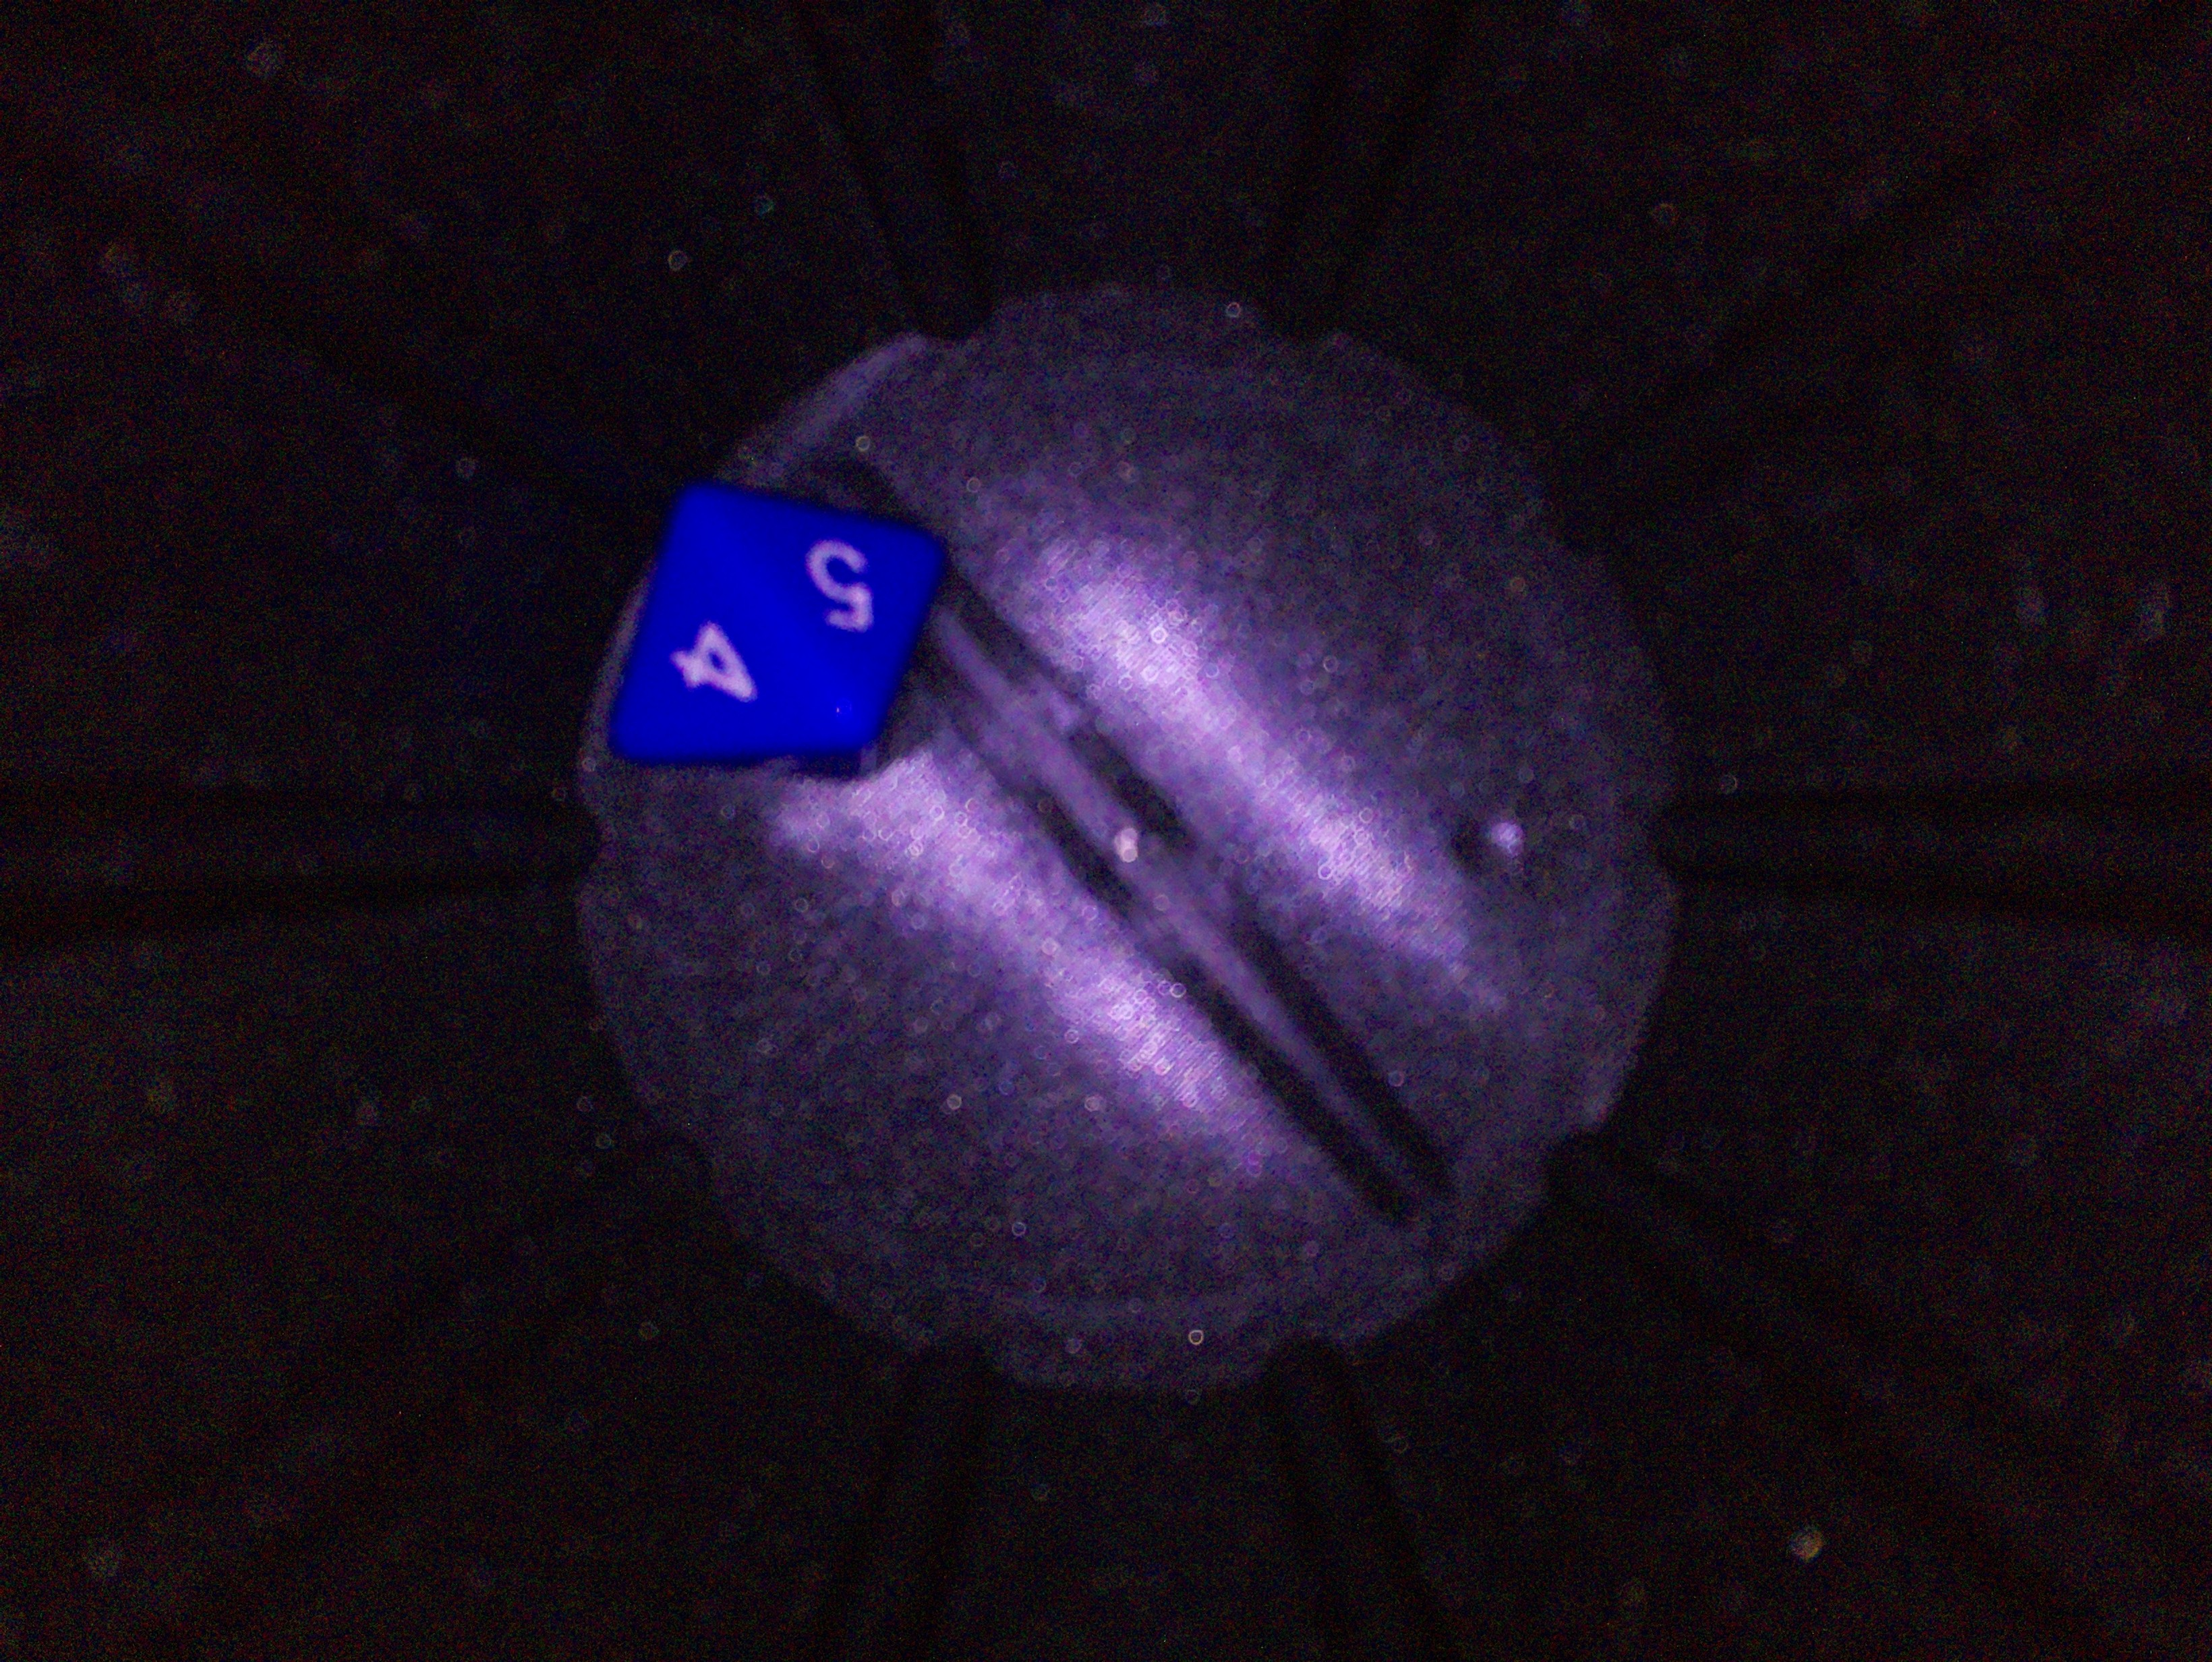
\includegraphics[width=\linewidth]{chapters/04-czytanie/figures/niepewne}
        \caption{Kość zatrzymana na śmigle (ujęcie 1).}
        \label{fig:niepewne}
    \end{subfigure}
    \hfill
    \begin{subfigure}[t]{0.45\linewidth}
        \centering
        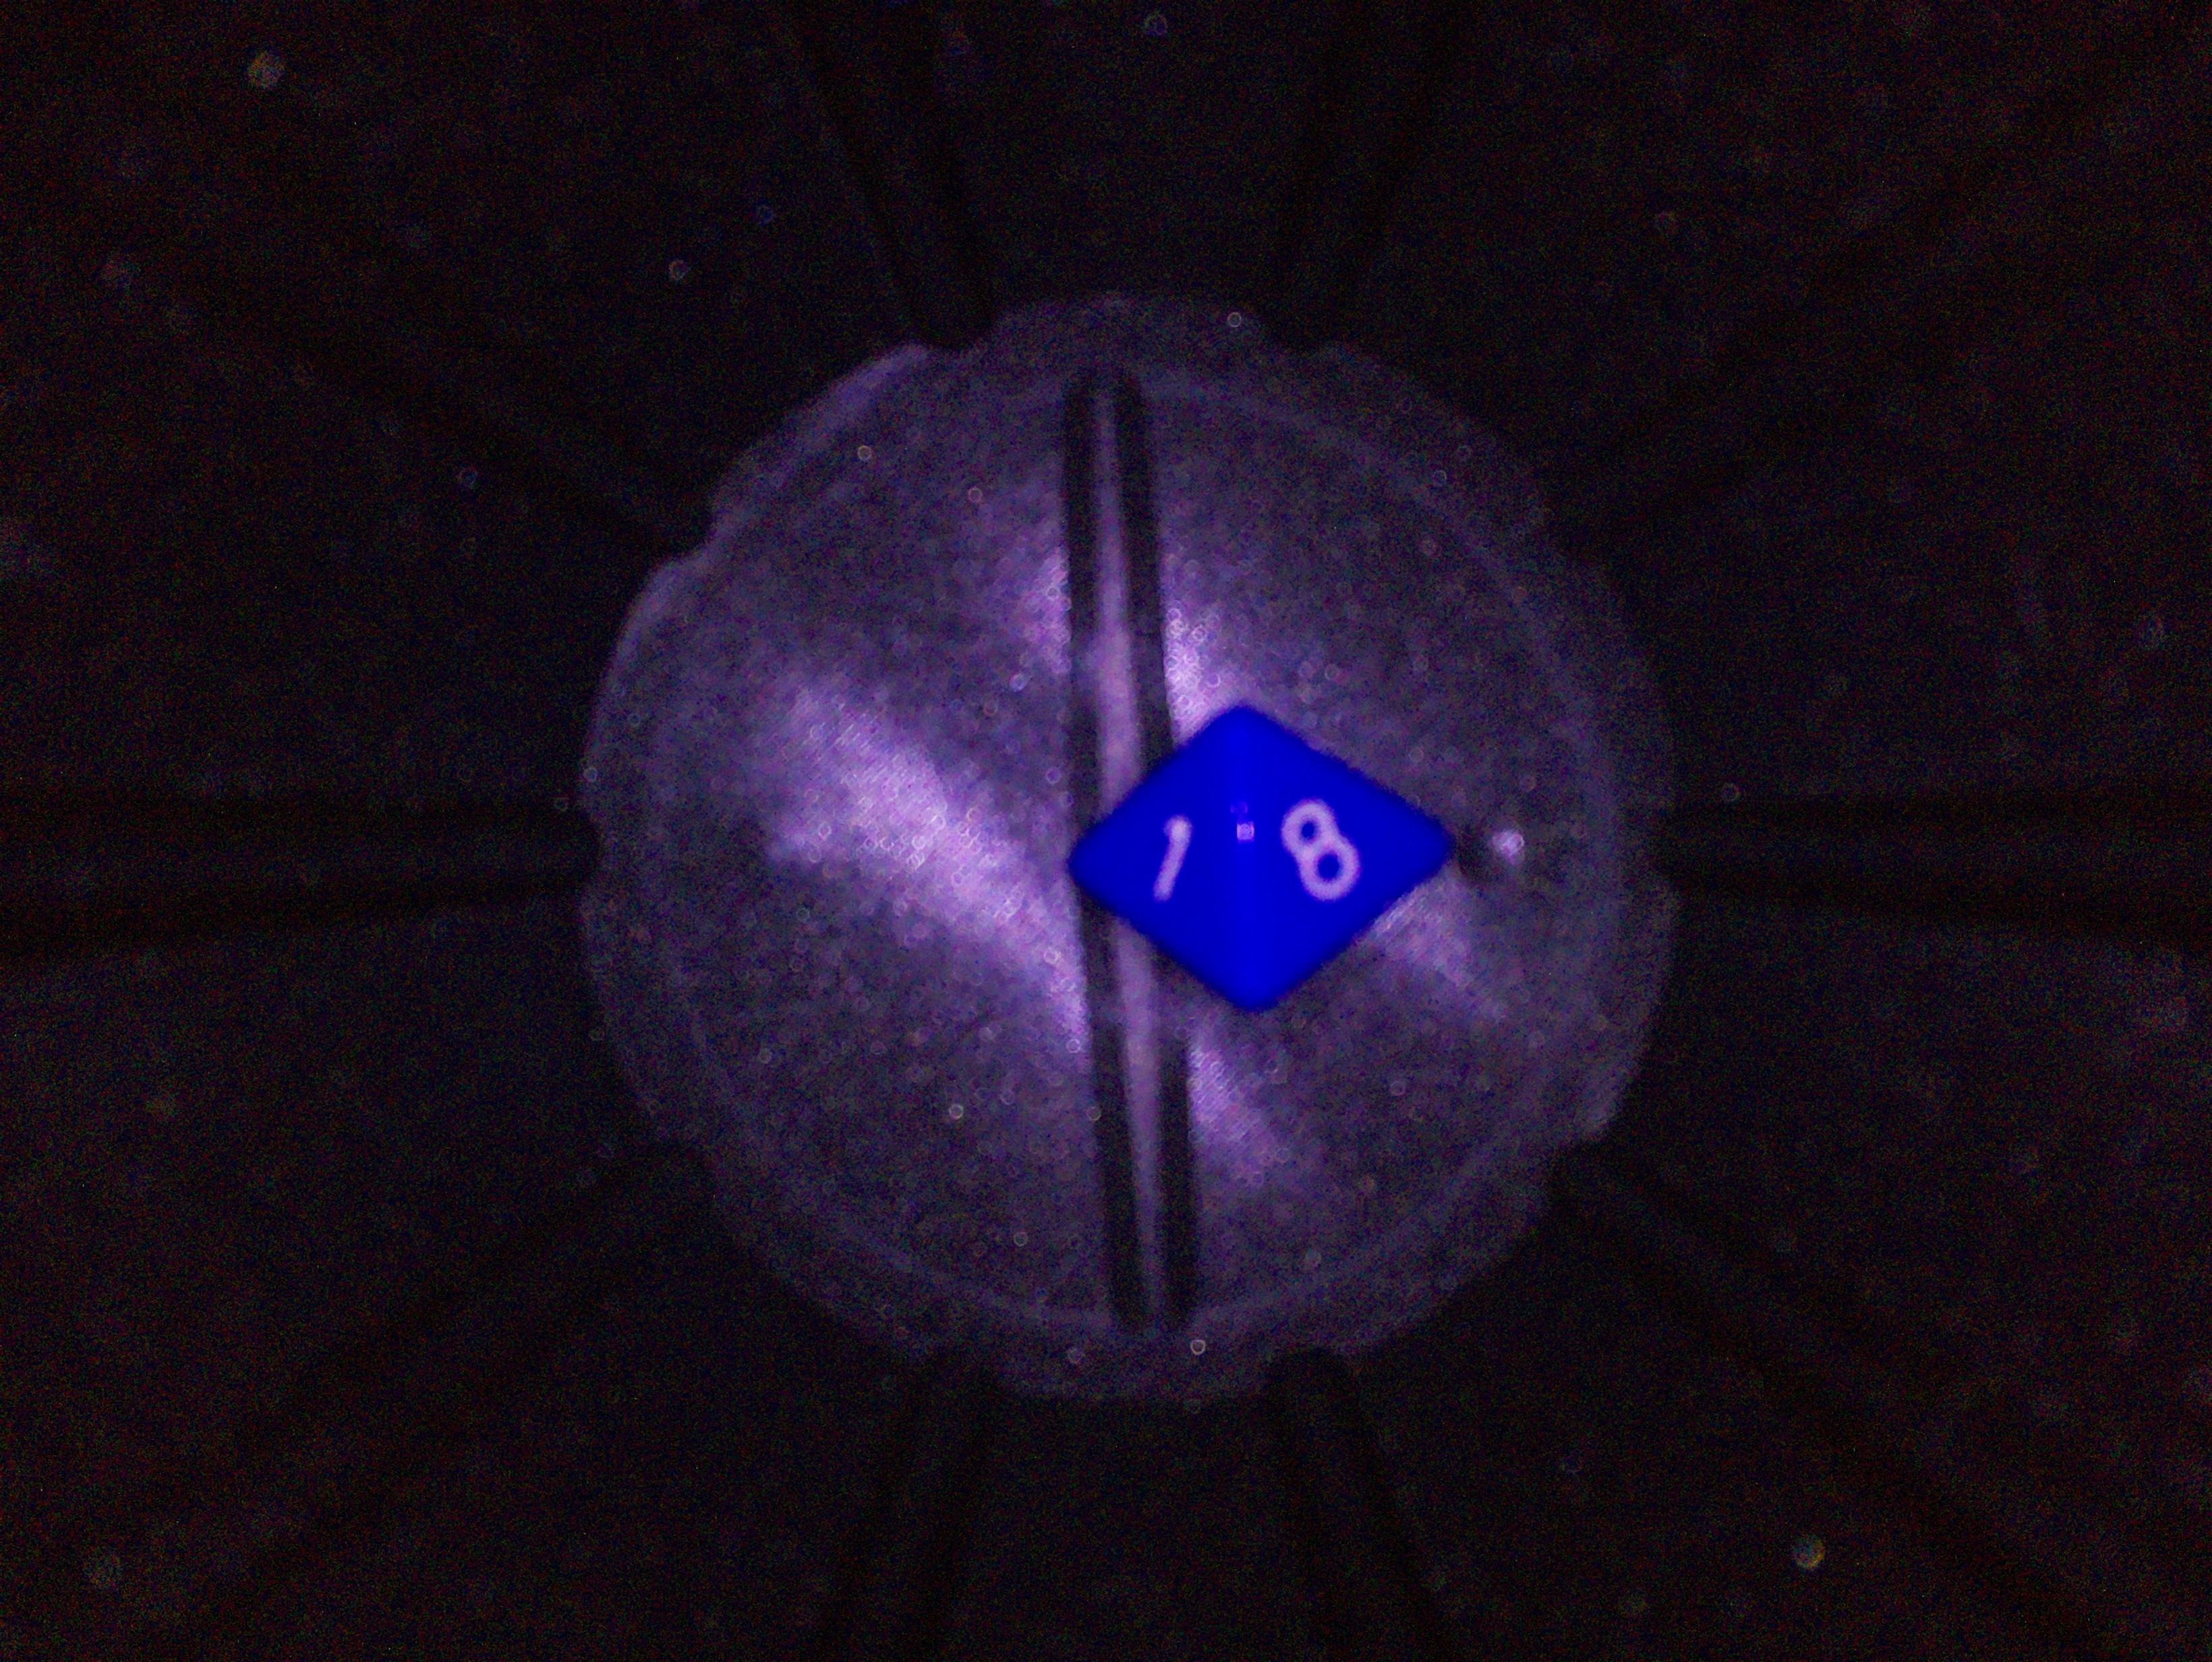
\includegraphics[width=\linewidth]{chapters/04-czytanie/figures/smiglo}
        \caption{Kość zatrzymana na śmigle (ujęcie 2).}
        \label{fig:smiglo}
    \end{subfigure}
    \caption{Porównanie dwóch ujęć kości zatrzymanej na śmigle.}
    \label{fig:smiglocombined}
\end{figure}


Rozwiązaniem tego problemu jest model dokonujący klasyfikacji wyniku rzutu, który odczytuje ze zdjęcia tylko jeden, najbardziej prawdopodobny wynik i wybiera ten,
który jest bardziej widoczny, ponieważ podczas uczenia model miał do czynienia z takimi niejednoznacznymi sytuacjami,
które zostały ręcznie oznaczone właśnie na potrzeby treningu modelu.

Zdarzają się również rzadkie przypadki, w których kość wyląduje równo na śmigle.
Jednakże w takim wypadku wynik jest idealnie czytelny,
identycznie jak gdy kość lądowała normalnie na podstawce kubka, więc nie jest to problemem.
%Wtedy problem z lądowaniem na śmigle nie istnieje,
%gdyż nie przeszkadza to w tym, że kość i tak zostanie podbita przy następnym obrocie śmigła.
Ostatnim rodzajem problemu, jaki został napotkany, był przypadek, w którym kość nie skończyła jeszcze swojej fazy lotu,
lub wpadła w bardzo długie wirowanie -- efektywnie uniemożliwiając odczytanie wyniku.
Przykłady zarejestrowanych przypadków wystąpienia tego problemu przestawiono na rys~\ref{fig:wircombined}.

\begin{figure}[h]
    \centering
    \begin{subfigure}[t]{0.45\linewidth}
        \centering
        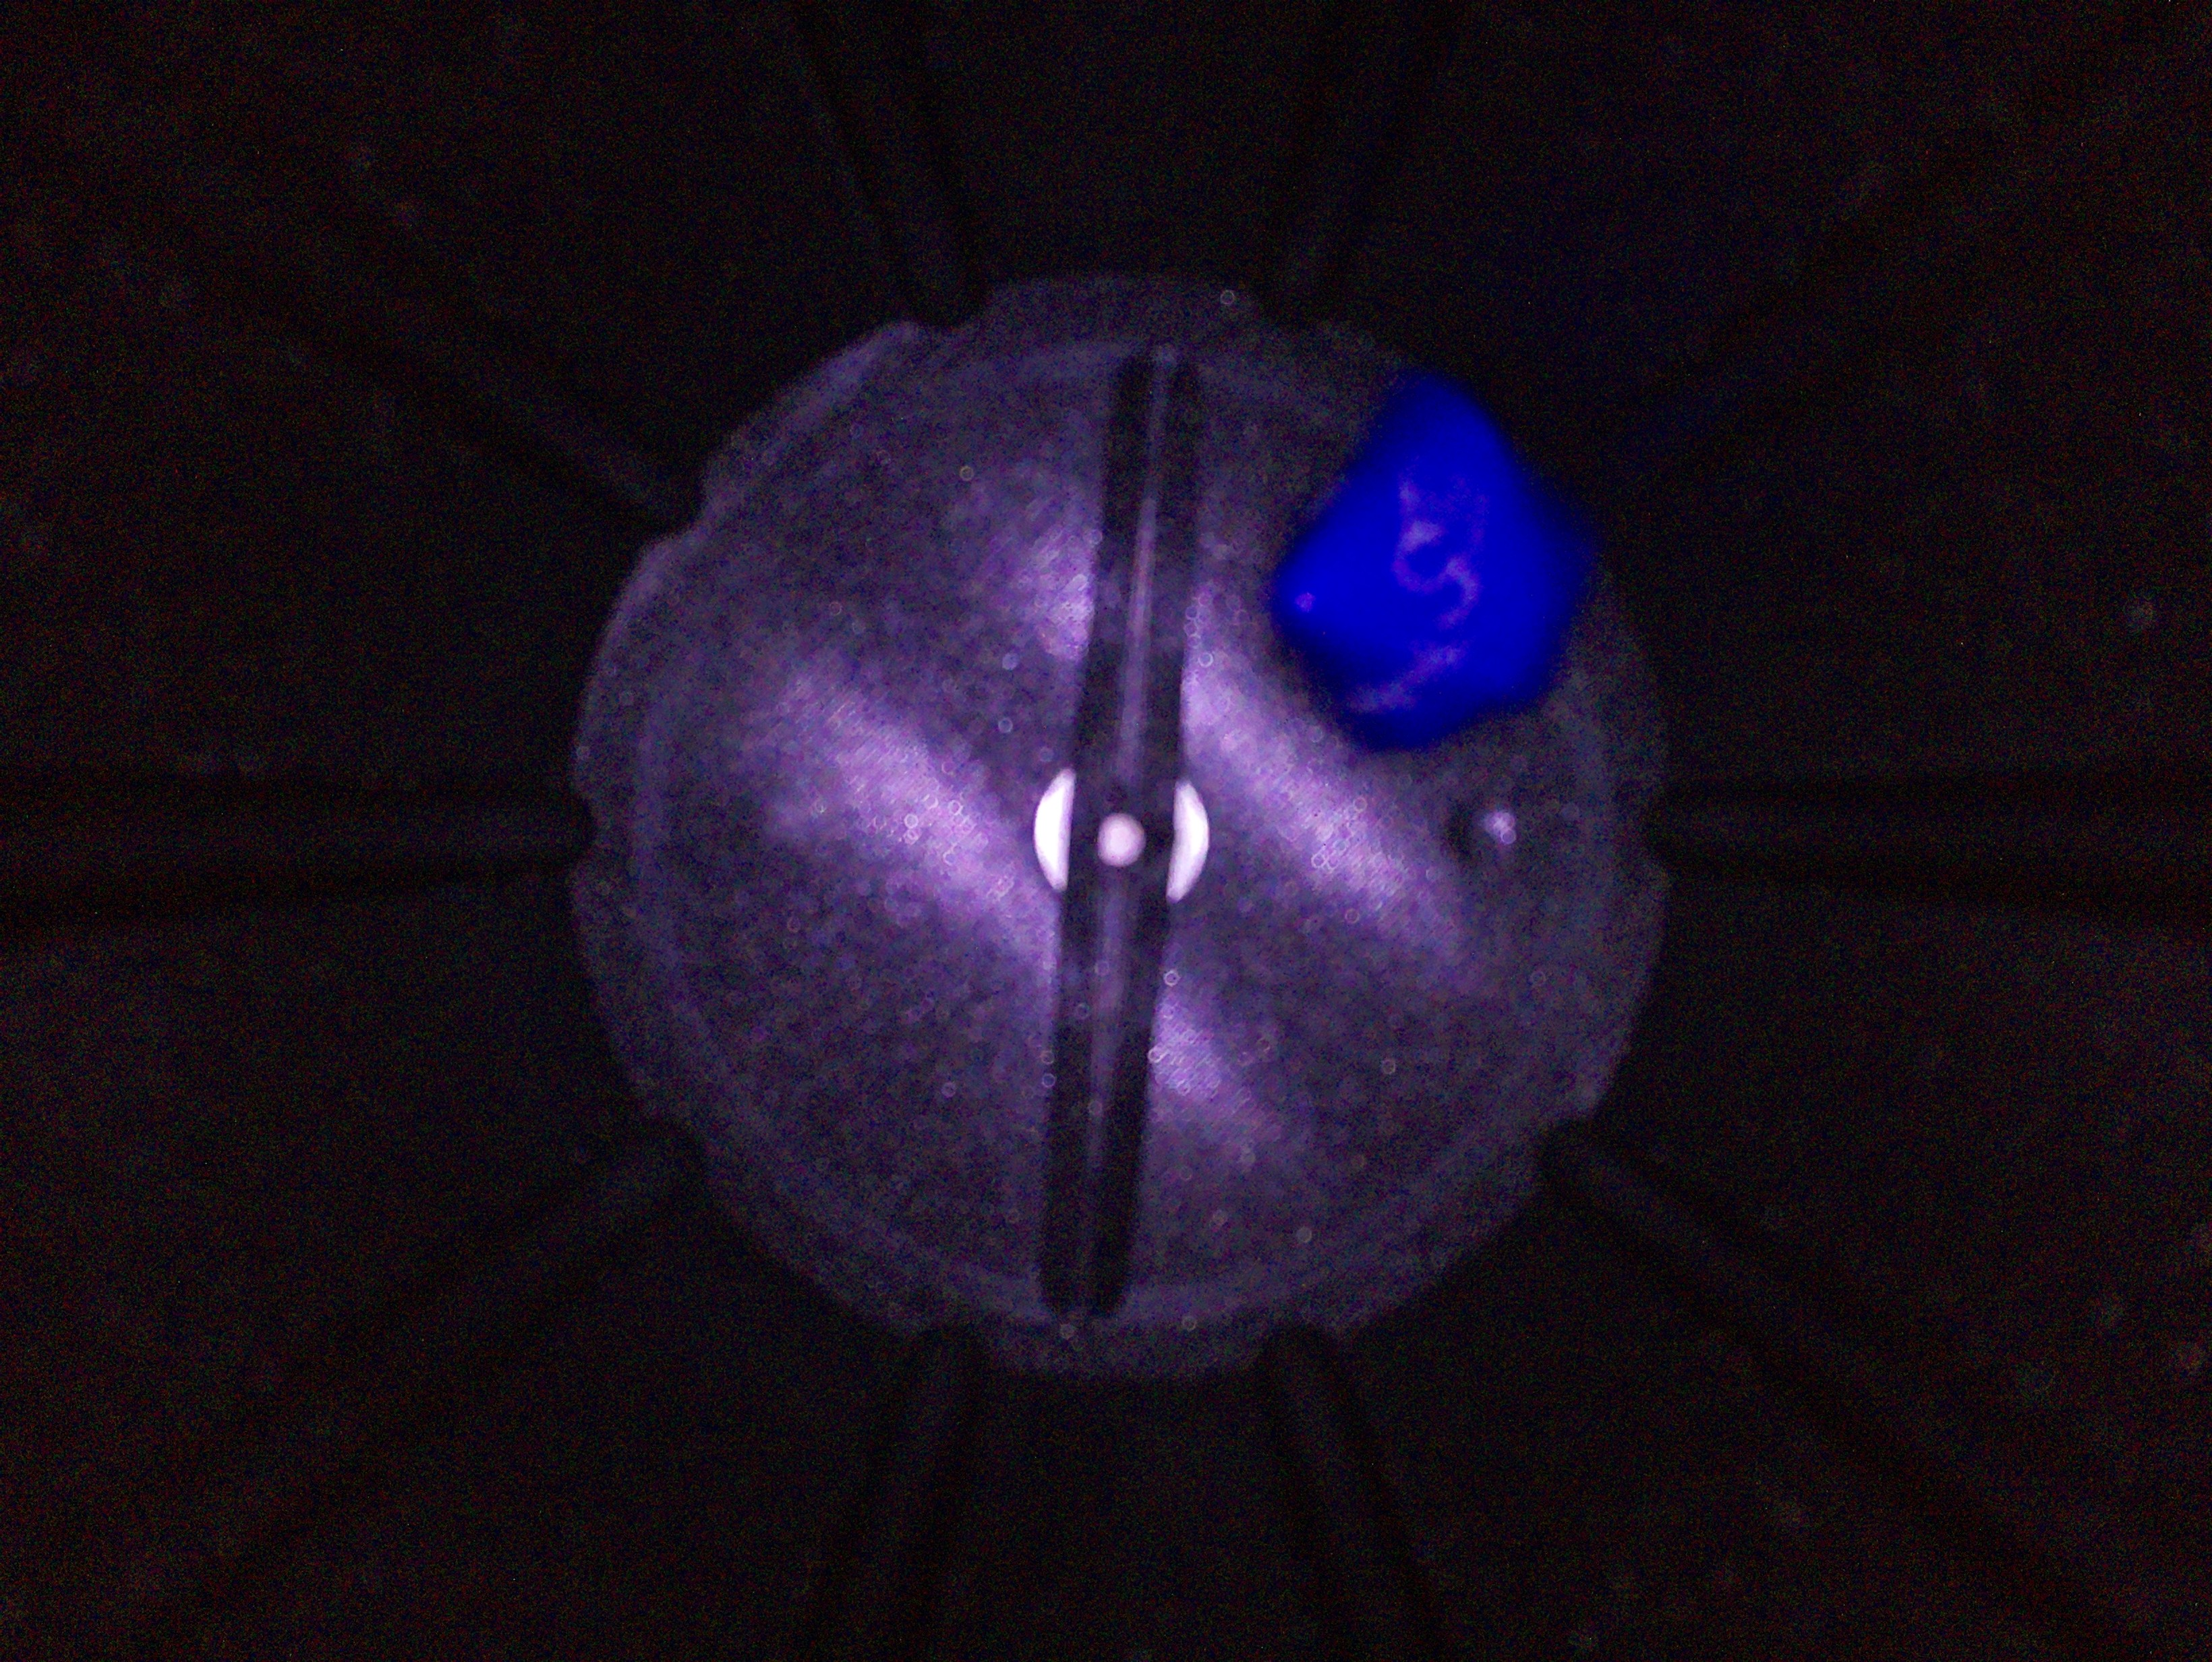
\includegraphics[width=\linewidth]{chapters/04-czytanie/figures/wir}
        \caption{Wirująca kość.}
        \label{fig:wir}
    \end{subfigure}
    \hfill
    \begin{subfigure}[t]{0.45\linewidth}
        \centering
        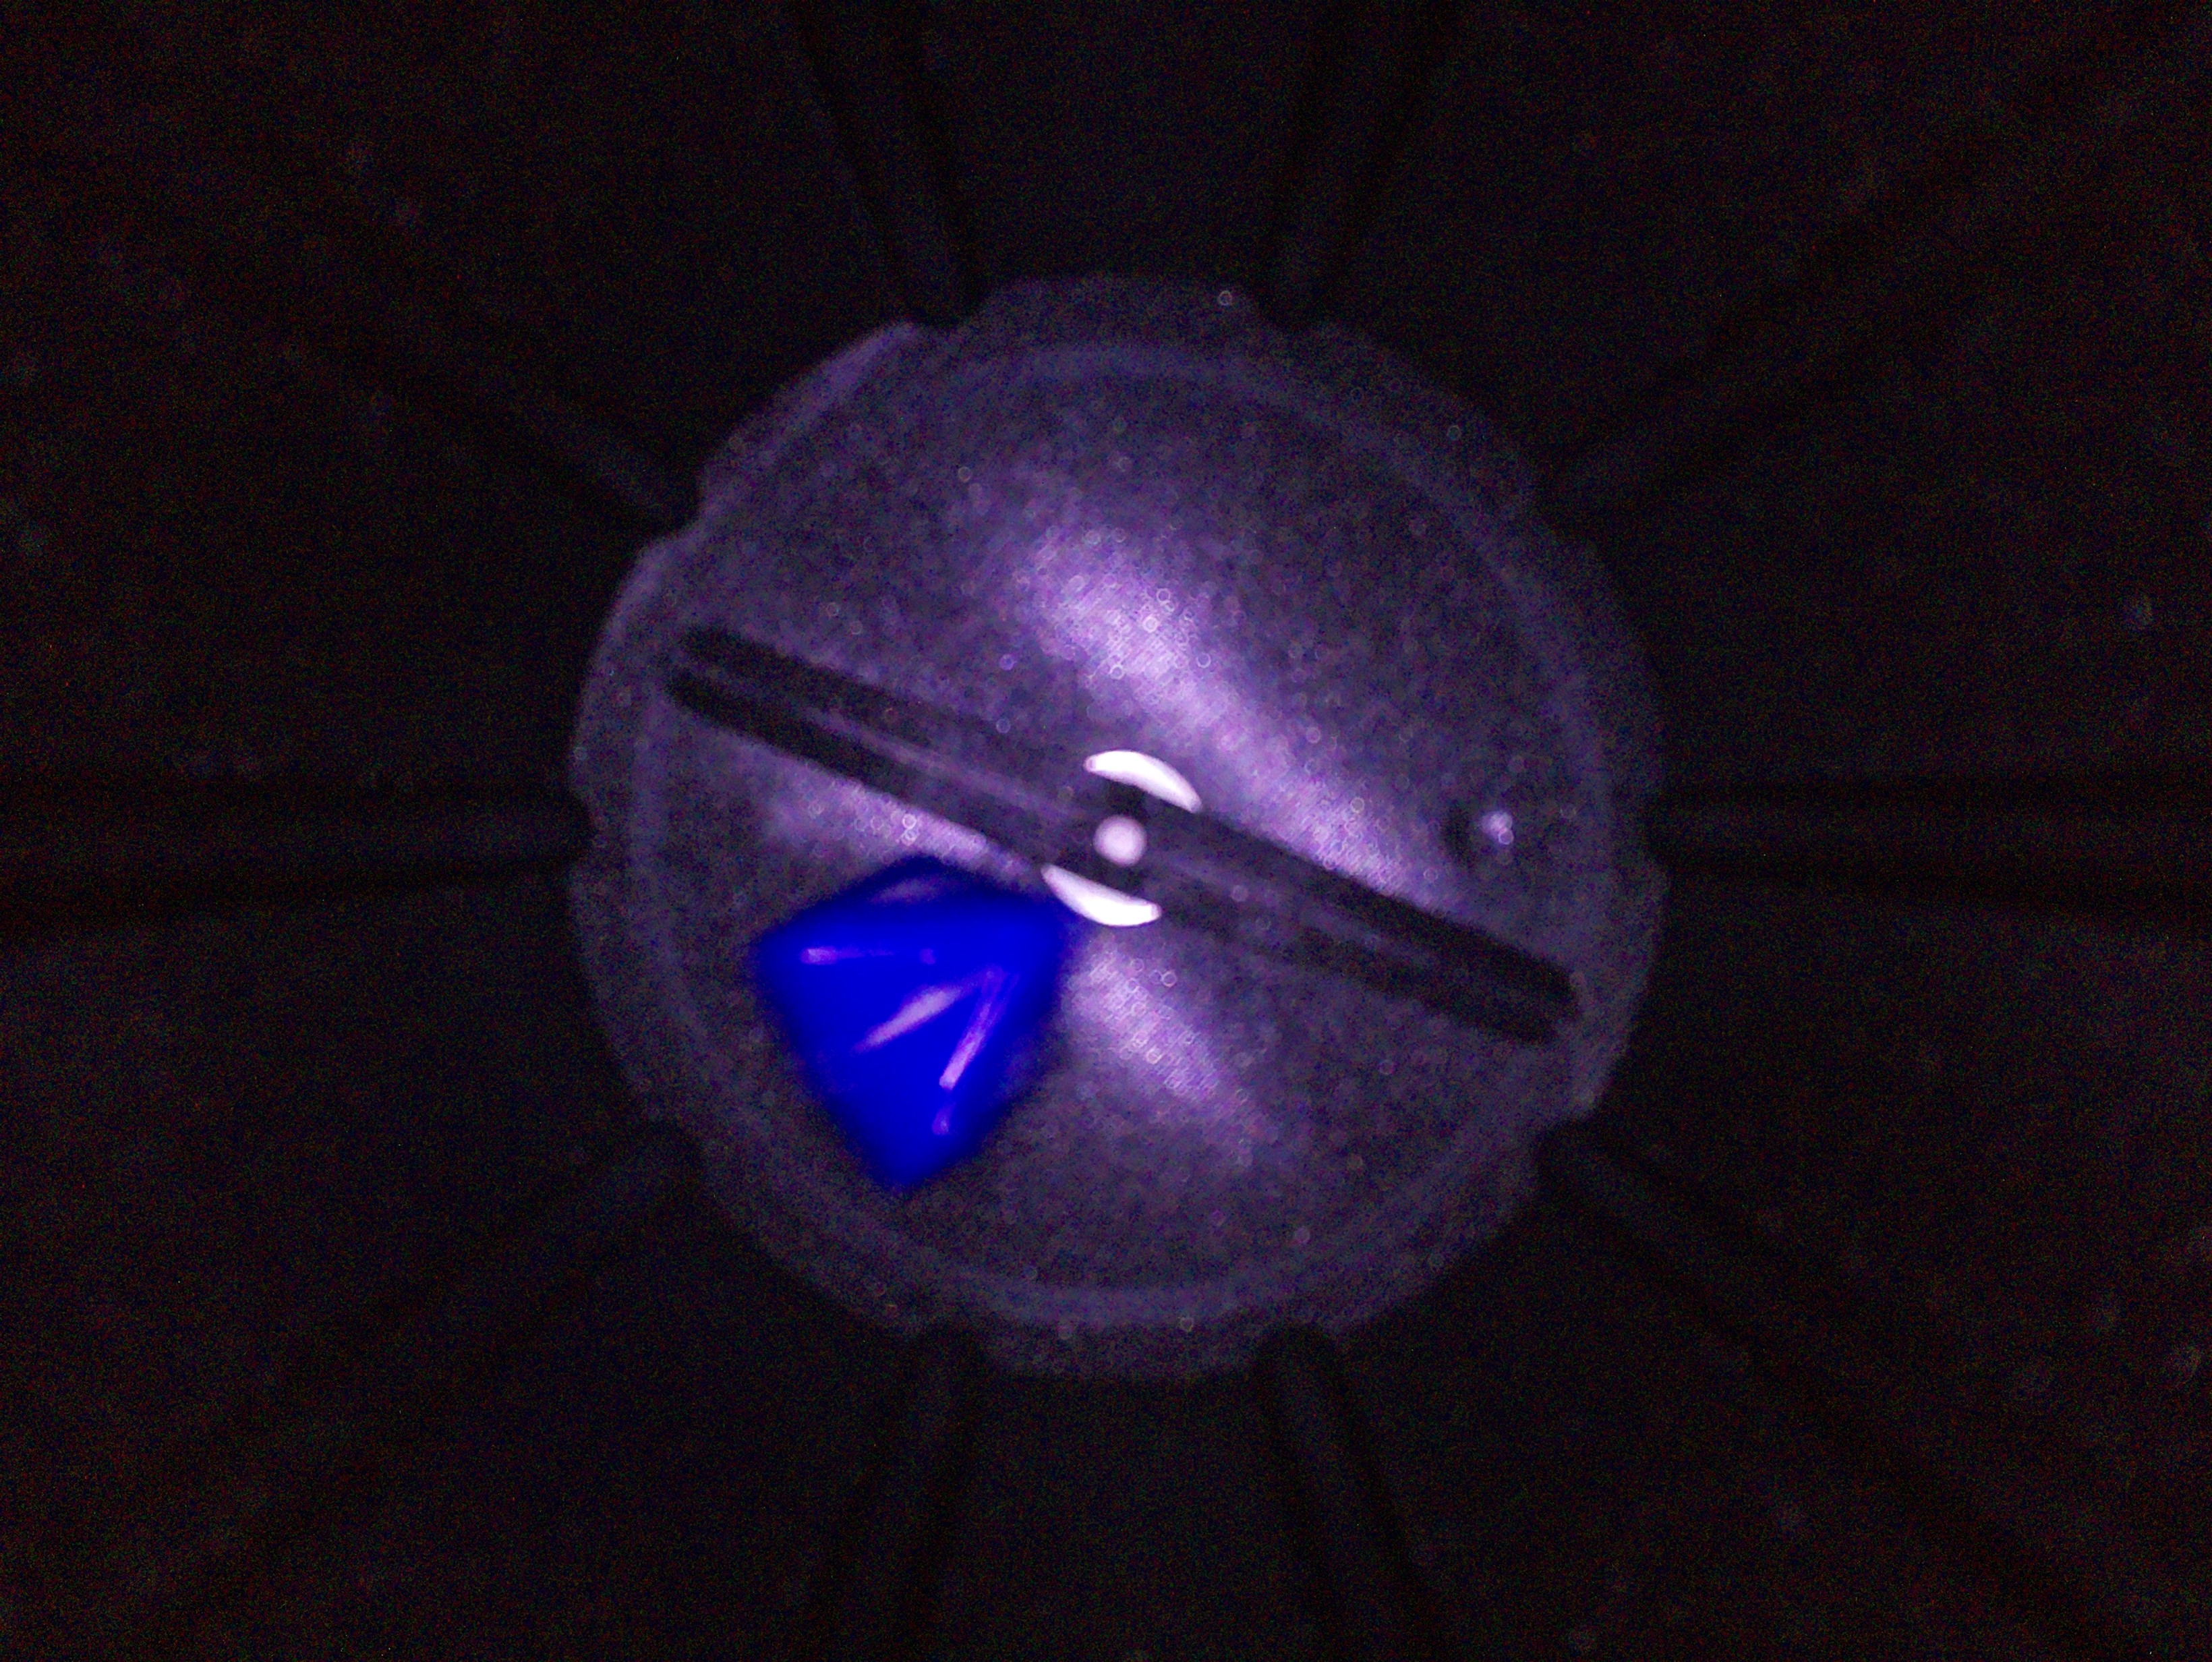
\includegraphics[width=\linewidth]{chapters/04-czytanie/figures/wir2}
        \caption{Kość w ruchu.}
        \label{fig:wir2}
    \end{subfigure}
    \caption{Nieczytelne ujęcia wynikające z dłuższego niż przewidywany ruchu kości}
    \label{fig:wircombined}
\end{figure}


Rozwiązaniem większości wypadków, w których zachodziła ta sytuacja, okazało się spowolnienie działania maszyny.
Obecnie oczekiwaniem aż kość zatrzyma się w miejscu steruje parametr czasowy, przyjmujący wartość jednej sekundy od zakończenia pracy śmigła.
Jest to wystarczające rozwiązanie, gdyż obecnie sytuacje niepewne z tego powodu zdarzają się bardzo rzadko (około 1 raz na 5000 rzutów).

Istnieje możliwość udoskonalenia tego rozwiązania, poprzez stosowanie detekcji ruchu kości,
jednak to rozwiązanie najpewniej okazałoby się bardziej kosztowne czasowo niż to proste czekanie stosowane obecnie.


\subsection{Podsumowanie}\label{subsec:podsumowanie}

Przedstawiony algorytm przetwarzania wstępnego pozwala na skuteczne przygotowanie danych wejściowych dla modelu sztucznej inteligencji.
Automatyzuje proces identyfikacji i kadrowania obiektów zainteresowania w obrazach, co znacząco poprawia jakość danych.
Rozwiązanie zostało zaprojektowane z myślą o łatwej adaptacji do innych zastosowań wymagających podobnego przetwarzania obrazów,
na przykład w przypadku zmiany kości w maszynie na inną, lub z inną liczbą ścianek.


\section{Opis Modelu SI}\label{sec:opis-modelu-si}

Model sztucznej inteligencji został zaprojektowany w celu klasyfikacji zdjęć kości ośmiościennych k8 do jednej z ośmiu klas,
odpowiadających cyfrom od 1 do 8 na każdej ze ścianek.
Do implementacji modelu wykorzystano przede wszystkim moduł TensorFlow~\cite{tensorflow_docs}
oraz wchodzący obecnie w jego skład Keras~\cite{keras_docs},
który umożliwia łatwe tworzenie i trenowanie sieci neuronowych.
%% uselesss :(( \textit{Biblioteka Keras jest wygodnym opakowaniem (wrapperem) dla modeli DL używanych do oszacowań klasyfikacji lub regresji]} [Donald J. Norris, 2020 s. 355 wydanie APN PROMISE SA]

\subsection{Przygotowanie danych}\label{subsec:przygotowanie-danych}

Dane wejściowe zostały podzielone na zestawy treningowy i walidacyjny w proporcji 70:30.
W celu zwiększenia różnorodności danych treningowych zastosowano techniki augmentacji obrazów dostępne w klasie
\texttt{ImageDataGenerator}~\cite{keras_imagedatagenerator}, takie jak:

\begin{itemize}
    \item obrót o losowy kąt w zakresie do 90°,
    \item przesunięcia poziome i pionowe w zakresie $\pm 20\%$ wymiarów obrazu,
    \item transformacje perspektywiczne (ang. \textit{shear}) w zakresie $\pm 10\%$,
    \item losowe przybliżenia lub oddalenia (ang. \textit{zoom}) w zakresie $90\%-110\%$ oryginalnego obrazu.
\end{itemize}

Wszystkie augmentacje przedstawiono na rys.~\ref{fig:5augment}
Dodatkowo, obrazy są normalizowane do zakresu $[0, 1]$, co pozwala na skuteczniejsze działanie sieci neuronowej.

\begin{figure}[h]
    \centering
    \begin{subfigure}[t]{0.32\linewidth}
        \centering
        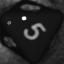
\includegraphics[width=\linewidth]{chapters/04-czytanie/figures/5_preprocessed}
        \caption{Obraz po preprocessingu, bazowy dla augmentacji.}
        \label{fig:5raw}
    \end{subfigure}
    \hfill
    \begin{subfigure}[t]{0.32\linewidth}
        \centering
        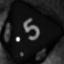
\includegraphics[width=\linewidth]{chapters/04-czytanie/figures/5_rotate}
        \caption{Obraz po obrocie.}
        \label{fig:5rotate}
    \end{subfigure}
    \hfill
    \begin{subfigure}[t]{0.32\linewidth}
        \centering
        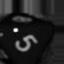
\includegraphics[width=\linewidth]{chapters/04-czytanie/figures/5_shift}
        \caption{Obraz po przesunięciu.}
        \label{fig:5move}
    \end{subfigure}

    \vspace{0.5cm} % Odstęp między wierszami obrazków

    \begin{subfigure}[t]{0.32\linewidth}
        \centering
        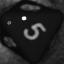
\includegraphics[width=\linewidth]{chapters/04-czytanie/figures/5_shear}
        \caption{Obraz po ścinaniu.}
        \label{fig:5shear}
    \end{subfigure}
    \hfill
    \begin{subfigure}[t]{0.32\linewidth}
        \centering
        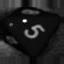
\includegraphics[width=\linewidth]{chapters/04-czytanie/figures/5_zoom}
        \caption{Obraz po powiększeniu.}
        \label{fig:5zoom}
    \end{subfigure}
    \hfill
    \begin{subfigure}[t]{0.32\linewidth}
        \centering
        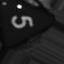
\includegraphics[width=\linewidth]{chapters/04-czytanie/figures/combined_1}
        \caption{Obraz wynikowy.}
        \label{fig:5combined}
    \end{subfigure}

    \caption{Różne składowe augmentacji obrazów uczących}
    \label{fig:5augment}
\end{figure}


W szczególności należy zaznaczyć, że finalnie uniknięto początkowo przeoczonego błędu,
jakim jest tworzenie obrazów lustrzanych w wyżej wymienionych transformacjach, gdyż obrazy lustrzane
sprawiały, że ścianki 2 oraz 5 były znacznie gorzej rozróżnialne przez wytrenowany model.
Problem nie był początkowo łatwy do wykrycia, gdyż zdjęcia odbite zarówno w pionowej jak i poziomej osi były poprawne,
a niepoprawne były te odbite tylko wobec jednej osi, czego przykład można zaobserwować na rys.~\ref{fig:25confusion}.


\begin{figure}[h]
    \centering
    \begin{subfigure}[t]{0.45\linewidth}
        \centering
        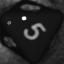
\includegraphics[width=\linewidth]{chapters/04-czytanie/figures/5_preprocessed}
        \caption{Zdjęcie przedstawiające 5}
        \label{fig:5_confusion}
    \end{subfigure}
    \hfill
    \begin{subfigure}[t]{0.45\linewidth}
        \centering
        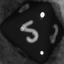
\includegraphics[width=\linewidth]{chapters/04-czytanie/figures/2_mirror}
        \caption{Zdjęcie przedstawiające 2, odbite lustrzanie}
        \label{fig:2_confusion}
    \end{subfigure}
    \caption{Wizualne przedstawienie problemu dot. odbicia lustrzanego}
    \label{fig:25confusion}
\end{figure}


\section{Funkcja predict}

W celu rozpoznawania liczb na zdjęciach przetworzonych przez model stworzono funkcję \texttt{predict\_number},
która przekształca obraz do odpowiedniego formatu i zwraca przewidywaną klasę.
Funkcja działa w następujących krokach:

\subsection{Wczytanie i przetworzenie obrazu}

W przypadku funkcji dokonującej predykcji na pliku, obraz należy najpierw wczytać. Krok ten jest pomijany gdy do funkcji zostanie przekazany jako parametr obraz wczytany wcześniej.
TODO (to jeszcze nie istnieje, ale będzie istnieć w finalnej części, gdzie przetwarzanie będzie bardziej ``potokowe'' niźli wstadowe jak teraz, jeśli tak to można określić)
Obraz wejściowy wczytywany jest w trybie skali szarości i zmieniany na rozmiar zgodny z wymaganiami modelu ($64 \times 64$ pikseli):

\begin{verbatim}
img = image.load_img(img_path, target_size=(64, 64), color_mode='grayscale')
img_array = image.img_to_array(img) / 255.0
img_array = np.expand_dims(img_array, axis=0)
\end{verbatim}

Obraz jest normalizowany do zakresu $[0, 1]$, co pozwala na skuteczniejsze działanie sieci neuronowej.

\subsection{Predykcja klasy}

Przygotowany obraz jest przekazywany do modelu w celu uzyskania wyników predykcji:

\begin{verbatim}
prediction = model.predict(img_array)
predicted_class = np.argmax(prediction, axis=1)
\end{verbatim}

Funkcja \texttt{np.argmax} zwraca indeks klasy o najwyższym prawdopodobieństwie.

\subsection{Interpretacja wyniku}

Na podstawie indeksu przewidywanej klasy wybierana jest odpowiadająca jej etykieta (od 1 do 8):

\begin{verbatim}
class_names = ['1', '2', '3', '4', '5', '6', '7', '8']
predicted_label = class_names[predicted_class[0]]
return predicted_label
\end{verbatim}

Wynik funkcji to etykieta odpowiadająca numerowi na kości, co umożliwia dalsze wykorzystanie tego wyniku w systemie rozpoznawania liczb.

\section{Przetwarzanie wyniku}

Finalnie, zaetykietowany wynik przetwarzany jest na ciąg trzech bitów, odpowiadających etykiecie klasy.
Wyjątkiem w tym przetwarzaniu jest etykieta 8, gdyż w zapisie binarnym zawierała by 4 bity,
zamiast oczekiwanych trzech, jednak biorąc 3 najmniej znaczące bity (000)
jesteśmy w stanie zapewnić unikatowe kodowanie każdemu wynikowi.
W ten sposób, klasy 1-7 generują bity będące ich dosłowną reprezentacją binarną,
a 8 jest równoznaczne wyrzuceniu zera na kostce.



%TODO - ten rozdział w większości należy już do Kuby(P), ale zacząłem go jeszcze ja. Chyba że uważacie że ten szczegół należy zawrzeć jeszcze przy modelu, lub wprost tam zaetykietować klasę 8 jako 0 i przekazywać już 0, zamiast tłumaczyć 8 na 0 w tym miejscu tutaj.


\chapter{Testy}

Coś tam coś tam, mamy dwa warianty robota to możemy je porównać.

Do oceny losowości otrzymanych rozwiązań użyto:
\begin{itemize}
    \item test chi-kwadrat,
    \item test pojedynczych bitów,
    \item test serii,
    \item test długiej serii,
    \item test pokerowy.
\end{itemize}
(// nww czy to poprawne, po prostu przepisałam z kryptografii xD)

\section{Testy poszczególnych wariantów}
\subsection{Wariant 1 - \glqq Betoniarka\grqq}
\subsection{Wariant 2 - \glqq Blender\grqq}



\chapter{Zakończenie}

Zakończenie pracy
Lorem Ipsum Dolor sit itd. itp.


%--------------------------------------
% Literatura
%--------------------------------------

\bibliographystyle{plain}{\raggedright\sloppy\small\bibliography{bibliografia}}

%--------------------------------------
% Dodatki
%--------------------------------------

\cleardoublepage\appendix%
\newpage
% 
\chapter{Składanie dokumentu w systemie \LaTeX}

W tym rozdziale znajduje się
garść informacji o tym, jak poprawnie składać tekst pracy w systemie \LaTeX{} wraz z 
przykładami, które mają służyć do przeklejania do własnych dokumentów.

\section{Struktura dokumentu}
\chaptermark{Tytuł rozdziału, jeśli pełen się nie mieści\ldots{}}{}

Praca składa się z rozdziałów (\texttt{chapter}) i podrozdziałów (\texttt{section}).
Ewentualnie można również rozdziały zagnieżdzać (\texttt{subsection}, \texttt{subsubsection}),
jednak nie powinno się wykraczać poza drugi poziom hierarchii (czyli \texttt{subsubsection}).

\section{Akapity i znaki specjalne}

Akapity rozdziela się od siebie przynajmniej jedną pustą linią. Podstawowe
instrukcje, które się przydają to \emph{wyróżnienie pewnych słów}. Można również
stosować \textbf{styl pogrubiony}, choć nie jest to generalnie zalecane.

Należy pamiętać o zasadach polskiej interpunkcji i ortografii. Po spójnikach 
jednoliterowych warto wstawić znak tyldy ($\sim$), który jest tak zwaną
,,twardą spacją'' i powoduje, że wyrazy nią połączone nie będą rozdzielane
na dwie linie tekstu.

Polskie znaki interpunkcyjne różnią się nieco od angielskich: to jest ,,polski'', a to jest
``angielski''. W kodzie źródłowym tego tekstu będzie widać różnicę.

Proszę również zwrócić uwagę na znak myślnika, który może być pauzą ,,---'' lub
półpauzą: ,,--''. Należy stosować je konsekwentnie. Do łączenia wyrazów używamy
zwykłego ,,-'' (\emph{północno-wschodni}), do myślników --- pauzy lub półpauzy.
Inne zasady interpunkcji i typografii można znaleźć w słownikach.

\section{Wypunktowania}

Wypunktowanie z cyframi:
\begin{enumerate}
    \item to jest punkt,
    \item i to jest punkt,
    \item a to jest ostatni punkt.
\end{enumerate}

\noindent
Po wypunktowaniach czasem nie warto wstawiać wcięcia akapitowego. Wtedy przydatne jest
polecenie \texttt{noindent}. Wypunktowanie z kropkami (tzw.~\emph{bullet list}) wygląda tak:
\begin{itemize}
    \item to jest punkt,
    \item i to jest punkt,
    \item a to jest ostatni punkt.
\end{itemize}

\noindent
Wypunktowania opisowe właściwie niewiele się różnią:
\begin{description}
    \item[elementA] to jest opis,
    \item[elementB] i to jest opis,
    \item[elementC] a to jest ostatni opis.
\end{description}


\section{Polecenia pakietu \texttt{ppfcmthesis}}

Parę poleceń zostało zdefiniowanych aby uspójnić styl pracy. Są one przedstawione poniżej
(oczywiście nie trzeba się do nich stosować).

\paragraph{Makra zdefiniowane dla języka angielskiego.} Są nimi: \texttt{termdef} oraz \texttt{acronym}.
Przykłady poniżej obrazują ich przewidywane użycie w tekście.
\begin{center}\footnotesize%
\begin{tabular}{l >{\rightskip\fill}p{12cm}}
\toprule
źródło   & \texttt{we call this a $\backslash$termdef\{Database Management System\} ($\backslash$acronym\{DBMS\})} \\ \cmidrule(lr){2-2}
docelowo & we call this a \termdef{Database Management System} (\acronym{DBMS}) \\ 
\bottomrule
\end{tabular}
\end{center}

\paragraph{Makra zdefiniowane dla języka polskiego.} Podobnie jak dla języka angielskiego zdefiniowano
odpowiedniki polskie: \texttt{defini\-cja}, \texttt{akronim} oraz \texttt{english} dla tłumaczeń angielskich
terminów. Przykłady poniżej obrazują ich przewidywane użycie w tekście.
\begin{center}\footnotesize%
\begin{tabular}{l >{\rightskip\fill}p{12cm}}
\toprule
źródło   & \texttt{nazywamy go $\backslash$definicja\{systemem zarządzania bazą danych\} ($\backslash$akronim\{DBMS\}, $\backslash$english\{Database Management System\})} \\ \cmidrule(lr){2-2}
docelowo & nazywamy go \definicja{systemem zarządzania bazą danych} (\akronim{DBMS}, \english{Database Management System}) \\ \bottomrule
\end{tabular}
\end{center}


\section{Rysunki}

Wszystkie rysunki (w tym również diagramy, szkice i inne) osadzamy w środowisku 
\texttt{figure} i umieszczamy podpis \emph{pod} rysunkiem, w formie elementu \texttt{caption}. Rysunki powinny
zostać umieszczone u góry strony (osadzone bezpośrednio w treści strony zwykle utrudniają czytanie tekstu).
Rysunek~\ref{rys:plama} zawiera przykład pełnego osadzenia rysunku na stronie.

\begin{figure}[t] % możliwe opcje to 't' - top, 'b' - bottom, 'h' - 'here', ale zaleca się 't'
\centering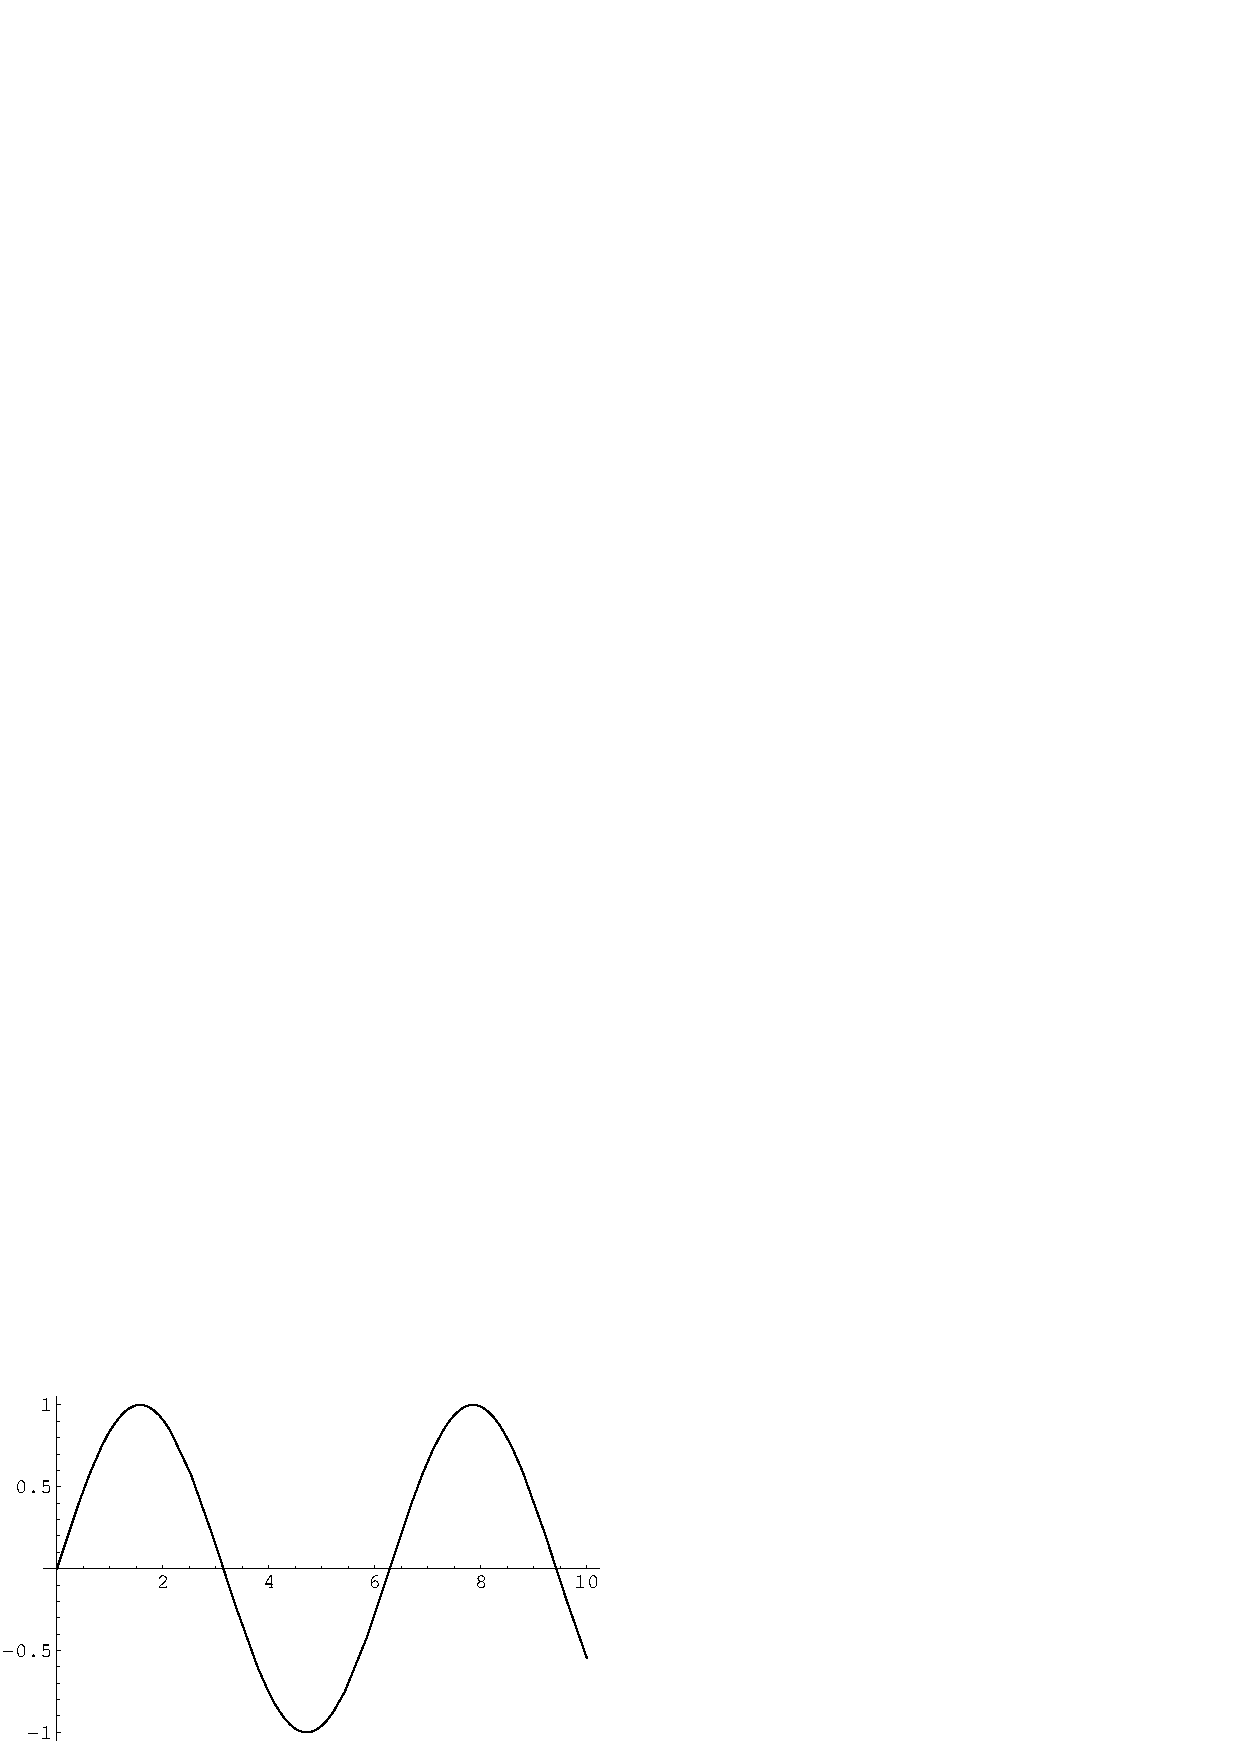
\includegraphics[width=5cm]{figures/mathematica}
\caption{Wykres.}\label{rys:plama}
\end{figure}

\begin{figure}[t]
\centering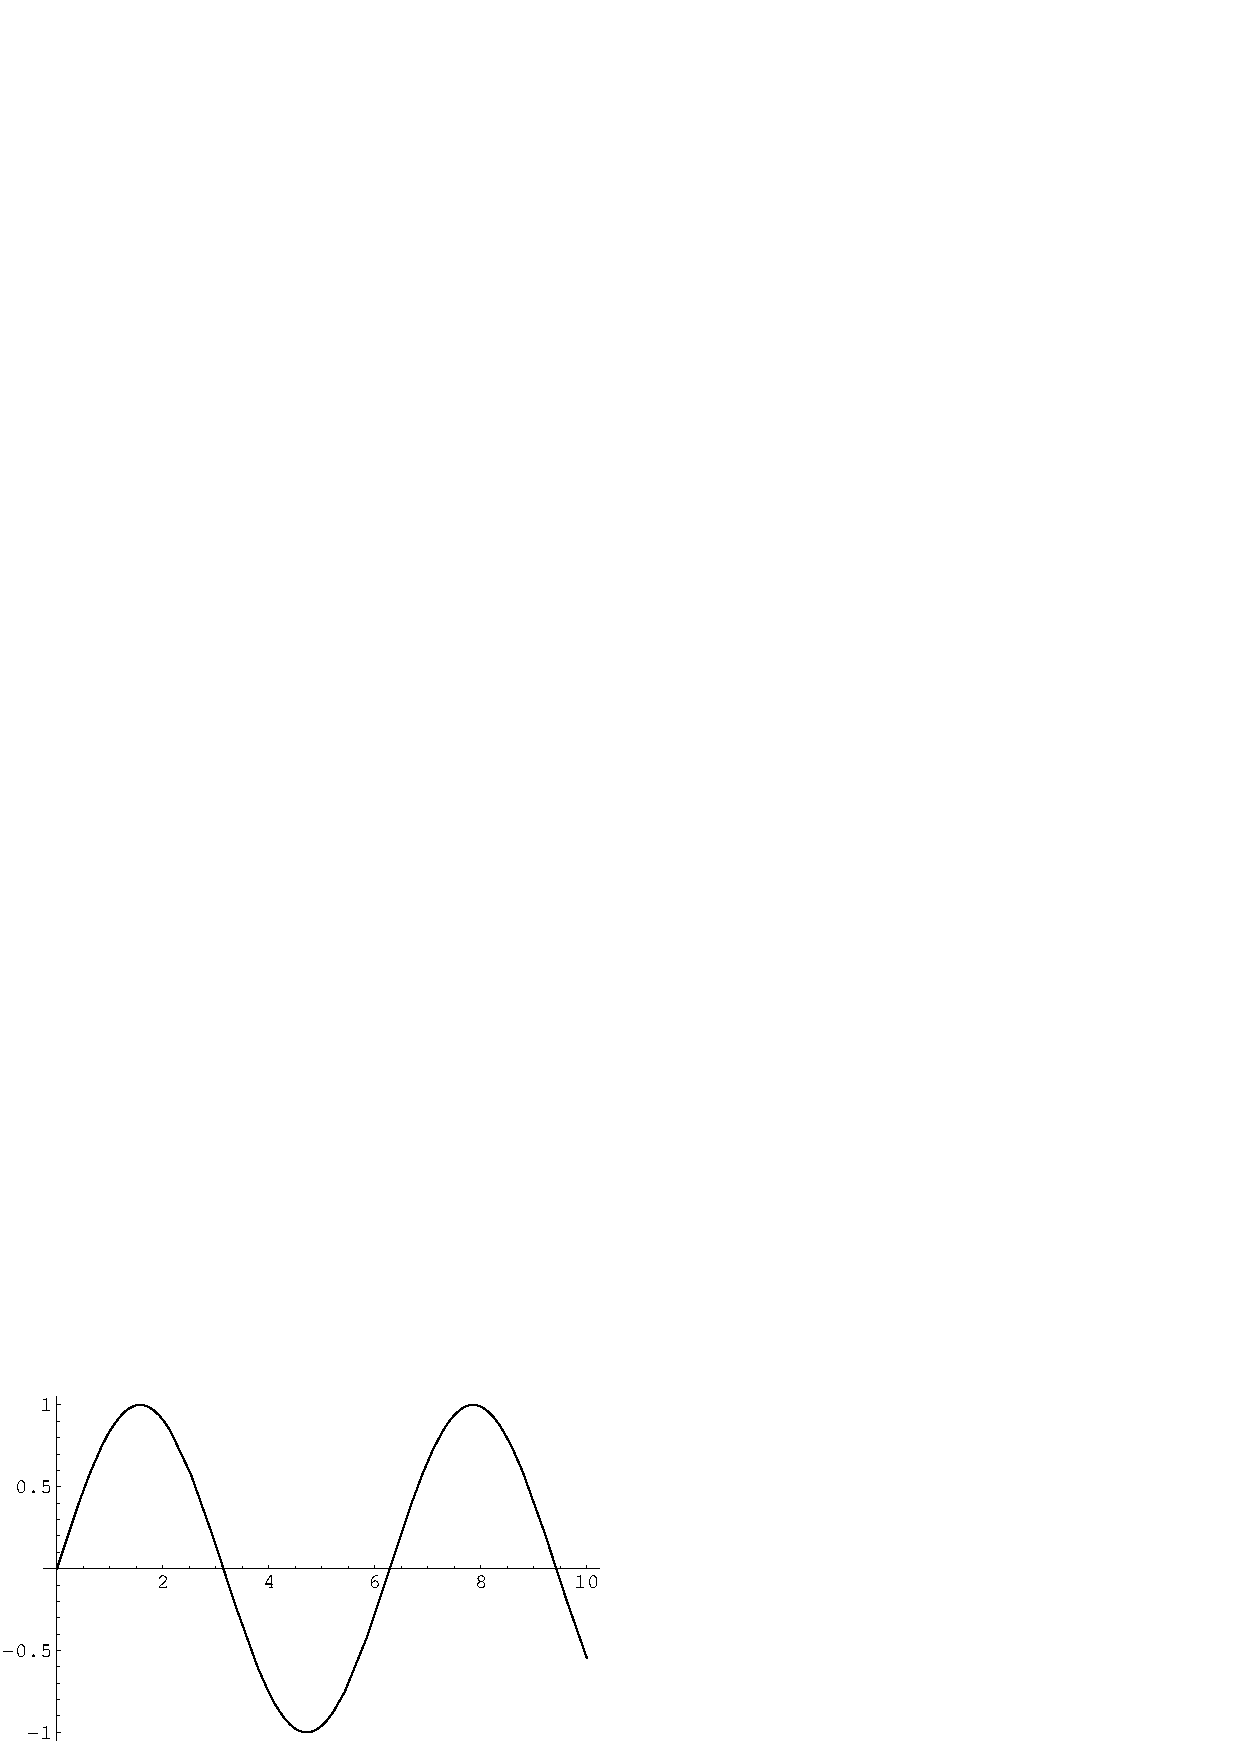
\includegraphics[width=\textwidth]{figures/mathematica}
\fcmfcaption{Ten sam wykres ale na szerokość tekstu. Formatowanie podpisu zgodne z wytycznymi FCMu.}\label{rys:plama2}
\end{figure}

Styl FCMu to nieco inne nagłówki rysunków. Dostepne są one poleceniem \texttt{fcmfcaption} (zob.~rysunek
\ref{rys:plama2}).

\subsection{Tablice}

Tablice to piękna rzecz, choć akurat ich umiejętne tworzenie w \LaTeX{}u nie jest łatwe. 
Jeśli tablica jest skomplikowana, to można ją na przykład wykonać w programie
OpenOffice, a następnie wyeksportować jako plik \akronim{PDF}. W każdym przypadku tablice wstawia się podobnie
jak rysunki, tylko że w środowisko \texttt{table}. Tradycja typograficzna sugeruje umieszczenie opisu tablicy, a więc
elementu \texttt{caption} ponad jej treścią (inaczej niż przy rysunkach).  

Tablica~\ref{tab:tabela} pokazuje pełen przykład.

\begin{table}[ht]
\caption{Przykładowa tabela. Styl opisu jest zgodny z rysunkami.}\label{tab:tabela}
\centering\footnotesize%
\begin{tabular}{l c}
\toprule
artykuł & cena [zł] \\
\midrule
bułka   & $0,4$ \\
masło   & $2,5$ \\
\bottomrule
\end{tabular}
\end{table}

Zasady FCMu sugerują nieco inne nagłówki tablic. Dostepne są one poleceniem \texttt{fcmtcaption} (zob.~tablicę
\ref{tab:tabela2}).

\begin{table}[ht]
\fcmtcaption{Przykładowa tabela. Styl opisu jest zgodny z wytycznymi FCMu.}\label{tab:tabela2}
\centering\footnotesize%
\begin{tabular}{l c}
\toprule
artykuł & cena [zł] \\
\midrule
bułka   & $0,4$ \\
masło   & $2,5$ \\
\bottomrule
\end{tabular}
\end{table}


\subsection{Checklista}

\begin{itemize}
\item Znakiem myślnika jest w LaTeXu dywiz pełen (---) albo półpauza (--), przykład:
  A niech to jasna cholera --- wrzasnąłem.

\item Połączenie między wyrazami to zwykły myślnik, przykład:   północno-zachodni

\item Sprawdź czy tutuł pracy ma maksymalnie dwa wiersze i czy stanowią one pełne frazy
  (czy nie ma przeniesienia bez sensu).

\item Sprawdź ostrzeżenia o 'overfull' i 'underful' boxes. Niektóre z nich można zignorować (spójrz
  na wynik formatowania), niektóre trzeba poprawić; czasem przeformułować zdanie.

item Przypisy stawia się wewnątrz zdań lub za kropką, przykład:
  Footnote is added after a comma.\footnote{Here is a footnote.}

\item Nie używaj przypisów zbyt często. Zobacz, czy nie lepiej będzie zintegrować przypis z tekstem.

\item Tytuły tabel, rysunków powinny kończyć się kropką.

\item Nie używaj modyfikatora [h] (here) do rysunków i tabel. Rysunki i tabele powinny być
  justowane do góry strony lub na stronie osobnej.

\item Wyróżnienie w tekście to polecenie \emph{wyraz}, nie należy używać czcionki pogrubionej (która
  wystaje wizualnie z tekstu i rozprasza).

\item Nazwy plików, katalogów, ścieżek, zmiennych środowiskowych, klas i metod formatujemy poleceniem
  \texttt{plik\_o\_pewnej\_nazwie}.

\item Po ostatniej zmianie do treści, sprawdź i przenieś wiszące spójniki wstawiając przed nie znak
  tyldy (twardej spacji), przykład:
  Ala i~kotek nie lubią mleczka, a~Stasiu lubi.
  
\item Za i.e. (id est) i e.g. (exempli gratia) stawia się zwyczajowo przecinek w typografii amerykańskiej.

\item Przed i za pełną pauza nie ma zwyczajowo spacji w typografii amerykańskiej, przykład:
  Darn, this looks good---said Mary.

\item Zamykający cudzysłów oraz footnote wychodzą za ostatni znak interpunkcji w typografii 
  amerykańskiej, przykłady:
  It can be called a ``curiosity,'' but it's actually normal.
  Footnote is added after a comma.\footnote{Here is a footnote.}

\item Odwołania do tabel i rysunków zawsze z wielkiej litery, przykład:
  In Figure~\ref{rys:plama} we illustrated XXX and in Table~\ref{tab:tabela} we show detailed data.
  
\end{itemize}


\section{Literatura i materiały dodatkowe}

Materiałów jest mnóstwo. Oto parę z nich:
\begin{itemize}
    \item \emph{The Not So Short Introduction\ldots}, która posiada również tłumaczenie 
    w języku polskim.\\
    \url{http://www.ctan.org/tex-archive/info/lshort/english/lshort.pdf}

    \item Klasy stylu \texttt{memoir} posiadają bardzo wiele informacji o składzie tekstów
    anglosaskich oraz sposoby dostosowania \LaTeX{}a do własnych potrzeb.\\
    \url{http://www.ctan.org/tex-archive/macros/latex/contrib/memoir/memman.pdf}
    
    \item Nasza grupa dyskusyjna i repozytorium Git są również dobrym miejscem aby zapytać
    (lub sprawdzić czy pytanie nie zostało już zadane).\\
    \url{https://github.com/politechnika/put-latex}

    \item Dla łaknących więcej wiedzy o systemie LaTeX podstawowym źródłem informacji
    jest książka Lamporta~\cite{Lamport1985}. Prawdziwy \emph{hardcore} to oczywiście
    \emph{The \TeX{}book} profesora Knutha~\cite{Knuth1986}.
\end{itemize}



%--------------------------------------
% Informacja o prawach autorskich
%--------------------------------------

\ppcolophon

\end{document}
